%%%%%% Compiler is <<<< Xelatex >>>>
%%%%%% Abstract in Khmer Lang. please use សេចក្តីសង្ខេប.docx, then convert to PDF and replace it with the សេចក្តីសង្ខេប page of the PDF thesis file.
%%%%% Institute of Technology of Cambodia (ITC)
%%%%% Department of Industrial Engineering / Mechanical Engineering
%%%%% Academic Year: 2025 -- 2026
%%%%% Thesis: Design and Implementation of a Vision-Based Delta Robot Pick and Place System Using ROS 2

\documentclass[12pt,a4paper]{article}

% -------------------------------------------------------
% ENCODING & FONT  (pdfLaTeX only -- not used by XeLaTeX)
% -------------------------------------------------------
% inputenc and fontenc are NOT needed with XeLaTeX (fontspec handles encoding)
% They are intentionally omitted here.

% -------------------------------------------------------
% PAGE GEOMETRY
% -------------------------------------------------------
\usepackage[top=2.54cm,bottom=2.54cm,left=2.54cm,right=2.54cm]{geometry}

% -------------------------------------------------------
% GENERAL PACKAGES
% -------------------------------------------------------
\usepackage{tabularx}
\renewcommand{\baselinestretch}{1}
\usepackage[section]{placeins}
\usepackage[nottoc,notlof,notlot]{tocbibind}
\usepackage{array}
\newcommand\ChangeRT[1]{\noalign{\hrule height #1}}
\usepackage{times}
\usepackage{enumitem}
\usepackage{indentfirst}
\usepackage{tcolorbox}
\usepackage{comment}
\usepackage{url,textcomp}
\setlength{\parindent}{0pt}
\setlength{\parskip}{18pt}

% -------------------------------------------------------
% SECTION / HEADING FONT SIZE (all 12pt bold)
% -------------------------------------------------------
\usepackage{titlesec}
\titleformat*{\section}{\fontsize{12pt}{10pt}\selectfont\bfseries}
\titleformat*{\subsection}{\fontsize{12pt}{10pt}\selectfont\bfseries}
\titleformat*{\subsubsection}{\fontsize{12pt}{10pt}\selectfont\bfseries}
\titleformat*{\paragraph}{\fontsize{12pt}{12pt}\selectfont\bfseries}
\titleformat*{\subparagraph}{\fontsize{12pt}{12pt}\selectfont\bfseries}

% -------------------------------------------------------
% SI UNITS
% -------------------------------------------------------
\usepackage{siunitx}
\usepackage{rotating}
\DeclareSIUnit{\rpm}{\text{rpm}}

% -------------------------------------------------------
% CODE LISTINGS  (Python / MATLAB)
% -------------------------------------------------------
\usepackage{listings}
\usepackage[framed,numbered,autolinebreaks,useliterate]{mcode} % MATLAB
% mcode.sty must be present in the same folder as main.tex

% -------------------------------------------------------
% BIBLIOGRAPHY  (APA style via biblatex + biber)
% -------------------------------------------------------
\usepackage[english]{babel}
\usepackage[
  backend=biber,
  style=apa,
]{biblatex}
\addbibresource{Main-pages/mybib.bib}

% -------------------------------------------------------
% GRAPHICS
% -------------------------------------------------------
\usepackage{graphicx}
\graphicspath{{image/}}
\usepackage[hidelinks]{hyperref}

% -------------------------------------------------------
% SPACING & MATH
% -------------------------------------------------------
\usepackage{parskip}
\setlength{\parskip}{1.5pt}
\usepackage{setspace}
\usepackage{amsmath}
\usepackage{amsfonts}
\usepackage{amsthm}
\usepackage{amssymb}
\renewcommand{\baselinestretch}{1.5}

% -------------------------------------------------------
% KHMER / XELATEX SETTINGS  (XeLaTeX ONLY -- see compiler note above)
% -------------------------------------------------------
\usepackage{iftex}
\ifXeTeX
  \XeTeXlinebreaklocale "KHM"
  \XeTeXlinebreakskip=0pt plus 2pt minus 1.5pt
\else
  \errmessage{ERROR: This thesis requires XeLaTeX. In Overleaf: Menu > Compiler > XeLaTeX}
\fi

% -------------------------------------------------------
% CUSTOM EQUATION ENVIRONMENT (centred + bold label)
% -------------------------------------------------------
\newenvironment{cequation}
  {\begin{equation*}\hspace{1.27cm}\refstepcounter{equation}}
  {\hspace{1.27cm}\textbf{(\theequation)}\end{equation*}\ignorespacesafterend}
\patchcmd{\equation}{\tagform@{\theequation}}{}{}{}
\DeclareMathOperator{\atantwo}{atan2}

% -------------------------------------------------------
% NOMENCLATURE
% -------------------------------------------------------
\usepackage[intoc]{nomencl}
\makenomenclature
\usepackage{etoolbox}
\renewcommand{\nomname}{\centering ABBREVIATIONS AND SYMBOLS}
\renewcommand{\thefigure}{\arabic{section}\arabic{figure}}
\numberwithin{table}{section}
\usepackage{xpatch}
\patchcmd{\thenomenclature}
  {\leftmargin\labelwidth}
  {\leftmargin\labelwidth\itemindent 1em}
  {}{}
\setlength{\nomlabelwidth}{3cm}

% -------------------------------------------------------
% FIGURES & TABLES CAPTIONS / NUMBERING
% -------------------------------------------------------
\usepackage{tikz}
\usepackage{tocloft}
\renewcommand\cftfigpresnum{\bfseries\figurename~}
\setlength\cftfignumwidth{7em}
\renewcommand\cfttabpresnum{\bfseries\tablename~}
\setlength\cfttabnumwidth{7em}
\usetikzlibrary{shapes.geometric, arrows}
\usepackage[labelfont=bf]{caption}
\captionsetup{labelfont=bf}
\usepackage{caption}
\captionsetup[table]{labelsep=space}
\renewcommand{\thetable}{{\thesection.\arabic{table}.}}
\captionsetup[figure]{labelsep=space}
\renewcommand{\thefigure}{\thesection.\arabic{figure}.}

% -------------------------------------------------------
% HEADER / FOOTER
% -------------------------------------------------------
\usepackage{fancyhdr}
\usepackage{lastpage}
\renewcommand{\headrulewidth}{0pt}
\fancyhead[R,LO]{}
\fancyhead[L,RO]{}

% -------------------------------------------------------
% APPENDIX
% -------------------------------------------------------
\usepackage[titletoc,title]{appendix}

% -------------------------------------------------------
% EQUATION NUMBERING  (bold, section-based)
% -------------------------------------------------------
\numberwithin{equation}{section}
\renewcommand{\theequation}{\textbf{Eq.\hspace{1mm}\thesection.\arabic{equation}.}}

% -------------------------------------------------------
% TABLE OF CONTENTS STYLE
% -------------------------------------------------------
\usepackage{secdot}
\sectiondot{section}
\sectiondot{subsection}
\sectiondot{subsubsection}
\renewcommand{\cftsecfont}{\mdseries}
\renewcommand{\cftsecpagefont}{\mdseries}
\renewcommand{\cftsecaftersnum}{.}
\renewcommand{\cftsubsecaftersnum}{.}
\renewcommand{\cftsubsubsecaftersnum}{.}
\setlength{\cftbeforesecskip}{1pt}
\renewcommand{\cftsecleader}{\cftdotfill{\cftdotsep}}
\renewcommand{\cftdotsep}{0.25}

% -------------------------------------------------------
% KHMER FONTS  (XeLaTeX only)
% -------------------------------------------------------
\usepackage{fontspec}
\newcommand{\KhOS}{\fontspec[Script=Khmer,Scale=0.8,Path=./]{KhmerOSSiemreap.ttf}\selectfont}
\newcommand{\KhOSsy}{\fontspec[Script=Khmer,Scale=0.92,Path=./]{KhmerOSSiemreap.ttf}\selectfont}
\newcommand{\KhOSml}{\fontspec[Script=Khmer,Scale=1,Path=./]{KhmerOSMuolLight.ttf}\selectfont}
\newfontscript{Khmer}{khmr}
\usepackage{xunicode}
\setmainfont{TeX Gyre Termes}

% -------------------------------------------------------
% DOCUMENT BEGINS
% -------------------------------------------------------
\begin{document}

  \pagenumbering{roman}

  % --- Front Matter ---
  \section*{\centering ACKNOWLEDGEMENTS}\addcontentsline{toc}{section}{ACKNOWLEDGEMENTS}
\hspace{1.27cm}
First and foremost, I would like to express my deepest gratitude to my thesis advisor, \textbf{Asst.\ Prof.\ Dr.\ SRANG Sarot}, Head of ECAM-LaSalle Phnom Penh and the Dynamics and Control Laboratory, and \textbf{Mr.\ SREY Sokserey}, for their invaluable guidance, continuous support, and encouragement throughout the course of this research. Their expertise and dedication to providing constructive feedback, despite their demanding schedules, have been instrumental in shaping this work and guiding it to completion.

\par
\hspace{1.27cm}
I would also like to extend my sincere appreciation to \textbf{H.E.\ Prof.\ Dr.\ PO Kimtho}, the Director of the Institute of Technology of Cambodia, and \textbf{Dr.\ CHAN Sarin}, the Head of the Department of Industrial Engineering and Mechanical Engineering, for their exceptional leadership and for providing an excellent academic environment and the necessary resources to carry out this research.
\par
\hspace{1.27cm}
My heartfelt thanks go to all the faculty members and staff of the Department of Industrial Engineering and Mechanical Engineering at the Institute of Technology of Cambodia for their academic support and inspiration throughout my studies.
\par
\hspace{1.27cm}
I am also deeply grateful to my colleagues at ECAM-LaSalle Phnom Penh and the Dynamics and Control Laboratory (DCLab) for their constant assistance and guidance, particularly during the hands-on phases of this project involving fabrication, machining, and system integration. Their willingness to share knowledge and help overcome technical obstacles proved vital to the success of this work.
\par
\hspace{1.27cm}
I am deeply grateful to my family for their unconditional love, sacrifice, and encouragement. Their unwavering belief in me has been my greatest source of motivation from the beginning to the end of my studies. Their support and generosity have made this journey possible.
\par
\hspace{1.27cm}
Finally, I wish to thank my friends and colleagues for their assistance, discussions, and moral support during the development of this project.
  \section*{\centering \KhOSml សេចក្តីសង្ខេប}
\vspace{2.5mm}
\addcontentsline{toc}{section}{\KhOSml សេចក្តីសង្ខេប}
{\KhOS
\hspace{1.27cm}
    % TODO: Write your Khmer abstract here.
    % Recommended: Use a Khmer word processor (e.g., LibreOffice with Khmer OS fonts)
    % to draft the text, then paste it here.
    %
    % The abstract should cover:
    % - Background and motivation of the Delta Robot research
    % - Methods used (mechanical design, kinematics, control)
    % - Key results and findings
    % - Contribution to robotics in Cambodia
    %
    % Example placeholder (replace with your actual Khmer text):
និក្ខេបបទនេះបង្ហាញពីការរចនា ការអភិវឌ្ឍ និងការផ្ទៀងផ្ទាត់ពិសោធន៍នៃប្រព័ន្ធ Delta robot លើកដាក់វត្ថុដែលប្រើប្រព័ន្ធចក្ខុវិស័យ ដោយប្រើ ROS 2 ក្នុងគោលបំណងផ្តល់នូវដំណោះស្រាយរ៉ូបូទិចដែលមានតម្លៃសមរម្យ និងមានប្រសិទ្ធភាព សម្រាប់ការអប់រំ និងការប្រើប្រាស់ឧស្សាហកម្មនៅប្រទេសកំពុងអភិវឌ្ឍន៍ ដោយផ្តោតជាពិសេសទៅលើប្រទេសកម្ពុជា។ Delta robot ដែលល្បីល្បាញដោយសាររចនាសម្ព័ន្ធចលនាស្របតទួល (parallel kinematic) និងសមត្ថភាពលើកដាក់វត្ថុដោយល្បឿនខ្ពស់ ត្រូវបានអនុវត្តជាប្រព័ន្ធស្វយ័តពេញលេញ ដែលបូករួមចក្ខុវិស័យកុំព្យូទ័រ ការគ្រោងផែនការចលនាក្នុងពេលវេលាជាក់ស្តែង និងការដំណើរការតាមបណ្តាញ CAN bus។
    \par
    \hspace{1.27cm}
    % [Add more Khmer paragraphs here]
    រ៉ូបូនេះត្រូវបានសាងសង់ដោយប្រើប្រដាប់ដំណើរការ RobStride RS-00 quasi-direct-drive ចំនួនបី ដែលត្រូវបានគ្រប់គ្រងតាម CAN bus ដំណើរការ ១ Mbit/s ស៊ុមរចនាសម្ព័ន្ធផ្លាស់ប្ដូររ (aluminum) និងបោះពុម្ព 3D ដោយមានប៉ារ៉ាម៉ែត្រធ្យូមគ្នា f = 157 mm, e = 35 mm, rf = 200 mm និង re = 400 mm ព្រមទាំង gripper ដ្រេសខ្យល់ (pneumatic solenoid gripper)។ ក្របខ័ណ្ឌកម្មវិធីប្រភពបើកចំហ រួមមាន Robot Operating System 2 (ROS 2) និង Python ត្រូវបានប្រើសម្រាប់ការគ្រោងផែនការចលនា ការគណនា kinematics និងការគ្រប់គ្រងពេលវេលាជាក់ស្តែង។ ប្រព័ន្ធចក្ខុវិស័យប្រើប្រាស់កាមេរ៉ា Intel RealSense D455 stereo depth ដែលផ្តល់ស្ទ្រីម RGB និង depth តម្រឹម (aligned) ដល់ ៣០ fps រួមជាមួយការរកឃើញវត្ថុក្នុងទំហំពណ៌ HSV (ដែលអាចប្ដូរជំនួស YOLO11n backbone បាន) សម្រាប់ការកំណត់ទីតាំងវត្ថុក្នុងពេលជាក់ស្តែង។ កូអរដោនេ pixel ដែលបានរកឃើញ ត្រូវបានព្យាករបញ្ច្រាសទៅជាកូអរដោនេ 3D ក្នុងស៊ុមកាមេរ៉ា ដោយប្រើម៉ូដែល pinhole ហើយបំប្លែងទៅស៊ុមមូលដ្ឋានរ៉ូបូតាមរយៈការបំប្លែង rigid-body ដែលបានកែតម្រូវ (calibrated)។
    \par
    \hspace{1.27cm}
    % [Add more Khmer paragraphs here]
    រ៉ូបូដែលបានអភិវឌ្ឍមានសេរីភាពចំណាកក្នុង ៣ ទិសដែលប្រតិបត្តិការក្រោម preset ចលនាមធ្យម ដោយ end-effector មានល្បឿនអតិបរមា vmax = 2000 mm/s និងសំទុះ amax = 5000 mm/s²។ គំរូ kinematic រួមមាន forward និង inverse kinematics ត្រូវបានទាញចេញតាមរបៀប analytic ដោយអនុវត្តតាមរូបមន្ត Trossen Robotics ហើយបានផ្ទៀងផ្ទាត់តាមការសាកល្បងរូបវ័ន្ត ដោយសម្រេចបាននូវកំហុស FK position ទាបជា ០,៥ mm ជាប់លាប់។ ការកែតម្រូវវ loop feedforward ដោយប្រើចក្ខុវិស័យ end-effector តាមដាន EE laser marker ក្នុងស៊ុមកាមេរ៉ា ហើយកែតម្រូវទីតាំងចូលទៅដំណើរការ (approach position) បន្តបន្ទាប់មុនពេលចុះ ដើម្បីបង្កើនភាពត្រឹមត្រូវក្នុងការលើករបស់នៅក្នុងទំហំការងារដែលមិនស្មើ (non-linear workspace)។ ការព្យាករខ្សែក្រវ៉ាត់ (conveyor belt prediction) ត្រូវបានអនុវត្តដោយប្រើទម្រង់ចលនាត្រីកោណ (triangular motion profile) ដើម្បីទូទាត់ចំពោះពេលវេលាធ្វើដំណើររ៉ូបូ នៅពេលលើកវត្ថុដែលកំពុងផ្លាស់ទី ក្នុងល្បឿនខ្សែក្រវ៉ាត់ ១២,៨៥ mm/s ។
    \par
    \hspace{1.27cm}
    សរុបមក ការស្រាវជ្រាវនេះបង្ហាញពីបំពង់ (pipeline) ពេញលេញពី vision ទៅ motion សម្រាប់ការលើកដាក់វត្ថុដោយស្វ័យ័ត ផ្អល់ platform Delta robot ដែលអាចចម្លងបាន (replicable) ដែលមានការចំណាយទាប និងលើកទឹកចិត្តការកសាងសមត្ថភាពក្នុងស្រុក ក្នុងវិស័យ robotics និង automation engineering នៅប្រទេសកម្ពុជា។
    % [Add concluding Khmer paragraph here]
}
        % Khmer Abstract
  \section*{\centering ABSTRACT}\addcontentsline{toc}{section}{ABSTRACT}
\hspace{1.27cm}
This thesis presents the design, development, and experimental validation of a vision-based Delta robot pick-and-place system using ROS 2, aimed at providing an affordable and functional robotic solution for educational and industrial applications in developing countries, with a particular focus on Cambodia. The Delta robot, known for its parallel kinematic structure and high-speed pick-and-place capability, is implemented as a complete autonomous system integrating computer vision, real-time motion planning, and CAN bus actuation.

\par
\hspace{1.27cm}
The robot is constructed using three RobStride RS-00 quasi-direct-drive actuators controlled via CAN bus at 1\,Mbit/s, an aluminum and 3D-printed structural frame with geometric parameters $f=157$\,mm, $e=35$\,mm, $r_f=200$\,mm, and $r_e=400$\,mm, and a pneumatic solenoid gripper. Open-source software frameworks including Robot Operating System 2 (ROS\,2) and Python are employed for motion planning, kinematics computation, and real-time control. The vision system uses an Intel RealSense D455 stereo depth camera providing aligned RGB and depth streams at up to 30\,fps, combined with a HSV colour-space object detection (with YOLO11n 
interchangeable backbone) for real-time object localisation. Detected pixel coordinates are back-projected to 3D camera-frame coordinates using the pinhole model and transformed to the robot base frame via a calibrated rigid-body transform.

\par
\hspace{1.27cm}
The developed robot features three translational degrees of freedom and operates under a medium motion preset with end-effector velocity $v_{\max}=2000$\,mm/s and acceleration $a_{\max}=5000$\,mm/s$^2$. The kinematic model, including forward and inverse kinematics, was derived analytically following the Trossen Robotics formulation and validated through physical testing, achieving FK position errors consistently below 0.5\,mm. A visual end-effector feedforward correction loop tracks the EE laser marker in the camera frame and iteratively corrects the approach position prior to descent, improving pick accuracy across the non-linear workspace. Conveyor belt prediction is implemented using a triangular motion profile to compensate for robot travel time when picking moving objects at a measured belt speed of 12.85\,mm/s.

\par
\hspace{1.27cm}
Overall, this research demonstrates a complete vision-to-motion pipeline for autonomous pick-and-place, contributes a replicable low-cost Delta robot platform, and promotes local capacity building in robotics and automation engineering in Cambodia.

  \printnomenclature
%% This will add the subgroups
%----------------------------------------------
\renewcommand\nomgroup[1]{%
  \item[\bfseries
  \ifstrequal{#1}{A}{%
  \ifstrequal{#1}{B}{%
}}%
]}
%----------------------------------------------
\mbox{}

%___________ ABBREVIATIONS ________________
\nomenclature[A]{\textbf{DOF}}{Degree of Freedom.}
\nomenclature[A]{\textbf{DC}}{Direct Current.}
\nomenclature[A]{\textbf{ROS\,2}}{Robot Operating System 2.}
\nomenclature[A]{\textbf{PC}}{Personal Computer.}
\nomenclature[A]{\textbf{CAD}}{Computer Aided Design.}
\nomenclature[A]{\textbf{2D}}{Two Dimensional.}
\nomenclature[A]{\textbf{3D}}{Three Dimensional.}
\nomenclature[A]{\textbf{FK}}{Forward Kinematics.}
\nomenclature[A]{\textbf{IK}}{Inverse Kinematics.}
\nomenclature[A]{\textbf{BLDC}}{Brushless DC Motor.}
\nomenclature[A]{\textbf{FOC}}{Field Oriented Control.}
\nomenclature[A]{\textbf{CAN}}{Controller Area Network.}
\nomenclature[A]{\textbf{RPM}}{Revolutions per Minute.}
\nomenclature[A]{\textbf{EE}}{End-Effector.}
\nomenclature[A]{\textbf{FSM}}{Finite State Machine.}
\nomenclature[A]{\textbf{YOLO}}{You Only Look Once (object detection algorithm).}
\nomenclature[A]{\textbf{RGB-D}}{Red-Green-Blue and Depth image.}
\nomenclature[A]{\textbf{HSV}}{Hue-Saturation-Value colour space.}
\nomenclature[A]{\textbf{FPS}}{Frames Per Second.}
\nomenclature[A]{\textbf{QDD}}{Quasi-Direct-Drive actuator.}
\nomenclature[A]{\textbf{PP mode}}{Position-Profile control mode.}

%%____________ SYMBOLS ____________
\nomenclature[B]{$v$}{Velocity (\(m/s\)).}
\nomenclature[B]{$\omega$}{Angular Velocity (\(rad/s\)).}
\nomenclature[B]{$T$}{Torque (\(N \cdot m\)).}
\nomenclature[B]{$F$}{Force (\(N\)).}
\nomenclature[B]{$r$}{Radius (\(m\)).}
\nomenclature[B]{$r_f$}{Length of Upper Arm Link (\(m\)).}
\nomenclature[B]{$r_e$}{Length of Lower Arm Link (\(m\)).}
\nomenclature[B]{$e$}{Side Length of Moving Platform Triangle (\(m\)).}
\nomenclature[B]{$f$}{Side Length of Fixed Base Triangle (\(m\)).}
\nomenclature[B]{$\theta_i$}{Joint Angle of $i$-th Arm (\(rad\)).}
\nomenclature[B]{$(x,y,z)$}{Cartesian Position of End-Effector (\(mm\)).}
\nomenclature[B]{$(u,v)$}{Pixel Coordinates in Image Frame (\(px\)).}
\nomenclature[B]{$f_x, f_y$}{Camera Focal Lengths in $x$ and $y$ (\(px\)).}
\nomenclature[B]{$c_x, c_y$}{Camera Principal Point Coordinates (\(px\)).}
\nomenclature[B]{$Z$}{Depth from Camera to Object (\(mm\)).}
\nomenclature[B]{$\mathbf{R}$}{Rotation Matrix of Camera-to-Robot Transform.}
\nomenclature[B]{$\mathbf{t}$}{Translation Vector of Camera-to-Robot Transform (\(mm\)).}
\nomenclature[B]{$v_y$}{Conveyor Belt Velocity in $Y$ direction (\(mm/s\)).}
\nomenclature[B]{$t_{\text{total}}$}{Total Prediction Delay (\(s\)).}
\nomenclature[B]{$a_{\max}$}{Maximum End-Effector Acceleration (\(mm/s^2\)).}
\nomenclature[B]{$v_{\max}$}{Maximum End-Effector Velocity (\(mm/s\)).}
\nomenclature[B]{$K$}{EE Correction Proportional Gain (dimensionless).}
\nomenclature[B]{$J$}{Jacobian Matrix.}
\nomenclature[B]{$g$}{Gravitational Acceleration (\(m/s^2\)).}


  % --- Tables of Contents / Figures / Tables ---
  \begin{center}
    \renewcommand{\contentsname}{\centering \normalsize TABLE OF CONTENTS}
    \addcontentsline{toc}{section}{\contentsname}
    \tableofcontents
    \clearpage
    \renewcommand{\listfigurename}{\normalsize LIST OF FIGURES}
    \addcontentsline{toc}{section}{\listfigurename}
    \listoffigures
    \clearpage
    \renewcommand{\listtablename}{\normalsize LIST OF TABLES}
    \addcontentsline{toc}{section}{\listtablename}
    \listoftables
    \clearpage
  \end{center}

  \setcounter{enumi}{3}
  \cleardoublepage
  \pagenumbering{arabic}
  \pagestyle{fancy}
  \cfoot{\thepage}

  % --- Main Chapters ---
  \section{INTRODUCTION}

%============================================================================
\subsection{Background}
\hspace{1.27cm}
The manufacturing and automation sectors have been evolving rapidly in recent years, with
robotic systems taking on a central role in improving speed, accuracy, and consistency
across many industries. One robotic design that has proven particularly effective in this
context is the Delta robot, a parallel kinematic manipulator first developed by Professor
Reymond Clavel at the \'{E}cole Polytechnique F\'{e}d\'{e}rale de Lausanne (EPFL) in 1985.
Since its introduction, the Delta robot has been widely deployed in demanding industrial
environments including food processing, pharmaceutical production, and electronics
manufacturing, where speed and precision are critical \autocite{clavel-1990}.
\par
\hspace{1.27cm}
What sets the Delta robot apart from conventional serial link manipulators is its parallel
kinematic structure, where all actuators remain mounted on a fixed base rather than along
the moving links. This keeps the end effector platform extremely lightweight, reduces
inertia, and allows the robot to achieve cycle times and repeatability levels that serial
arms simply cannot match. The mechanical design typically involves three identical kinematic
chains, each made up of a motor driven upper arm and a passive lower parallelogram linkage,
working together to position the moving platform precisely within the robot's workspace
\autocite{merlet-2006}.
\par
\hspace{1.27cm}
In parallel with these mechanical developments, the field of robot perception has advanced
considerably. The availability of affordable RGB-D cameras such as the Intel RealSense
series, combined with powerful deep learning based object detectors like YOLO, has made
real time 3D object localisation practical even outside of well funded research labs. When
paired with open source middleware like Robot Operating System 2 (ROS\,2), these tools make
it possible to build complete perception to motion pipelines that would previously have
required expensive proprietary systems.
\par
\hspace{1.27cm}
Despite these technological advances, the practical adoption of Delta robots and automated
systems more broadly remains limited in developing countries like Cambodia. High import
costs, inconsistent access to specialised hardware, and a limited local pool of engineers
trained in advanced robotics all contribute to this gap. Small manufacturers and
educational institutions in particular often lack the resources and technical support needed
to bring robotic automation into their operations.
\par
\hspace{1.27cm}
For Cambodia specifically, this gap represents a missed opportunity at a critical moment
in the country's industrial development. The food and agricultural processing sector,
which handles large volumes of rice, cassava, and packaged goods for export, still depends
heavily on manual labour for sorting and packaging tasks that Delta robots are ideally
suited to handle. Meanwhile, the Special Economic Zones around Phnom Penh and Sihanoukville
are attracting increasing foreign investment in light electronics and component assembly,
where pick and place precision and throughput directly affect competitiveness. An affordable
vision guided Delta robot system built on open source tools could offer local factories a
genuine path toward automation without the burden of expensive vendor contracts or imported
technical expertise. Beyond the factory floor, such a system also creates a concrete
platform for robotics education, helping Cambodian universities and technical institutes
train the next generation of engineers in skills such as computer vision, real time control,
and kinematics that are currently difficult to develop locally.
\par
\hspace{1.27cm}
This thesis responds to these needs by presenting the design, development, and experimental
validation of a vision based Delta robot pick and place system built on ROS\,2 using
affordable and accessible components. The system brings together a RealSense D455 depth
camera, YOLO based object detection, CAN bus motor control for three RobStride 00
actuators, and a visual end effector feedforward correction loop, all integrated within a
modular ROS\,2 architecture. The goal is to demonstrate that a fully functional vision to
motion pipeline is achievable at low cost, and to offer a replicable foundation for robotic
automation and engineering education in Cambodia and similar emerging economies.
%============================================================================
\subsection{Statement of Problem}
\hspace{1.27cm}
Commercial Delta robots offer excellent speed and accuracy but are prohibitively expensive for educational institutions and small-scale manufacturers in developing countries. Import costs, limited local technical expertise, and the absence of affordable open-source implementations create significant barriers to adoption. At the same time, the integration of computer vision into robot control introduces additional engineering challenges: coordinate frame calibration between the camera and robot, accurate 2D localization from YOLO object detection, compensation for non-linear kinematic errors across the workspace, and real-time synchronization between detection and motion planning.

\par
\hspace{1.27cm}
Existing low-cost Delta robot implementations typically rely on 2D monocular cameras with fixed-height assumptions, limiting their ability to handle objects at arbitrary heights or on moving conveyors. Furthermore, most implementations do not include closed-loop visual feedback to compensate for mechanical and calibration errors, resulting in systematic pick misses that degrade pick success rates.

\par
\hspace{1.27cm}
This thesis addresses these problems by designing a complete vision to motion pipeline that uses color detecting for 2D object detection, a calibrated rigid-body transform for camera to robot coordinate, conveyor belt for moving object picking, and a visual end-effector feedforward correction loop that iteratively minimizes the pixel-space error between the detected object and the EE marker before descent.

%============================================================================
\subsection{Goal and Objective}
\subsubsection{Goal}
\hspace{1.27cm}
The goal of this thesis is to design, develop, and validate a vision based Delta robot system capable of autonomously performing pick and place tasks on conveyor belt, using a RealSense D455 depth camera, YOLO object detection, and ROS\,2 for real-time control.

\subsubsection{Objective}
\hspace{1.27cm}
To achieve this goal, the following objectives are established:
\begin{itemize}
    \item Design and develop a functional prototype of the Delta Robot Parallel Manipulator.
    \item To visualize, generate and control trajectory for pick and place
\end{itemize}

%============================================================================
\subsection{Scope and Limitation}
\subsubsection{Scope}
\hspace{1.27cm}
The scope of this thesis includes:
\begin{itemize}
    \item Mechanical design and fabrication of the Delta robot structure using aluminum profiles and 3D-printed parts.
    \item Selection and integration of three RobStride RS-00 actuators via CAN bus at 1\,Mbit/s for each kinematic chain.
    \item Implementation of a ROS\,2 control architecture
    \item Integration of an Intel RealSense D455 depth camera for RGB object detection
    \item Implementation of a YOLO-based object detection node and full camera-to-robot coordinate transform pipeline.
    \item Visual end effector tracking using a laser dot marker and correction loop.
    \item Integration of a pneumatic solenoid gripper.
    \item Testing and demonstration of pick and place operations within the defined workspace.
\end{itemize}

\subsubsection{Limitation}
\hspace{1.27cm}
The limitations of this thesis are:
\begin{itemize}
    \item Single object class: The YOLO detector is trained for a single object class (orange blob); multi-class sorting is not implemented.
    \item No gripper feedback: The pneumatic gripper has no force or contact sensing; pick success is unverified (open-loop grasp).
    \item No GUI 
\end{itemize}

  %============================================================================
% CHAPTER 2: LITERATURE REVIEW
% Institute of Technology of Cambodia
% Delta Robot Vision-Based Control System
% Academic Year: 2025-2026
%============================================================================

\section{LITERATURE REVIEW}

\subsection{State-of-the-Art}
\hspace{1.27cm}
This chapter examines the body of knowledge underpinning the design and
implementation of the proposed system. Topics covered include the
historical development and kinematic theory of Delta robots, techniques
for vision-based localisation of objects in a robot workspace, deep
learning approaches to object detection, the mathematical basis for
transforming coordinates between camera and robot frames, and
software frameworks for real-time motion control. Several published
implementations of low-cost, vision-guided Delta robot systems are
also reviewed and compared to contextualise the contributions made in
this work.

%============================================================================
\subsubsection{History and Concept of Delta Robotics}
\hspace{1.27cm}
The Delta robot emerged from research conducted by Professor Reymond
Clavel at the \'{E}cole Polytechnique F\'{e}d\'{e}rale de Lausanne
(EPFL) in 1985, motivated by the need for a manipulator capable of
handling lightweight objects at speeds that conventional serial robots
could not achieve \autocite{clavel-1990}, as shown in
\textbf{\autoref{fig:first_delta_robot}}. The mechanism is built
around a parallel kinematic structure in which three mechanically
identical limbs connect a stationary base to a moving end-effector
platform. Each limb consists of a proximal arm driven directly by a
rotary actuator mounted on the base, and a distal forearm formed by a
passive parallelogram linkage. The geometric effect of these
parallelogram linkages is to restrict the platform to purely
translational movement, meaning the orientation of the end-effector
remains fixed regardless of where within the workspace it is
positioned. This constraint yields exactly three translational degrees
of freedom (DOF).

\begin{figure}[h]
    \centering
    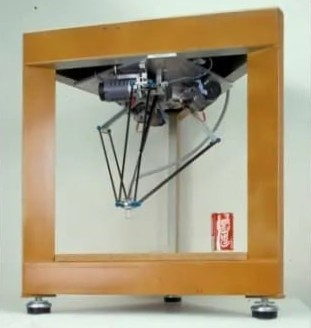
\includegraphics[width=0.55\linewidth]{image/first_delta_robot.jpg}
    \caption{The First Delta Robot Prototype Developed by Professor
             Reymond Clavel at the \'{E}cole Polytechnique
             F\'{e}d\'{e}rale de Lausanne (EPFL) in 1985
             \autocite{clavel-1990}.}
    \label{fig:first_delta_robot}
\end{figure}

\par
\hspace{1.27cm}
Because all three actuators are fixed to the stationary base, the
only mass in motion during operation is the lightweight platform
itself, which dramatically reduces the effective inertia of the system
and allows the mechanism to complete a full pick-and-place cycle in
under one second. Clavel formally documented the kinematic
architecture in U.S.\ Patent 4,976,582, and subsequent analyses by
researchers in the robotics community have validated and extended
the original kinematic formulations \autocite{merlet-2006,
stock-2003}. Industrially, this architecture has proven highly
successful: commercial variants produced by ABB (marketed as the
FlexPicker) and by Fanuc routinely achieve positional repeatability
figures of $\pm$0.1\,mm alongside cycle times shorter than
0.3\,seconds, establishing the Delta robot as the leading platform
for high-volume pick-and-place in food processing, pharmaceutical
packaging, and electronics manufacturing \autocite{pierrot-1991}.

%============================================================================
\subsubsection{Recent Research and Applications}
\hspace{1.27cm}
The three case studies reviewed below were chosen on the basis that
each shares key technical elements with the system developed in this
thesis, namely a vision-guided Delta robot, real-time object
detection, and a design approach oriented toward low manufacturing
cost.

\begin{itemize}
    \item \textbf{Case Study 1: Visual Servo Kinematic Control of
    Delta Robot Using YOLOv5 Algorithm.}\par
    \hspace{1.27cm}
    Among the works reviewed, this study bears the closest structural
    resemblance to the system proposed here. It establishes a
    continuous vision-to-motion pipeline that begins with YOLO-based
    object detection, proceeds through a hand-eye coordinate mapping
    stage, and terminates in analytical IK computation and motor
    activation, as illustrated in \textbf{\autoref{fig:case1_image}}.
    \autocite{yamtuan-2023} constructed their robot with proximal and
    distal arm lengths of 200\,mm and 500\,mm respectively, and
    selected three Yaskawa AC servo motors driven via an Arduino Due
    board as the actuation system. Under test conditions the platform
    achieved a maximum tracking velocity of 214.55\,mm/s and a
    worst-case positioning error of 1.36\,mm. Object positions were
    estimated purely in the horizontal plane from RGB image
    coordinates, treating the vertical pick height as a constant
    known value. A notable weakness of this implementation is that
    motor commands are issued through low-level PWM signals generated
    directly from the microcontroller, with no modular software layer
    separating the perception and motion subsystems.\par
    \hspace{1.27cm}
    The perception subsystem relied on a standard 30\,fps USB webcam
    capturing frames at $640 \times 480$\,pixels, with the YOLOv5
    detector integrated into a Python and OpenCV processing pipeline.
    Hand-eye calibration was performed by rotating the camera
    coordinate frame by $\beta = 150^{\circ}$ relative to the robot
    base frame and establishing a scale factor of 0.834\,mm/pixel
    through a linear regression procedure. During evaluation, the
    system successfully sorted eight medicine boxes of four different
    classes within 46\,seconds. Detection quality was assessed at a
    training mean average precision of 85\% and a validation score
    of 81\%, with spatial localisation errors remaining below
    3.5\,mm for unoccluded objects \autocite{yamtuan-2023}.\par
    \begin{figure}[h]
        \centering
        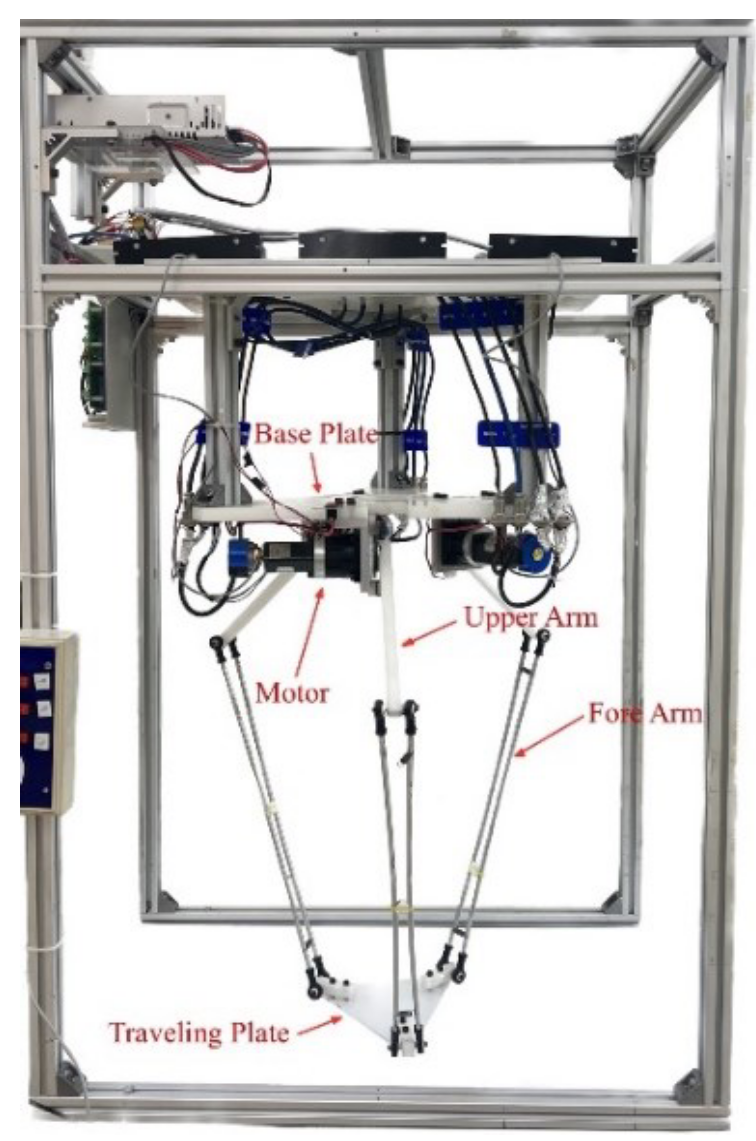
\includegraphics[width=0.4\linewidth]{image/Study Case 1.png}
        \caption{Delta robot platform employing YOLOv5-based visual
                 servoing for automated sorting of medicine boxes
                 \autocite{yamtuan-2023}.}
        \label{fig:case1_image}
    \end{figure}

    \item \textbf{Case Study 2: Design a Low-Cost Delta Robot Arm for
    Pick-and-Place Applications Based on Computer Vision.}\par
    \hspace{1.27cm}
    This work investigated the extent to which vision-based
    pick-and-place can be realised on a Delta robot built entirely
    from inexpensive, off-the-shelf parts \autocite{le-2023}. To
    minimise fabrication expense, the structural frame shown in
    \textbf{\autoref{fig:case2_image}} was produced through a
    combination of laser cutting and fused deposition modelling, a
    strategy that preserved adequate mechanical rigidity for
    bench-scale operation while avoiding the cost of machined
    components. Stepper motors replaced the servo actuators typical
    of higher-cost designs, and an Arduino Uno board was used as the
    central controller, accepting target coordinates and issuing the
    corresponding step sequences to each joint.\par
    \hspace{1.27cm}
    Object positions in the workspace were derived from images
    captured by a single fixed-overhead camera, eliminating the
    requirement for depth sensing hardware. Under the assumption that
    all target objects rest on a flat surface at a uniform, pre-measured
    height, the horizontal spatial coordinates could be back-calculated
    from the detected pixel location using the known camera geometry
    and pre-calibrated intrinsic parameters. An additional capability
    of this system was the estimation of object width from bounding
    box dimensions, which was used to set the gripper jaw separation
    dynamically before each grasp, enabling the robot to accommodate
    objects of different sizes within the same operational cycle.\par
    \hspace{1.27cm}
    Validation trials were carried out on three target objects
    differing in both geometry and dimensions. Across these trials the
    system demonstrated consistent detection, correct spatial
    estimation, and successful grasp-and-place sequences, supporting
    the conclusion that centimetre-level accuracy is attainable with
    monocular vision and low-cost mechanical hardware \autocite{le-2023}.\par
    \begin{figure}[h]
        \centering
        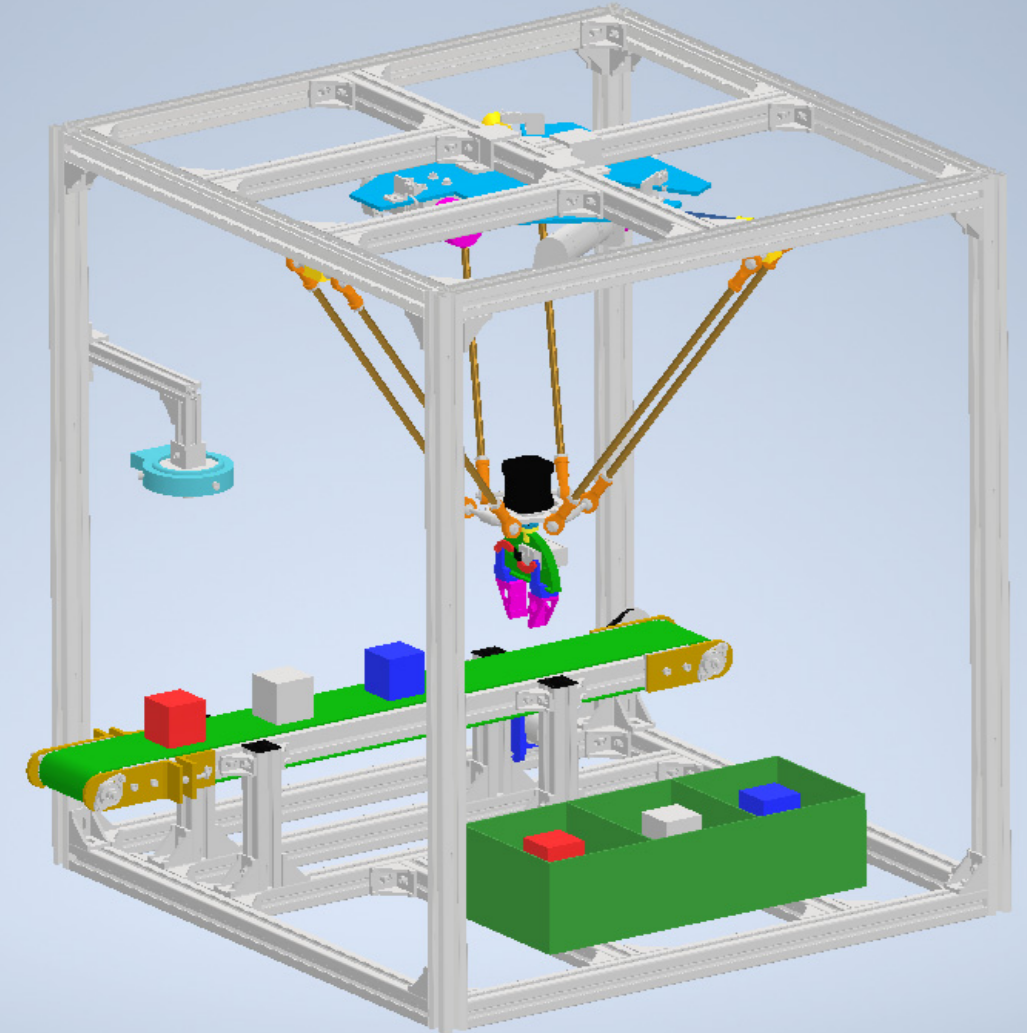
\includegraphics[width=0.5\linewidth]{image/Autodesk Study Case2.png}
        \caption{Low-cost Delta robot with monocular computer vision
                 for width-adaptive pick-and-place
                 \autocite{le-2023}.}
        \label{fig:case2_image}
    \end{figure}

    \item \textbf{Case Study 3: Low-Cost Parallel Delta Robot for a
    Pick-and-Place Application with the Support of the Vision
    System.}\par
    \hspace{1.27cm}
    Researchers at Benha University in Egypt constructed a
    fully operational Delta robot pick-and-place cell using
    components that are both inexpensive and readily obtainable
    \autocite{elassal-2024}. The mechanical frame was cut from
    aluminium alloy sheet using laser equipment, with joints
    produced by 3D printing. Three NEMA~17 stepper motors served
    as the actuators, each powered by a TB6600 driver operating
    at 24\,V and coordinated by an Arduino Mega~2560 controller.
    The mechanical geometry was characterised by a proximal arm
    length $L = 175$\,mm, a distal arm length $i = 330$\,mm, a
    fixed-plate radius $R = 150$\,mm, and a moving-platform
    radius $r = 111.4$\,mm. To map the reachable workspace,
    a MATLAB simulation swept each joint angle in 24 equal
    increments over the range $[-40^{\circ},\, 80^{\circ}]$.\par
    \hspace{1.27cm}
    A Raspberry Pi~3 Model~B+ acted as the master computing
    unit, executing a Python-based OpenCV vision pipeline that
    processed images from a Camera Module~V2 positioned above
    the conveyor. Target objects were identified through HSV
    colour segmentation combined with contour analysis, allowing
    classification by colour, shape, and approximate dimensions.
    Coordinate mapping from image pixels to robot base-frame
    positions was accomplished via a Least Squares Analysis (LSA)
    regression model that learned the linear relationship between
    pixel coordinates $(X_s,\, Y_s,\, Z_s)$ and robot-frame
    coordinates $(X_r,\, Y_r,\, Z_r)$ from a set of calibration
    measurements. Rather than synchronising robot motion with a
    continuously moving belt, the conveyor was halted temporarily
    by mechanical limit switches while the robot completed each
    pick cycle. The complete system was assembled for approximately
    800\,USD \autocite{elassal-2024}.\par
    \begin{figure}[h]
        \centering
        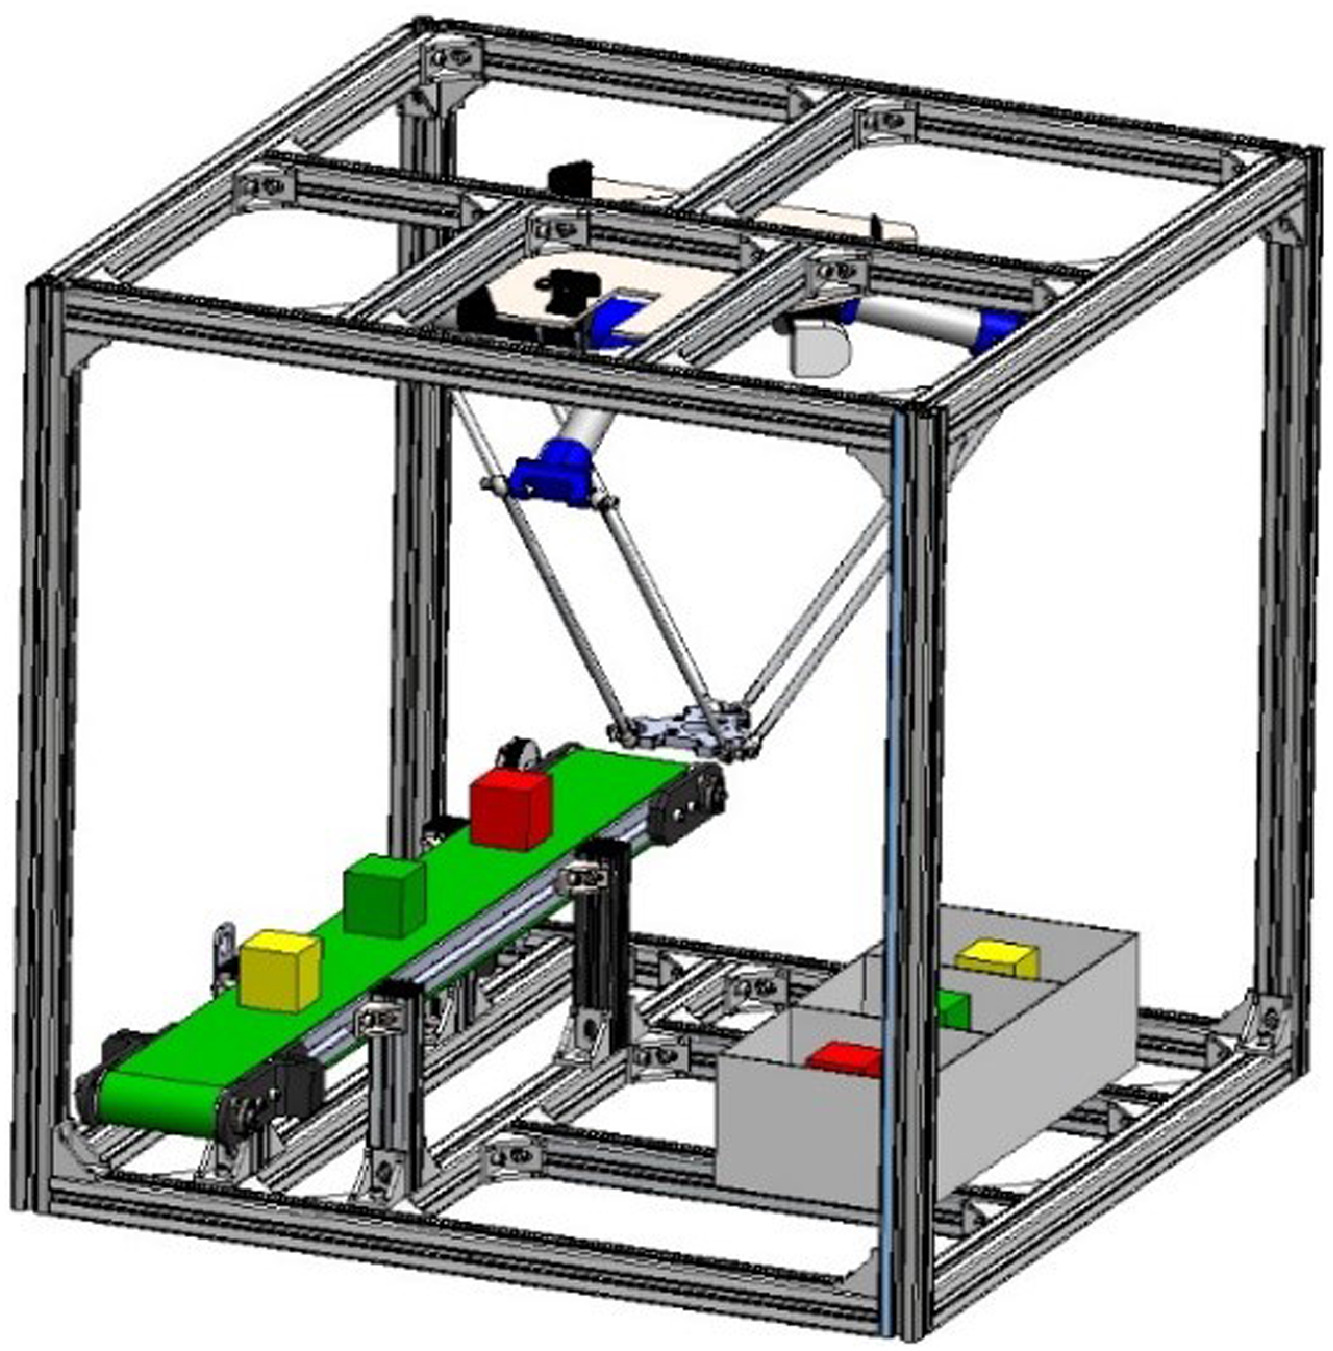
\includegraphics[width=0.5\linewidth]{image/Study Case 3.jpg}
        \caption{Low-cost Delta robot integrated with an HSV-based
                 colour vision system for conveyor-based sorting
                 \autocite{elassal-2024}.}
        \label{fig:case3_image}
    \end{figure}
\end{itemize}

%============================================================================
\subsection{Robot Manipulator}
\hspace{1.27cm}
A robot manipulator is a programmable mechanical system designed to
move objects or tools through space by replicating, in an abstract
sense, the mobility of a biological arm. The system operates through
the coordinated action of joints, connecting links, drive actuators,
and an end-effector, enabling controlled motion across multiple
kinematic axes. In automated production environments these systems
deliver levels of speed, precision, and consistency that are
unattainable by human workers, particularly for tasks that are
physically demanding, environmentally hazardous, or require
sub-millimetre repeatability. Their principal technical strength is
adaptability: by varying the number of joints and the nature of the
actuators, engineers can configure a manipulator that is equally
suited to delicate microsurgery and to handling multi-hundred-kilogram
automotive subassemblies. Achieving the required motion quality demands
real-time computation of joint trajectories and the application of
inverse kinematics algorithms that translate a desired tool-centre-point
position into the corresponding set of joint coordinates.\par
\hspace{1.27cm}
Understanding the architecture of a robot manipulator begins with
its constituent mechanical elements. Three fundamental building
blocks are present in virtually every design: a base structure that
anchors the system to its environment, a series of rigid links that
define the kinematic chain, and the joints that interconnect those
links and provide the system's degrees of freedom.

%============================================================================
\subsubsection{Base}
\hspace{1.27cm}
The base is the structural anchor of the entire manipulator assembly.
Its mechanical role is to absorb the static weight of the arm, the
dynamic loads generated during motion, and any reaction forces
transmitted through the end-effector during contact tasks, without
undergoing meaningful deflection or displacement. In fixed
installations such as assembly lines or machining cells, the base is
bolted directly to a reinforced floor surface or to a rigid support
structure, ensuring that the geometric relationship between the robot
and its work environment remains constant throughout operation. Where
the application requires the manipulator to relocate between multiple
work stations, as in some flexible manufacturing systems, the base may
be mounted on a guided rail, a wheeled carriage, or a tracked platform
that provides controlled translational mobility.

%============================================================================
\subsubsection{Links}
\hspace{1.27cm}
Links are the rigid structural members that form the physical body of
the kinematic chain, connecting each joint to the next and ultimately
carrying the end-effector to its target position. The dimensional
and material properties of the links have a direct bearing on the
robot's key performance characteristics. A longer link extends the
robot's reach and increases the volume of its reachable workspace,
but the additional span introduces greater bending compliance under
load, which degrades positioning accuracy at the tip. Shorter links
offer the inverse trade-off: higher structural stiffness and improved
positional fidelity, at the cost of a reduced working envelope.
Designers also face a choice between structural materials: aluminium
alloys and carbon-fibre composites are favoured where minimising
moving mass is the priority, as lower inertia allows faster
accelerations and reduces actuator power demands; steel and other
high-strength metals are selected for heavy-duty platforms where load
capacity and rigidity take precedence over speed.

%============================================================================
\subsubsection{Joints}
\hspace{1.27cm}
Joints are the kinematic elements that connect consecutive links and
define the nature and range of relative motion between them. The
type of joint used at each location in the chain determines both the
direction and the degree of freedom it contributes to the overall
mechanism. Six principal joint types appear in the robotics literature:

\begin{itemize}
    \item \textbf{Revolute Joints}: This joint type permits only
    rotational motion between the two connected bodies about a single
    fixed axis, providing exactly one degree of freedom. Translation
    along any direction is fully constrained. Revolute joints are the
    most prevalent joint type in industrial manipulators.

    \item \textbf{Prismatic Joints}: A prismatic joint allows one
    body to translate relative to the other along a fixed linear axis
    while completely preventing any rotational motion. It too
    contributes exactly one degree of freedom and is commonly
    encountered in the vertical columns of Cartesian and SCARA robots.

    \item \textbf{Helical Joints}: In a helical joint the rotational
    and translational motions are geometrically coupled so that a
    fixed angular displacement always produces a proportional linear
    displacement. Despite this coupling the mechanism possesses only
    one independent degree of freedom. The principle is identical to
    that of a screw thread and is exploited in lead-screw drive
    systems.

    \item \textbf{Cylindrical Joints}: This joint independently
    permits both rotation about and translation along the same axis,
    contributing two degrees of freedom to the mechanism. The axis of
    the joint defines the common direction for both motions.

    \item \textbf{Universal Joints}: A universal joint, also referred
    to as a U-joint or Cardan joint, links two shafts whose
    longitudinal axes meet at an angle and allows the transmission of
    rotary motion between them. The construction uses two single-axis
    hinges arranged at $90^{\circ}$ to each other and connected by
    a cross-member. Because the output shaft velocity fluctuates
    with shaft angle, this joint does not maintain a constant
    velocity ratio.

    \item \textbf{Spherical Joints}: A spherical or ball-and-socket
    joint provides three independent rotational degrees of freedom
    about the centre of the ball, allowing the connected link to
    assume any angular orientation relative to its neighbour. This
    arrangement is mechanically analogous to the human hip or
    shoulder joint and appears in the forearm linkages of Delta
    robots.
\end{itemize}

\begin{figure}[h]
    \centering
    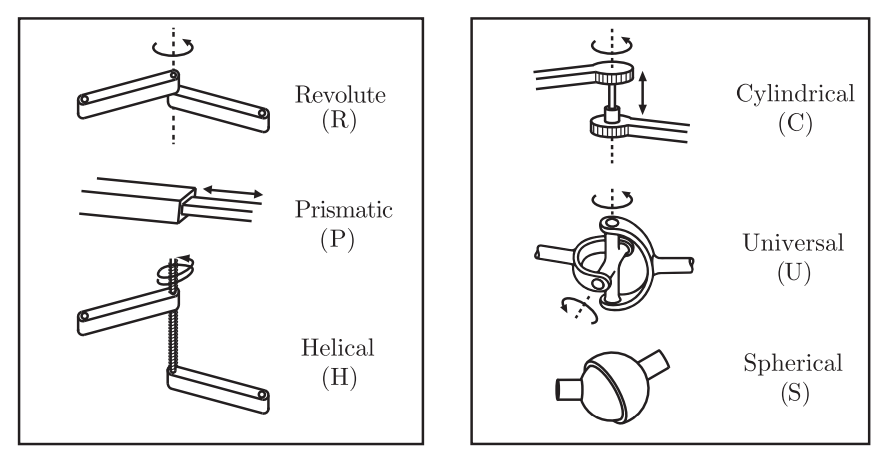
\includegraphics[width=0.8\linewidth]{image/robot_joints.png}
    \caption{Types of Robot Joint.}
    \label{fig:robot_joints}
\end{figure}

\hspace{1.27cm}
The aggregate degrees of freedom of a manipulator equals the sum of
the freedoms contributed by all its joints. A six-revolute-joint arm,
for example, possesses six independent DOF, giving its end-effector
the ability to reach any position and assume any orientation within
the reachable workspace, matching the mobility of a human arm. A
three-joint mechanism has a correspondingly simpler and more
constrained motion space, but this reduced complexity is often
advantageous in high-speed repetitive tasks such as pick-and-place.

%============================================================================
\subsection{Types of Manipulator Robot}

\subsubsection{Cartesian Manipulator Robots}
\hspace{1.27cm}
A Cartesian robot achieves end-effector motion exclusively through
independent linear translation along three mutually orthogonal axes,
each labelled $X$, $Y$, and $Z$ in correspondence with the standard
Cartesian coordinate system. Since each axis of motion is independent
and rectilinear, the kinematic equations governing the system are
relatively uncomplicated, making control system design and real-time
trajectory computation straightforward. This architecture excels in
applications requiring high geometric accuracy and excellent
repeatability, since positioning errors do not accumulate across
joints as they can in rotary-joint chains. The structural frame is
highly modular: standard aluminium extrusion and linear guide
profiles allow workspace volume to be scaled by adjusting the stroke
length of any axis. The rigidity of the gantry structure also
suppresses deflection and vibration when the robot operates over
large areas. Conversely, the rectilinear construction imposes
limitations: the end-effector cannot rotate, so wrist articulation
must be provided by supplementary mechanisms, and the machine
footprint grows in direct proportion to the required workspace
dimensions \autocite{sanchez-sanchez-2010}.\par
\begin{figure}[h]
    \centering
    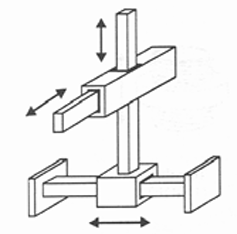
\includegraphics[width=0.5\linewidth]{image/cartesian.png}
    \caption{Cartesian Manipulator Robot.}
    \label{fig:cartesian_manipulator}
\end{figure}
\hspace{1.27cm}
Typical deployment environments for Cartesian robots include
automated assembly lines, computer numerical control (CNC) pick-and-
place machines, material handling gantries, and additive manufacturing
platforms such as 3D printers. Their combination of straightforward
control, scalable workspace, and high positional fidelity makes them
a practical choice wherever linear motion at speed and precision is
the dominant requirement.

%============================================================================
\subsubsection{Cylindrical Manipulator Robots}
\hspace{1.27cm}
A cylindrical manipulator defines its working volume in cylindrical
coordinates rather than Cartesian ones, producing a workspace that
resembles a hollow cylinder or annular region swept around a
vertical axis. The mechanical structure consists of three kinematic
elements: a revolute base joint that rotates the entire arm assembly
about the vertical axis, a prismatic joint that raises and lowers
the arm along that axis, and a second prismatic joint that extends
the arm radially outward or retracts it toward the axis. Together
these three joints provide access to any point within the
characteristic cylindrical shell without requiring the robot to
reorient its base.\par
\hspace{1.27cm}
This configuration offers several operational benefits:
\begin{itemize}
    \item A compact installation envelope suitable for tasks arranged
    around a central work area.
    \item The ability to combine angular sweep with independent linear
    extension, allowing workpieces at varying radial distances to be
    reached without reconfiguring the robot.
    \item Decoupled axis control that simplifies motion programming
    compared to fully rotary configurations.
\end{itemize}
The primary performance limitation is that the rotary base joint
introduces a degree of mechanical backlash that reduces end-effector
positioning accuracy relative to purely linear systems. Additionally,
the workspace does not extend to positions directly above the robot
base or to positions that require motion outside the defined
angular and radial limits, constraining the system's utility in
applications that demand full three-dimensional reachability
\autocite{10629493}.\par
\begin{figure}[h]
    \centering
    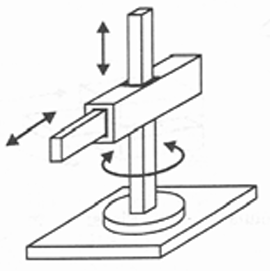
\includegraphics[width=0.5\linewidth]{image/cylindrical.png}
    \caption{Cylindrical Manipulator Robot.}
    \label{fig:cylindrical_manipulator}
\end{figure}
\hspace{1.27cm}
Industrial applications well matched to the cylindrical robot's
workspace geometry include loading and unloading machine tools,
transferring components between radially arranged workstations,
performing spot welds on circular weldments, and stacking items
vertically within a fixed horizontal footprint.

%============================================================================
\subsubsection{Spherical Manipulator Robots}
\hspace{1.27cm}
A spherical manipulator maps its motion capability onto spherical
coordinates, generating a workspace that approximates a partial
hollow sphere centred on the base. The kinematic chain comprises two
revolute joints, one providing rotation about the vertical base axis
and a second enabling vertical angular swing, together with a single
prismatic joint that telescopes the arm radially to adjust reach
distance. This arrangement allows the end-effector to be directed
toward nearly any point on the interior surface of the spherical
shell without requiring extensive base repositioning.\par
\hspace{1.27cm}
According to \autocite{1643416}, this architecture achieves a
favourable compromise between the volume of the accessible workspace
and the mechanical complexity of the structure. The capacity to swing
the arm vertically through a large arc makes spherical robots
particularly effective for tasks requiring access to positions above,
beside, or partially below the robot base, including operations
performed around large workpieces or through access openings. Compared
to Cartesian or cylindrical designs, the spherical robot provides
broader spatial coverage from a single mounting location, though at
the cost of more complex kinematic relationships that complicate
trajectory computation and limit the attainable absolute positioning
accuracy.\par
\begin{figure}[h]
    \centering
    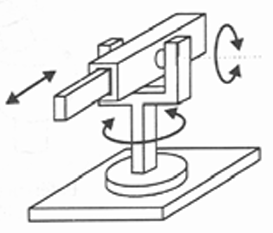
\includegraphics[width=0.5\linewidth]{image/spherical.png}
    \caption{Spherical Manipulator Robot.}
    \label{fig:spherical_manipulator}
\end{figure}
\hspace{1.27cm}
Spherical robots are predominantly deployed in applications where the
broad sweep of the workspace geometry provides operational value and
where end-effector orientation precision is a secondary requirement,
such as arc welding around large structural members, bulk material
transfer, die casting extraction, and machine tool tending.

%============================================================================
\subsubsection{Articulated Manipulator Robots}
\hspace{1.27cm}
Articulated manipulators are constructed as an open serial chain of
rigid links interconnected exclusively by revolute joints, producing
a kinematic topology that closely mirrors the anatomy of the human
upper limb. Commercial designs most commonly incorporate between four
and six such joints, with the six-joint variant providing full
six-degree-of-freedom control over both the position and orientation
of the end-effector. According to \autocite{parhi2012forward}, the
defining mechanical advantage of the articulated configuration is the
combination of a large reachable workspace with an ability to
approach any point within that workspace from multiple orientations,
a flexibility that exceeds what is achievable with Cartesian,
cylindrical, or spherical geometries. The ability to fold the arm
segments close to the body also allows the robot to reach into
confined spaces and around obstacles that would obstruct a less
agile mechanism.\par
\hspace{1.27cm}
These capabilities make articulated robots the configuration of
choice for tasks combining precise positioning with complex
tool-path control, including gas-metal arc welding, robotic painting,
precision component assembly, and camera-guided manipulation. The
technical challenges associated with articulated designs stem from
the nonlinear and coupled nature of the kinematic and dynamic
equations: inverse kinematics solutions are computationally
demanding, and errors in joint angle measurement or mechanical
backlash at any joint propagate through the chain and amplify at
the tip. Real-time compensation for these effects requires careful
attention to controller design and calibration.\par
\begin{figure}[h]
    \centering
    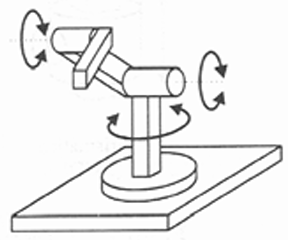
\includegraphics[width=0.5\linewidth]{image/articulated.png}
    \caption{Articulated Manipulator Robot.}
    \label{fig:articulated_manipulator}
\end{figure}
\hspace{1.27cm}
Articulated manipulators are in service across a broad spectrum of
manufacturing sectors, including automotive body-shop welding,
aerospace composite layup, consumer electronics assembly, and
pharmaceutical processing, wherever the simultaneous demand for a
large workspace, high positional accuracy, and flexible orientation
control justifies the investment in a more mechanically and
computationally complex platform.

%============================================================================
\subsubsection{SCARA Manipulator Robots}
\hspace{1.27cm}
The Selective Compliance Assembly Robot Arm, universally identified
by the acronym SCARA, was conceived by Professor Hiroshi Makino at
Yamanashi University during the early 1980s to address the specific
requirements of electronic component assembly: fast horizontal
positioning, precise vertical insertion, and controllable lateral
compliance. The mechanical architecture achieves these goals through
two horizontal revolute joints that sweep the arm through the $XY$
plane, a prismatic joint that drives the end-effector vertically,
and a fourth rotary axis at the wrist that sets tool orientation.
The selective compliance characteristic arises naturally from this
geometry: the arm is intentionally flexible in the horizontal plane,
allowing slight positional corrections during insertion tasks, but
rigid along the vertical $Z$-axis so that downward assembly forces
are resisted without deflection.
\begin{figure}[h]
    \centering
    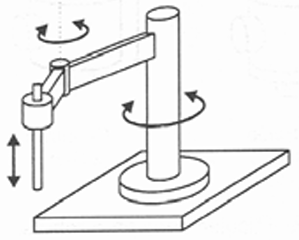
\includegraphics[width=0.5\linewidth]{image/scara.png}
    \caption{SCARA Manipulator Robot.}
    \label{fig:scara_manipulator}
\end{figure}
\par
\hspace{1.27cm}
In production environments SCARA robots are valued for their ability
to execute horizontal pick-and-place cycles at very high throughput.
Commercially available models achieve positional repeatabilities
within $\pm$0.01\,mm and complete single pick-place cycles in under
0.5\,seconds, performance figures that are difficult to match with
other configurations of comparable cost. Principal application domains
include printed circuit board population, pharmaceutical blister
pack loading, small component palletising, and in-process
dimensional inspection. In academic settings the SCARA architecture
is an effective vehicle for teaching kinematic analysis and motion
control because its relatively low degree-of-freedom count and
largely decoupled joint geometry simplify the derivation of both
forward and inverse kinematics solutions.

%============================================================================
\subsubsection{Parallel (Closed-Chain) Manipulator Robots}
\hspace{1.27cm}
A parallel manipulator departs from the conventional serial chain
architecture by connecting the end-effector to the fixed base through
multiple independent kinematic chains that operate simultaneously.
This closed-loop topology distributes the applied load across all
chains in parallel rather than concentrating it in the most distal
joint of a serial chain, producing a structure that is inherently
stiffer, exhibits lower moving inertia, and achieves a higher
ratio of payload capacity to total machine mass compared to
equivalent serial designs \autocite{merlet-2006}. The structural
stiffness of a closed kinematic loop is considerably greater than
that of an open chain of the same mass, and compliance-induced
positioning errors are both reduced in magnitude and more readily
detected and corrected \autocite{merlet-2006}. These mechanical
benefits are accompanied by a more restricted reachable workspace
and significantly more involved kinematic analysis than is required
for serial configurations \autocite{angeles-2004}.\par
\hspace{1.27cm}
A parallel robot may be formally described as a mechanism in which
an end-effector possessing $n$ degrees of freedom is coupled to a
fixed base through a minimum of two independent kinematic chains,
with exactly $n$ independently actuated joints distributed across
those chains \autocite{merlet-2006}. When the count of kinematic
chains equals exactly $n$, the mechanism is termed a fully parallel
manipulator. Three archetypal parallel configurations appear
repeatedly in the literature:
\begin{itemize}
    \item Stewart--Gough Platform: A six-degree-of-freedom
    fully parallel manipulator consisting of a rigid upper platform
    connected to a fixed base plate by six independently actuated
    telescoping struts, each terminating in universal and
    ball-and-socket joints. This architecture underpins the majority
    of six-axis motion simulators and ultra-precision machining
    platforms \autocite{merlet-2006}.
\begin{figure}[h]
    \centering
    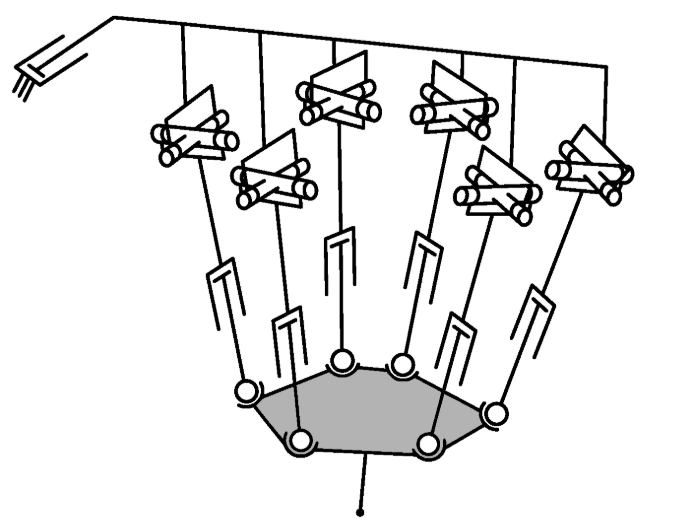
\includegraphics[width=0.5\linewidth]{image/Parallel6DOF.png}
    \caption{A 6-DOF Parallel Manipulator.}
    \label{fig:6DOF_parallel_manipulator}
\end{figure}
    \item Delta Robot: A three-degree-of-freedom
    translational parallel manipulator in which three kinematic
    chains restrict the moving platform to purely translational
    motion. Each chain combines a base-mounted rotary actuator with
    a passive parallelogram forearm. Because all actuators are
    located at the base, the moving mass is minimised, enabling
    cycle times below 0.3\,seconds and establishing this design as
    the standard platform for high-throughput pick-and-place in the
    food, pharmaceutical, and electronics industries
    \autocite{clavel-1990, merlet-2006}.
\end{itemize}
\begin{figure}[h]
    \centering
    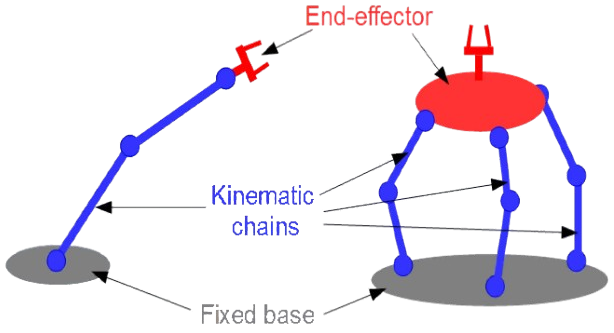
\includegraphics[width=0.5\linewidth]{image/Parallel.png}
    \caption{A 3-DOF Parallel Manipulator.}
    \label{fig:3DOF_Parallel}
\end{figure}

%============================================================================
\subsection{Delta Robot Kinematics}

\subsubsection{Geometric Description}
\hspace{1.27cm}
The geometry of a Delta robot is fully characterised by four
dimensional parameters: the side length $f$ of the equilateral
triangle formed by the fixed base joints, the side length $e$ of
the equilateral triangle formed by the moving platform joints,
the length $r_f$ of each proximal upper arm, and the length $r_e$
of each distal forearm \autocite{mzavatsky-2009}. Together these
four measurements determine the shape and volume of the reachable
workspace and govern the sensitivity of the end-effector position
to changes in joint angle. The origin of the reference coordinate
frame is located at the geometric centre of the fixed base triangle,
and the $z$-axis is directed downward so that every valid
end-effector position is assigned a negative $z$-coordinate.

\begin{figure}[h]
    \centering
    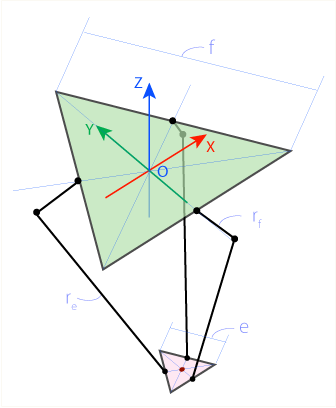
\includegraphics[width=0.4\linewidth]{attachment3.png}
    \caption{Geometric parameters of the Delta robot: fixed base
             side $f$, moving platform side $e$, upper arm $r_f$,
             and forearm $r_e$ \autocite{mzavatsky-2009}.}
    \label{fig:delta_geometry}
\end{figure}

%============================================================================
\subsubsection{Forward Kinematics}
\hspace{1.27cm}
Forward kinematics (FK) addresses the problem of computing the
Cartesian end-effector position $(x_0, y_0, z_0)$ when the three
joint angles $(\theta_1, \theta_2, \theta_3)$ are known, for
example from encoder readings. For the Delta robot the solution
exploits the geometric interpretation of each forearm as the radius
of a sphere: the end-effector must lie simultaneously on three
spheres of radius $r_e$ centred at three adjusted joint positions
$J'_1$, $J'_2$, $J'_3$ derived from the joint angles
\autocite{zsombor-murray-2004}.\par
\hspace{1.27cm}
Pairwise subtraction of the three sphere equations cancels all
second-order terms in $x$ and $y$, leaving two equations that are
linear in the unknowns:

\begin{cequation}
    x_0 = a_1 z_0 + b_1, \qquad y_0 = a_2 z_0 + b_2
    \label{eq:fk_linear}
\end{cequation}

where the scalar coefficients $a_1,\, a_2,\, b_1,\, b_2$ depend
on the coordinates of the adjusted joint centres. Back-substituting
\autoref{eq:fk_linear} into one of the original sphere equations
produces a univariate quadratic equation in $z_0$:

\begin{multline}
    (a_1^2 + a_2^2 + 1)\,z_0^2
    \;+\; 2\bigl[a_1(b_1 - y_1) + a_2(b_2 - y_1) - z_1\bigr]\,z_0
    \;\\ + \; \bigl[(b_1 - y_1)^2 
    + (b_2 - y_1)^2 + z_1^2 -
    r_e^2\bigr] = 0
    \label{eq:fk_quadratic}
\end{multline}

Of the two roots of \autoref{eq:fk_quadratic} the physically
realizable configuration corresponds to the more negative value.
A negative discriminant signals that the supplied joint angles
cannot place the end-effector at any real point in space, indicating
a mechanically invalid configuration \autocite{mzavatsky-2009}. In
the system described in this thesis, FK is not used in the primary
motion-planning loop. Instead it functions as a post-movement
verification tool: after each commanded motion the encoder angles
are fed through FK and the computed position is compared against
the commanded target to identify gross mechanical faults.

%============================================================================
\subsubsection{Inverse Kinematics}
\hspace{1.27cm}
Inverse kinematics (IK) solves the complementary problem: given a
desired end-effector position $(x_0, y_0, z_0)$, find the joint
angle triplet $(\theta_1, \theta_2, \theta_3)$ that realises it.
The three-fold rotational symmetry of the Delta mechanism means
that each limb can be treated as an independent sub-problem
\autocite{mzavatsky-2009}. For the first limb the proximal joint is
mechanically constrained to rotate within the $YZ$ plane, reducing
the spatial three-sphere intersection to a two-circle intersection
problem in that plane.\par
\hspace{1.27cm}
The calculation begins by projecting the relevant end-effector
attachment point $E_1$ onto the $YZ$ plane to obtain $E'_1$. The
angular position of the proximal joint $J_1$ is then determined
as the intersection of a circle of radius $r_f$ centred on the
base attachment point $F_1$ with a circle of radius
$\sqrt{r_e^2 - x_0^2}$ centred on $E'_1$; where two intersections
exist, the geometrically admissible one is that with the smaller
$y$-coordinate. The corresponding joint angle follows from:

\begin{cequation}
    \theta_1 = \arctan\!\left(\frac{z_{J_1}}{y_{F_1} -
    y_{J_1}}\right)
    \label{eq:ik_theta1}
\end{cequation}

The second and third joint angles $\theta_2$ and $\theta_3$ are
computed by applying the same procedure to coordinate frames rotated
by $+120^{\circ}$ and $-120^{\circ}$ about the $Z$-axis
respectively \autocite{zsombor-murray-2004}. Should the
discriminant of the circle-intersection sub-problem be negative
for any limb, the requested position lies outside the reachable
workspace and the motion command must be rejected before any
actuation occurs.

%============================================================================
\subsection{Workspace Analysis}
\hspace{1.27cm}
The reachable workspace of a Delta robot encompasses all
end-effector positions that can be attained without any joint angle
exceeding its physical limit and without the mechanism passing
through a singular configuration. The outer boundary of this volume
approximates a cylinder whose top and bottom faces are bounded by
rounded surfaces determined by the geometric interference between
the kinematic chains. The specific shape and volume of the workspace
are governed primarily by the four geometric parameters $f$, $e$,
$r_f$, and $r_e$, with the actuator joint-angle limits providing
the secondary constraint \autocite{stock-2003}.\par
\hspace{1.27cm}
Accurate workspace knowledge serves two practical purposes in the
present system. First, it establishes the set of robot-frame
coordinates for which the IK solver will return a valid solution;
any object position reported by the vision system that falls outside
this region must be discarded by the safety module before it can
be forwarded to the motion controller. Second, the workspace
boundary provides the spatial reference needed to position the
RealSense D455 camera so that its field of view completely
encompasses the area within which objects can be picked
\autocite{bonev-2001}.

\begin{figure}[h]
    \centering
    \includegraphics[width=0.7\linewidth]{image/Reachable workspace
    of a Delta robot.jpg}
    \caption{Reachable workspace of a Delta robot, approximating a
             cylindrical volume \autocite{stock-2003}.}
    \label{fig:workspace_delta}
\end{figure}

%============================================================================
\subsection{Vision System: Camera and 2D Localisation}

\subsubsection{Intel RealSense D455}
\hspace{1.27cm}
The Intel RealSense D455 is a structured-light stereo camera that
combines a passive infrared stereo imager pair with an active
infrared flood illuminator and a co-located colour sensor. Its
stereo baseline of 95\,mm exceeds that of the D435 model (55\,mm),
providing more stable image acquisition at the operating distance
used in this system \autocite{intel-realsense-d455}. The colour
stream delivers up to 30\,frames per second at resolutions suitable
for real-time object detection, and the associated intrinsic
calibration data including focal lengths $f_x$, $f_y$ and
principal-point coordinates $c_x$, $c_y$ are published
continuously on the \texttt{camera\_info} topic within the ROS~2
graph.

\subsubsection{Pinhole Camera Model}
\hspace{1.27cm}
The imaging geometry of the RealSense D455 colour sensor is
modelled by the standard pinhole projection. A physical point
$\mathbf{P}_c = [X_c,\, Y_c,\, Z_c]^{\top}$ in the camera
coordinate frame projects onto the image plane at pixel
coordinates $(u, v)$ according to \autocite{hartley-2004}:

\begin{cequation}
    \begin{bmatrix} u \\ v \\ 1 \end{bmatrix}
    =
    \frac{1}{Z_c}
    \begin{bmatrix}
        f_x & 0   & c_x \\
        0   & f_y & c_y \\
        0   & 0   & 1
    \end{bmatrix}
    \begin{bmatrix} X_c \\ Y_c \\ Z_c \end{bmatrix}
    =
    \frac{1}{Z_c}\, \mathbf{K}\, \mathbf{P}_c,
    \label{eq:pinhole_matrix}
\end{cequation}

where $\mathbf{K}$ is the $3 \times 3$ camera intrinsic matrix.
Expanding \autoref{eq:pinhole_matrix} gives the familiar
component-wise projection equations:

\begin{cequation}
    u = f_x \cdot \frac{X_c}{Z_c} + c_x,
    \qquad
    v = f_y \cdot \frac{Y_c}{Z_c} + c_y.
    \label{eq:pinhole_uv}
\end{cequation}

The four intrinsic parameters are defined as follows:
$f_x = f / s_x$ and $f_y = f / s_y$, where $f$ is the physical
focal length of the lens and $s_x$, $s_y$ are the horizontal and
vertical pixel pitch of the image sensor; $c_x$ and $c_y$ are the
coordinates of the principal point, ideally located at the image
centre but offset by small manufacturing tolerances.

\subsubsection{2D Localisation via Fixed-Height Backprojection}
\hspace{1.27cm}
Since every target object in this system rests on the conveyor
belt surface at a fixed, pre-measured height below the camera,
the scene depth is not unknown but constant: $Z_c = Z_{\text{belt}}$
for all objects. This constraint eliminates the need for per-frame
depth measurement and allows the full pixel-to-camera-frame
localisation to be performed using only the colour image.

\par
\hspace{1.27cm}
Inverting \autoref{eq:pinhole_uv} under the fixed-depth
assumption yields the camera-frame planar coordinates of a
detected object directly from its pixel centre $(u, v)$:

\begin{cequation}
    X_c = \frac{(u - c_x)\cdot Z_{\text{belt}}}{f_x},
    \qquad
    Y_c = \frac{(v - c_y)\cdot Z_{\text{belt}}}{f_y}.
    \label{eq:backproject}
\end{cequation}

In homogeneous matrix notation, this backprojection can be
written as:

\begin{cequation}
    \begin{bmatrix} X_c \\ Y_c \\ Z_c \end{bmatrix}
    =
    Z_{\text{belt}}\,
    \mathbf{K}^{-1}
    \begin{bmatrix} u \\ v \\ 1 \end{bmatrix}
    =
    Z_{\text{belt}}
    \begin{bmatrix}
        \frac{1}{f_x} & 0              & -\frac{c_x}{f_x} \\[4pt]
        0              & \frac{1}{f_y} & -\frac{c_y}{f_y} \\[4pt]
        0              & 0              & 1
    \end{bmatrix}
    \begin{bmatrix} u \\ v \\ 1 \end{bmatrix}.
    \label{eq:backproject_matrix}
\end{cequation}

The scalar $Z_{\text{belt}}$ is determined once during system
setup as the physically measured vertical distance from the camera
optical centre to the belt surface, and it remains constant
throughout operation. The resulting 3D point
$[X_c,\, Y_c,\, Z_{\text{belt}}]^{\top}$ expressed in the camera
frame is then forwarded to the coordinate frame transformation
stage described in \autoref{sec:coordinate_transform}.

\subsubsection{Intrinsic Parameter Acquisition}
\hspace{1.27cm}
The four intrinsic parameters $f_x$, $f_y$, $c_x$, $c_y$ required
by \autoref{eq:pinhole_matrix} are not hardcoded but are read at
runtime from the \texttt{/camera/color/camera\_info} topic
published by the \texttt{realsense2\_camera} ROS~2 node. The
\texttt{camera\_info} message carries the full $3 \times 3$ intrinsic
matrix $\mathbf{K}$ as a row-major nine-element array. In the
detection node, the parameters are extracted on the first message
receipt and cached for the remainder of the session:

\begin{cequation}
    \mathbf{K} =
    \begin{bmatrix}
        K[0] & 0    & K[2] \\
        0    & K[4] & K[5] \\
        0    & 0    & 1
    \end{bmatrix}
    =
    \begin{bmatrix}
        f_x & 0   & c_x \\
        0   & f_y & c_y \\
        0   & 0   & 1
    \end{bmatrix}.
    \label{eq:K_from_topic}
\end{cequation}

Reading $\mathbf{K}$ from the live topic rather than a static
configuration file ensures that the correct parameters are used
regardless of any change in camera resolution or mounting, since
the RealSense driver recomputes and publishes the intrinsics
appropriate to the active stream profile on every startup.

%============================================================================
\subsection{Coordinate Frame Transformation}
\hspace{1.27cm}
Once the image-plane position of a detected object has been
determined, it must be expressed in the robot base frame before
it can serve as an input to the inverse kinematics solver. This
mapping is a rigid-body transformation — commonly referred to
as hand-eye calibration — that encodes the fixed geometric
relationship between the camera coordinate frame and the robot
base frame. The general form of the transformation is a
homogeneous matrix $\mathbf{H}$ comprising a $3 \times 3$
rotation matrix $\mathbf{R}$ and a $3 \times 1$ translation
vector $\mathbf{T}$:

\begin{cequation}
    \mathbf{H} =
    \begin{bmatrix}
        \mathbf{R} & \mathbf{T} \\
        \mathbf{0}^{\top} & 1
    \end{bmatrix},
    \label{eq:homogeneous}
\end{cequation}

so that a point $\mathbf{p}_c = [X_c,\, Y_c,\, Z_c,\, 1]^{\top}$
expressed in the camera frame is mapped to the robot base frame
as:

\begin{cequation}
    \begin{bmatrix} X_r \\ Y_r \\ Z_r \\ 1 \end{bmatrix}
    =
    \begin{bmatrix}
        \mathbf{R} & \mathbf{T} \\
        \mathbf{0}^{\top} & 1
    \end{bmatrix}
    \begin{bmatrix} X_c \\ Y_c \\ Z_c \\ 1 \end{bmatrix}
    =
    \mathbf{R}
    \begin{bmatrix} X_c \\ Y_c \\ Z_c \end{bmatrix}
    + \mathbf{T}.
    \label{eq:transform}
\end{cequation}

\hspace{1.27cm}
The rotation matrix $\mathbf{R}$ is a $3 \times 3$ orthonormal
matrix of the first kind ($\det(\mathbf{R}) = 1$) that encodes
the angular orientation of the camera frame relative to the robot
base frame. Any such rotation can be parameterised by a unit
axis vector $\hat{n} = [n_1,\, n_2,\, n_3]^{\top}$ and a
rotation angle $\theta$ through the Rodrigues formula
\autocite{tsai-lenz-1989}:

\begin{multline}
    \mathbf{R} =
    \begin{bmatrix}
        n_1^2 + (1-n_1^2)\cos\theta &
        n_1 n_2(1-\cos\theta) - n_3\sin\theta &
        n_1 n_3(1-\cos\theta) + n_2\sin\theta \\[4pt]
        n_1 n_2(1-\cos\theta) + n_3\sin\theta &
        n_2^2 + (1-n_2^2)\cos\theta &
        n_2 n_3(1-\cos\theta) - n_1\sin\theta \\[4pt]
        n_1 n_3(1-\cos\theta) - n_2\sin\theta &
        n_2 n_3(1-\cos\theta) + n_1\sin\theta &
        n_3^2 + (1-n_3^2)\cos\theta
    \end{bmatrix}.
    \label{eq:rodrigues}
\end{multline}

The translation vector $\mathbf{T} = [t_x,\, t_y,\, t_z]^{\top}$
encodes the position of the camera optical centre expressed in
the robot base frame, accounting for the physical mounting offset
of the camera relative to the robot origin.

\subsubsection{Coordinate Frame Definitions}
\hspace{1.27cm}
Following the notation of \autocite{tsai-lenz-1989}, four
coordinate frames are relevant to the transformation:

\begin{itemize}
    \item $\mathcal{F}_r$ : the robot base frame,
    fixed at the kinematic origin of the robot. All motor commands
    and IK inputs are expressed in this frame.
    \item $\mathcal{F}_c$ : the camera frame, centred
    at the camera optical centre with the $z$-axis coinciding
    with the optical axis and the $x$- and $y$-axes aligned with
    the image plane horizontal and vertical directions,
    respectively.
    \item $\mathcal{F}_w$ : the calibration world frame,
    an auxiliary frame defined on the calibration target at known
    positions during the calibration procedure.
    \item $\mathcal{F}_b$ : the belt (object) frame,
    the plane in which detected objects reside, at a fixed and
    measured height $Z_{\text{fixed}}$ below $\mathcal{F}_r$.
\end{itemize}

\subsubsection{Calibration Procedure}
\hspace{1.27cm}
The process of determining $\mathbf{R}$ and $\mathbf{T}$ is
known as \textit{eye-to-hand calibration} when the camera is
mounted at a fixed location in the workspace rather than on the
robot arm. Tsai and Lenz \autocite{tsai-lenz-1989} showed that
this relationship can be recovered from a set of corresponding
point observations without requiring global nonlinear
optimisation: the problem decomposes into first solving for the
rotation $\mathbf{R}$ via a linear least-squares system, and
subsequently solving for the translation $\mathbf{T}$ from a
second linear system given the already-determined $\mathbf{R}$.
The minimum number of calibration stations required for a unique
solution is three \autocite{tsai-lenz-1989}.

\par
\hspace{1.27cm}
In this system, an empirical axis-alignment calibration procedure
is adopted, following the physical verification approach. The
procedure is carried out in four sequential steps:

\begin{enumerate}
    \item Origin alignment: A reference object is placed
    at the geometric centre of the robot workspace, where
    $X_r \approx 0$ and $Y_r \approx 0$ by definition. The
    translation offsets $t_x$ and $t_y$ in $\mathbf{T}$ are
    adjusted until the reported robot-frame coordinates of the
    detected object match the known physical position.

    \item Axis sign and assignment verification: The
    object is displaced in the positive $X_r$ direction by a
    known distance $\Delta x$. If the reported coordinate
    increases accordingly, the $X$ axis mapping is confirmed.
    If it decreases, the sign of the corresponding column of
    $\mathbf{R}$ is negated. The same test is repeated for the
    $Y_r$ direction.

    \item Scale validation: The object is moved to a
    set of positions at known metric distances from the origin.
    The Euclidean error between the reported and measured
    positions is computed. If errors exceed the acceptable
    threshold, the focal-length and principal-point parameters
    used in the projection are re-verified against the live
    \texttt{camera\_info} topic.

    \item Full-workspace validation: The object is
    placed at five or more positions distributed across the
    robot workspace. The mean and maximum absolute errors in
    $X_r$ and $Y_r$ are recorded. Calibration is accepted when
    the mean error is below 5\,mm across all test positions.
\end{enumerate}

\subsubsection{Transformation Matrix Construction}
\hspace{1.27cm}
For the fixed eye-to-hand mounting geometry used in this system,
the camera is positioned above the workspace with its optical
axis directed downward and slightly offset from the robot
base-frame origin. The rotation matrix $\mathbf{R}$ encodes two
effects: the physical angular mounting of the camera (roll,
pitch, yaw relative to the robot frame) and the axis convention
difference between the camera frame (where $y$ points downward
in the image) and the robot frame (where $Y$ points in the
robot's forward direction). In practice, $\mathbf{R}$ takes the
form of a sign-permutation matrix with possible negations,
determined through the axis verification procedure described
above. Once the calibration is complete, the full transformation
from a detected pixel centre $(u, v)$ to robot base-frame
coordinates $(X_r, Y_r)$ is:

\begin{cequation}
    \begin{bmatrix} X_r \\ Y_r \end{bmatrix}
    =
    \mathbf{R}_{2 \times 2}
    \begin{bmatrix} X_c \\ Y_c \end{bmatrix}
    +
    \begin{bmatrix} t_x \\ t_y \end{bmatrix},
    \label{eq:transform_2d}
\end{cequation}

where $X_c$ and $Y_c$ are the camera-frame coordinates derived
from the pixel observation and the known belt height
$Z_{\text{fixed}}$, and $\mathbf{R}_{2 \times 2}$ is the
upper-left $2 \times 2$ submatrix of $\mathbf{R}$ applicable to
the planar constraint. The vertical robot coordinate $Z_r$ is
not computed from the camera but is set to the fixed pick height
$Z_{\text{pick}}$ measured during system setup, consistent with
the flat-world assumption that all target objects rest on the
belt surface at a constant elevation.

%============================================================================
\subsection{Object Detection: YOLO}
\hspace{1.27cm}
You Only Look Once (YOLO) refers to a line of single-stage
convolutional neural network architectures in which object
detection is formulated as a direct regression from the input
image to a set of bounding box parameters and class probability
vectors, with the entire computation performed in a single
forward pass through the network \autocite{redmon-2016}. By
eliminating the region-proposal stage that is characteristic of
two-stage detectors such as Faster R-CNN, YOLO achieves inference
latencies that are well suited to closed-loop robotic systems
where the speed of the detection result directly limits the
achievable control bandwidth.

\begin{figure}[h]
    \centering
    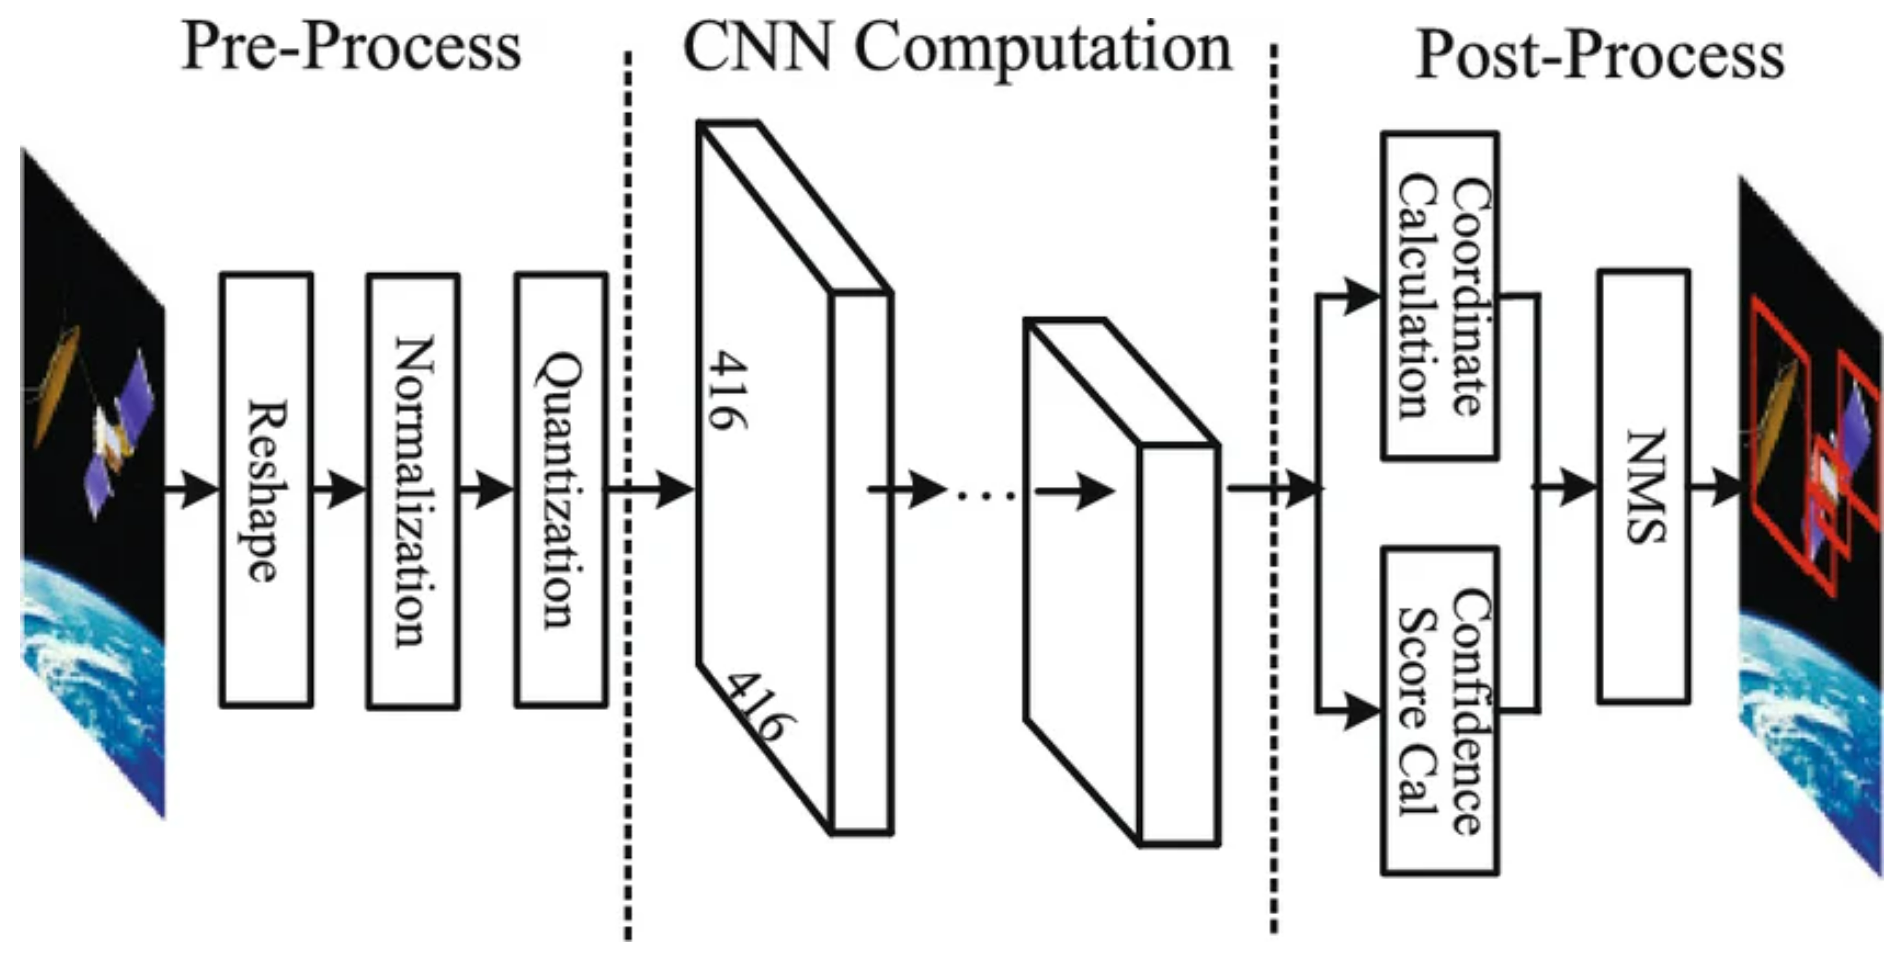
\includegraphics[width=0.7\linewidth]{image/Architecture of the YOLO network.png}
    \caption{Architecture of The YOLO Network \autocite{redmon-2016}.}
    \label{fig:YOLO architecure}
\end{figure}



\par
\hspace{1.27cm}
The family has evolved through multiple generations, from the
original network through YOLOv5, YOLOv7, YOLOv8, and the YOLO11
series, each introducing architectural refinements that improve
the precision-recall curve and reduce inference time on embedded
GPU hardware \autocite{jocher-2023}. In pick-and-place
applications, the centroid $(u, v)$ of the bounding box returned
by the detector is taken as the pixel-plane position of the
target object and forwarded to the coordinate transformation
stage.

%============================================================================
\subsection{Trajectory Planning and Control}
\hspace{1.27cm}
Trajectory planning is the process of computing a
time-parameterised sequence of end-effector positions,
velocities, and accelerations that connects an initial
configuration to a goal configuration while simultaneously
satisfying the velocity, acceleration, and jerk constraints
imposed by the physical actuators and the structural dynamics
of the mechanism \autocite{biagiotti-2008}. For Delta robots,
where the moving platform is extremely lightweight and the
parallel linkages exhibit low structural damping, trajectory
quality has a direct and measurable effect on placement
accuracy: a poorly shaped motion profile excites the natural
resonance modes of the linkage structure, producing residual
oscillations at the end-effector that persist after the
nominal motion has ended and degrade pick-and-place
repeatability \autocite{siciliano-2009}.

\subsubsection{Joint-Space and Cartesian-Space Planning}
\hspace{1.27cm}
Trajectory planning for robotic manipulators can be performed
either in joint space or in Cartesian space, and the choice
has practical consequences for path predictability and
computational load \autocite{siciliano-2009}. In
joint-space planning, a smooth scalar function
$\theta_i(t)$ is constructed independently for each joint
angle between its initial and final values. The resulting
end-effector path in Cartesian space is not a straight line
but follows whatever curve the forward kinematics maps the
joint interpolation onto. However, joint-space planning
guarantees that velocity and acceleration limits are satisfied
by construction and avoids continuous IK evaluations during
motion execution. In Cartesian-space planning, the
desired end-effector position
$\mathbf{p}(t) = [x(t),\, y(t),\, z(t)]^{\top}$ is defined
directly as a function of time, and the IK solver is invoked
at every control step to convert the Cartesian setpoint to
joint coordinates. This approach produces geometrically
predictable straight-line or curved paths at the cost of
continuous IK computation and increased risk of encountering
workspace boundaries or kinematic singularities mid-trajectory
\autocite{biagiotti-2008}.

\subsubsection{Polynomial Velocity Profiles}
\hspace{1.27cm}
Regardless of whether planning is performed in joint space or
Cartesian space, a time-scaling function $s(t)$ is used to
shape the velocity and acceleration profiles of each motion
segment. Two profile forms are widely used in the robotics
literature \autocite{biagiotti-2008}.

\par
\hspace{1.27cm}
\begin{itemize}
    \item Trapezoidal profile is divided into three phases, a constant-acceleration phase of duration $t_a$, a
constant-velocity cruise phase, and a symmetric
constant-deceleration phase. The velocity profile is:
\end{itemize}


\begin{cequation}
    \dot{s}(t) =
    \begin{cases}
        \dfrac{v_{\max}}{t_a}\, t,
            & 0 \leq t < t_a \\[6pt]
        v_{\max},
            & t_a \leq t \leq T - t_a \\[6pt]
        \dfrac{v_{\max}}{t_a}(T - t),
            & T - t_a < t \leq T
    \end{cases}
    \label{eq:trap_vel}
\end{cequation}

where $v_{\max}$ is the peak velocity and $T$ is the total
segment duration. The acceleration is piecewise constant at
$\pm v_{\max}/t_a$, meaning the jerk at the phase transition
points is theoretically unbounded. For high-speed lightweight
mechanisms such as Delta robots, this jerk discontinuity
excites structural resonance and causes residual vibration at
the end-effector \autocite{siciliano-2009}.

\par
\hspace{1.27cm}
\begin{itemize}
\item Quintic polynomial profile is a degree-five polynomial
satisfying boundary conditions of zero displacement error,
zero velocity, and zero acceleration at both the start and
end of the segment provides continuity through the second
derivative, eliminating the jerk discontinuity of the
trapezoidal profile \autocite{biagiotti-2008}. Using the
normalised time variable $\tau = t/T \in [0, 1]$, the profile
is:
\end{itemize}
\begin{cequation}
    s(\tau) = 10\tau^3 - 15\tau^4 + 6\tau^5,
    \label{eq:quintic}
\end{cequation}

with velocity and acceleration:

\begin{cequation}
    \dot{s}(\tau) = \frac{1}{T}
    \left(30\tau^2 - 60\tau^3 + 30\tau^4\right),
    \label{eq:quintic_vel}
\end{cequation}

\begin{cequation}
    \ddot{s}(\tau) = \frac{1}{T^2}
    \left(60\tau - 180\tau^2 + 120\tau^3\right).
    \label{eq:quintic_acc}
\end{cequation}

The smooth bell-shaped velocity profile and the continuous
acceleration curve of
\autoref{eq:quintic}--\autoref{eq:quintic_acc} suppress
structural excitation and make the quintic polynomial the
preferred time-scaling function for lightweight parallel
manipulators where residual vibration is the dominant source
of placement error \autocite{biagiotti-2008}.

\subsubsection{Actuator-Level Control}
\hspace{1.27cm}
At the actuator level, modern brushless servo motors and
quasi-direct-drive (QDD) actuators typically implement an
onboard PD position controller that closes the position loop
at high frequency independently of the host computer. The
general form of the torque command is \autocite{siciliano-2009}:

\begin{cequation}
    \tau = K_p\,(\theta_{\text{des}} - \theta_{\text{enc}})
         + K_d\,(\dot{\theta}_{\text{des}} -
         \dot{\theta}_{\text{enc}}),
    \label{eq:pd_control}
\end{cequation}

where $\tau$ is the output torque, $\theta_{\text{des}}$ and
$\dot{\theta}_{\text{des}}$ are the desired position and
velocity set-points, $\theta_{\text{enc}}$ and
$\dot{\theta}_{\text{enc}}$ are the encoder-measured position
and velocity, and $K_p$, $K_d$ are the proportional and
derivative gains. When this local control loop is combined with
a supervisory Cartesian trajectory planner operating in
real-time, the overall architecture separates motion shaping
from position regulation: the planner is responsible for
producing smooth, dynamically feasible set-points, while the
onboard controller is responsible for tracking those set-points
accurately despite actuator dynamics and disturbances
\autocite{siciliano-2009}.

\subsubsection{Forward Kinematics Validation}
\hspace{1.27cm}
In closed-loop motion control of parallel robots, it is
standard practice to verify the actual end-effector position
after each commanded motion by reading the joint encoder values
and applying the forward kinematics model \autocite{merlet-2006}.
This post-motion validation step detects discrepancies between
the commanded and achieved positions that may result from
mechanical compliance, actuator saturation, or CAN communication
faults. If the Euclidean error between the FK-computed position
and the commanded target exceeds a defined threshold, the
controller can halt the motion sequence, trigger a fault
response, and return the robot to a safe home position before
the next pick cycle begins. This validation approach is
particularly important in vision-guided systems, where an
uncorrected positioning error in one cycle can compound with
a subsequent detection error in the next \autocite{yamtuan-2023}.

%============================================================================
\subsection{Pick-and-Place Operation}
\hspace{1.27cm}
Pick-and-place represents the core operational sequence for which
the Delta robot was originally designed and remains its dominant
industrial application \autocite{biagiotti-2008}. A complete
cycle is decomposed into four sequential motion phases, each
defined by a set of Cartesian waypoints:

\begin{enumerate}
    \item Approach: Starting from the home configuration,
    the end-effector travels horizontally to a position vertically
    above the target object while maintaining a safety clearance
    height that prevents any contact with the work surface.

    \item Descend and Grasp: The end-effector descends
    vertically to the object surface elevation and the gripper
    (pneumatic suction cup or mechanical jaw) is actuated to
    secure the object.

    \item Lift and Transfer: The end-effector retracts
    vertically to the safety clearance height with the object
    held securely, then translates horizontally to the designated
    placement location along a smoothly profiled trajectory.

    \item Place and Release: The end-effector descends
    to the placement elevation, the gripper releases, and the
    robot returns to the home position in preparation for the
    next detection cycle.
\end{enumerate}

\hspace{1.27cm}
Each Cartesian waypoint in the above sequence is individually
validated by the IK solver before execution begins. Any waypoint
that maps to a configuration outside the reachable workspace
triggers an immediate abort, returning the robot to the home
position without attempting the motion \autocite{yamtuan-2023}.

%============================================================================
\subsection{Key Control and Software}

\subsubsection{Robot Operating System 2 (ROS~2)}
\hspace{1.27cm}
ROS~2 is an open-source distributed robotics middleware framework
developed as a ground-up redesign of the original ROS~1
infrastructure, addressing limitations that became apparent as
ROS~1 was deployed in safety-critical and multi-robot industrial
applications \autocite{ros2-2022}. The most significant
architectural departure from its predecessor is the adoption of
the Data Distribution Service (DDS) standard as the underlying
communication layer. DDS provides a fully decentralised,
broker-free publish-subscribe transport that supports deterministic
delivery guarantees, configurable Quality of Service (QoS) policies
for controlling message priority, reliability, and latency, and
native inter-process as well as intra-process communication
without requiring a central master process.\par
\begin{figure}[h]
    \centering
    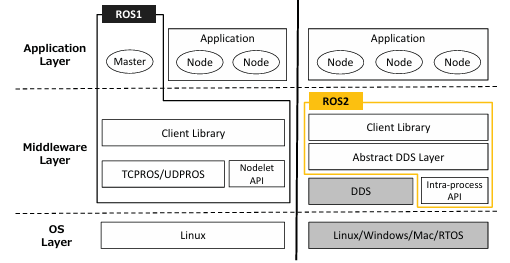
\includegraphics[width=0.7\linewidth]{image/ros2 art.png}
    \caption{ROS~2 Layered Software Architecture.}
    \label{fig:ROS2_Architecture}
\end{figure}
\hspace{1.27cm}
The layered structure of ROS~2, shown in
\textbf{\autoref{fig:ROS2_Architecture}}, positions user
application nodes at the top tier. Developers write these nodes
in C++ using the \texttt{rclcpp} client library or in Python using
\texttt{rclpy}, both of which expose an identical set of
communication primitives so that subsystems written in different
languages can interoperate transparently. These client libraries
issue calls to an abstract DDS interface layer that insulates
application code from the specifics of the DDS vendor in use,
and below this layer the chosen DDS implementation handles
all message serialisation, transport, and delivery. The lowest
tier is the host operating system; ROS~2 runs on Linux, Windows,
and macOS, and a real-time profile enables deployment on RTOS
kernels where deterministic scheduling latency is required.

%============================================================================
\subsubsection{CAN Bus}
\hspace{1.27cm}
The Controller Area Network (CAN) protocol is a differential-pair
serial bus standard originally developed by Bosch for use in
automotive electronic control systems and subsequently adopted
as the preferred intra-machine communication medium for industrial
robot drives \autocite{bosch-can-1991}. Its appeal in robotics
applications derives from a combination of high noise immunity on
the differential signal pair, non-destructive bitwise
priority-based bus arbitration that avoids data collisions, and
deterministic message latency at data rates of up to 1\,Mbit/s
for classic CAN or up to 8\,Mbit/s for the newer CAN~FD variant.
These properties allow motor controllers distributed around the
robot arm to be polled and updated at rates of several hundred
hertz over a single two-wire cable.\par

\begin{figure}[h]
    \centering
    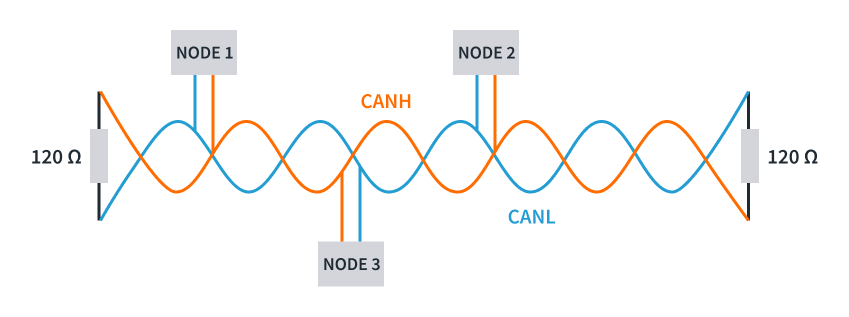
\includegraphics[width=0.8\linewidth]{image/interface-can-bus.png}
    \caption{Hardware Interface of CAN Bus.}
    \label{fig:CAN Bus}
\end{figure}

%============================================================================
% END OF CHAPTER 2
%============================================================================

  \section{METHODOLOGY}

\subsection{Thesis Framework}
\hspace{1.27cm}
The thesis framework presented in \textbf{\autoref{fig:thesis_framework}} outlines the structured methodology adopted for the design, development, and validation of the Delta robot pick-and-place system. The process is divided into three main phases: initial design and component selection, prototype development and software implementation, and system integration, testing, and validation.
\par
\begin{figure}[h]
    \centering
    \includegraphics[page=1, trim=0mm 0mm 0mm 0mm, clip, width=1\linewidth]{image/thesis_framework.png}
    \caption{Thesis Framework.}
    \label{fig:thesis_framework}
\end{figure}
\hspace{1.27cm}
Phase 1 Literature Review and Design: the first phase began with a comprehensive review of existing
Delta robot implementations, analytical kinematic formulations,
vision-based pick-and-place control systems, and relevant
software frameworks including ROS~2 and open-source CAN bus
libraries. Findings from the review directly informed all
subsequent design decisions. The mechanical geometry was
defined by selecting the four kinematic parameters fixed base
triangle side $f$, moving platform triangle side $e$, upper arm
length $r_f$, and forearm length $r_e$ to achieve a
$\pm$150\,mm planar working radius at a nominal pick depth of
$Z = -410$\,mm below the robot base frame. Component selection
covered the RobStride RS-00 quasi-direct-drive actuators, the
Intel RealSense D455 camera, the CAN bus interface hardware,
and the pneumatic solenoid gripper. The complete robot structure,
including the base plate, upper arm brackets, forearm
parallelogram linkages, and moving platform, was modelled in
CAD software prior to fabrication. Structural choices such as
aluminium extrusion profiles for the fixed frame and PLA
3D-printed components for the kinematic links were evaluated
against stiffness, weight, and fabrication cost requirements
at this stage.

\par
\hspace{1.27cm}
Phase 2 Prototype Development and Software
Implementation: the second phase covered mechanical fabrication, assembly, and
the implementation of the complete software stack. The robot
frame was fabricated from aluminium profiles and assembled with
3D-printed PLA joint brackets. Three RobStride RS-00 actuators
were mounted on the base plate and integrated with the host
computer via a USB-to-CAN adapter using the \texttt{python-can}
library operating over the SocketCAN driver. Motor enable,
position command, and encoder feedback routines were implemented
and verified in open-loop tests before the kinematic layer was
added. The ROS~2 software architecture was then constructed as
five coordinated packages: a kinematics node providing
analytical IK and FK solvers, a motion planning node generating
quintic-profiled Cartesian trajectories, a vision pipeline node
integrating HSV blob detection and switchable YOLO11n inference,
a belt prediction node estimating object position at the future
pick instant from measured belt velocity, and a visual
end-effector feedforward correction node that iteratively
reduced the residual camera-to-gripper offset using laser-dot
tracking. Cartesian trajectories are executed using a triangular
velocity profile ($t_{\text{move}} = 2\sqrt{d/a_{\max}}$),
matching the PP-mode trapezoidal planner in each RS-00 motor.
Each package was developed, unit-tested, and
integrated incrementally before system-level testing began.

\par
\hspace{1.27cm}
Phase 3 System Integration, Testing, and
Validation: the third phase brought all hardware and software subsystems
together for end-to-end calibration, tuning, and performance
evaluation. Camera-to-robot frame calibration was performed
using the empirical axis-alignment procedure described in
\autoref{sec:coordinate_transform}, establishing the rotation
matrix $\mathbf{R}$ and translation vector $\mathbf{T}$ of the
hand-eye transform. The analytical IK and FK solvers were
validated at a set of ground-truth positions distributed across
the workspace, with FK position error recorded at each point to
confirm sub-millimetre accuracy. Belt speed was measured by
tracking a fiducial marker across successive camera frames and
computing the pixel displacement per unit time, which was then
converted to physical velocity using the calibrated
pixel-to-mm scale factor. The end-effector correction loop was
tuned by adjusting the feedforward gain and convergence
threshold until the laser dot centroid reached the target pixel
within the required number of correction iterations. Final
end-to-end pick-and-place trials were conducted on the
moving conveyor belt across multiple object positions and
detection conditions. Performance metrics recorded during
these trials included mean and maximum FK position error,
YOLO and HSV detection confidence scores, EE correction
convergence iteration count, pick success rate, and
complete cycle time from object detection to gripper release.
These results are reported and analysed in
Chapter~\ref{ch:results}.
%============================================================================
% MECHANICAL DESIGN SECTION — FULL (matched to CAD drawings)
% Institute of Technology of Cambodia
% Delta Robot Vision-Based Control System
% Academic Year: 2025-2026
%============================================================================

\subsection{Mechanical Design}
\hspace{1.27cm}
The mechanical design of the Delta robot was developed with four
concurrent objectives: achieving sufficient structural rigidity
to maintain kinematic accuracy during dynamic pick-and-place
cycles, minimising the moving mass of the parallel linkage
assembly to preserve the high-acceleration capability inherent
to the Delta architecture, ensuring that all components could
be fabricated or sourced within the constraints of a university
laboratory environment, and keeping total material cost within a
budget appropriate for an educational prototype. The robot frame
combines aluminium extrusion profiles for the stationary base
structure with 3D-printed PLA components for the kinematic
linkages and mounting brackets, and uses carbon fibre tube stock
for the forearm rods where moving inertia is the dominant design
constraint. The finalised kinematic parameters are $f = 157$\,mm,
$e = 35$\,mm, $r_f = 200$\,mm, and $r_e = 400$\,mm, selected to
achieve a $\pm$150\,mm planar working radius at a nominal pick
depth of $Z = -500$\,mm (platform Z) below the robot base frame.

%--------------------------------------------------------------------
\subsubsection{Fixed Base Design}
\hspace{1.27cm}
The fixed base is the stationary platform to which all three
RobStride RS-00 actuators are mounted and from which all
kinematic calculations are referenced. As shown in
\textbf{\autoref{fig:base_design}}, the assembly consists of
three main component types: aluminium extrusion profiles (Item~1)
forming the three sides of the equilateral triangular frame,
carbon fibre support rods (Item~2) used as structural stiffening
members, and 3D-printed PLA corner bracket assemblies (Item~3)
that join the extrusion profiles at the $120^{\circ}$ vertices
and provide the mounting interface for the RobStride RS-00
actuators. The joints are secured with M4 cap-head bolts and
T-nuts inserted into the extrusion channels. The base triangle
has a side length of $f = 157$\,mm.\par
\hspace{1.27cm}
Aluminium extrusion was selected for the primary structural
members because it provides a high stiffness-to-weight ratio,
allows motor mounting positions to be adjusted along the profile
channels during assembly to achieve the correct actuator angular
spacing, and can be cut and drilled with standard workshop
tooling. The entire base assembly is mounted rigidly on a
vertical support structure above the conveyor belt workspace,
establishing the fixed reference coordinate frame for all IK
and FK computations. Any deflection or displacement of the base
under dynamic loading directly corrupts this reference and
degrades absolute positioning accuracy across the workspace.

\begin{figure}[h]
    \centering
    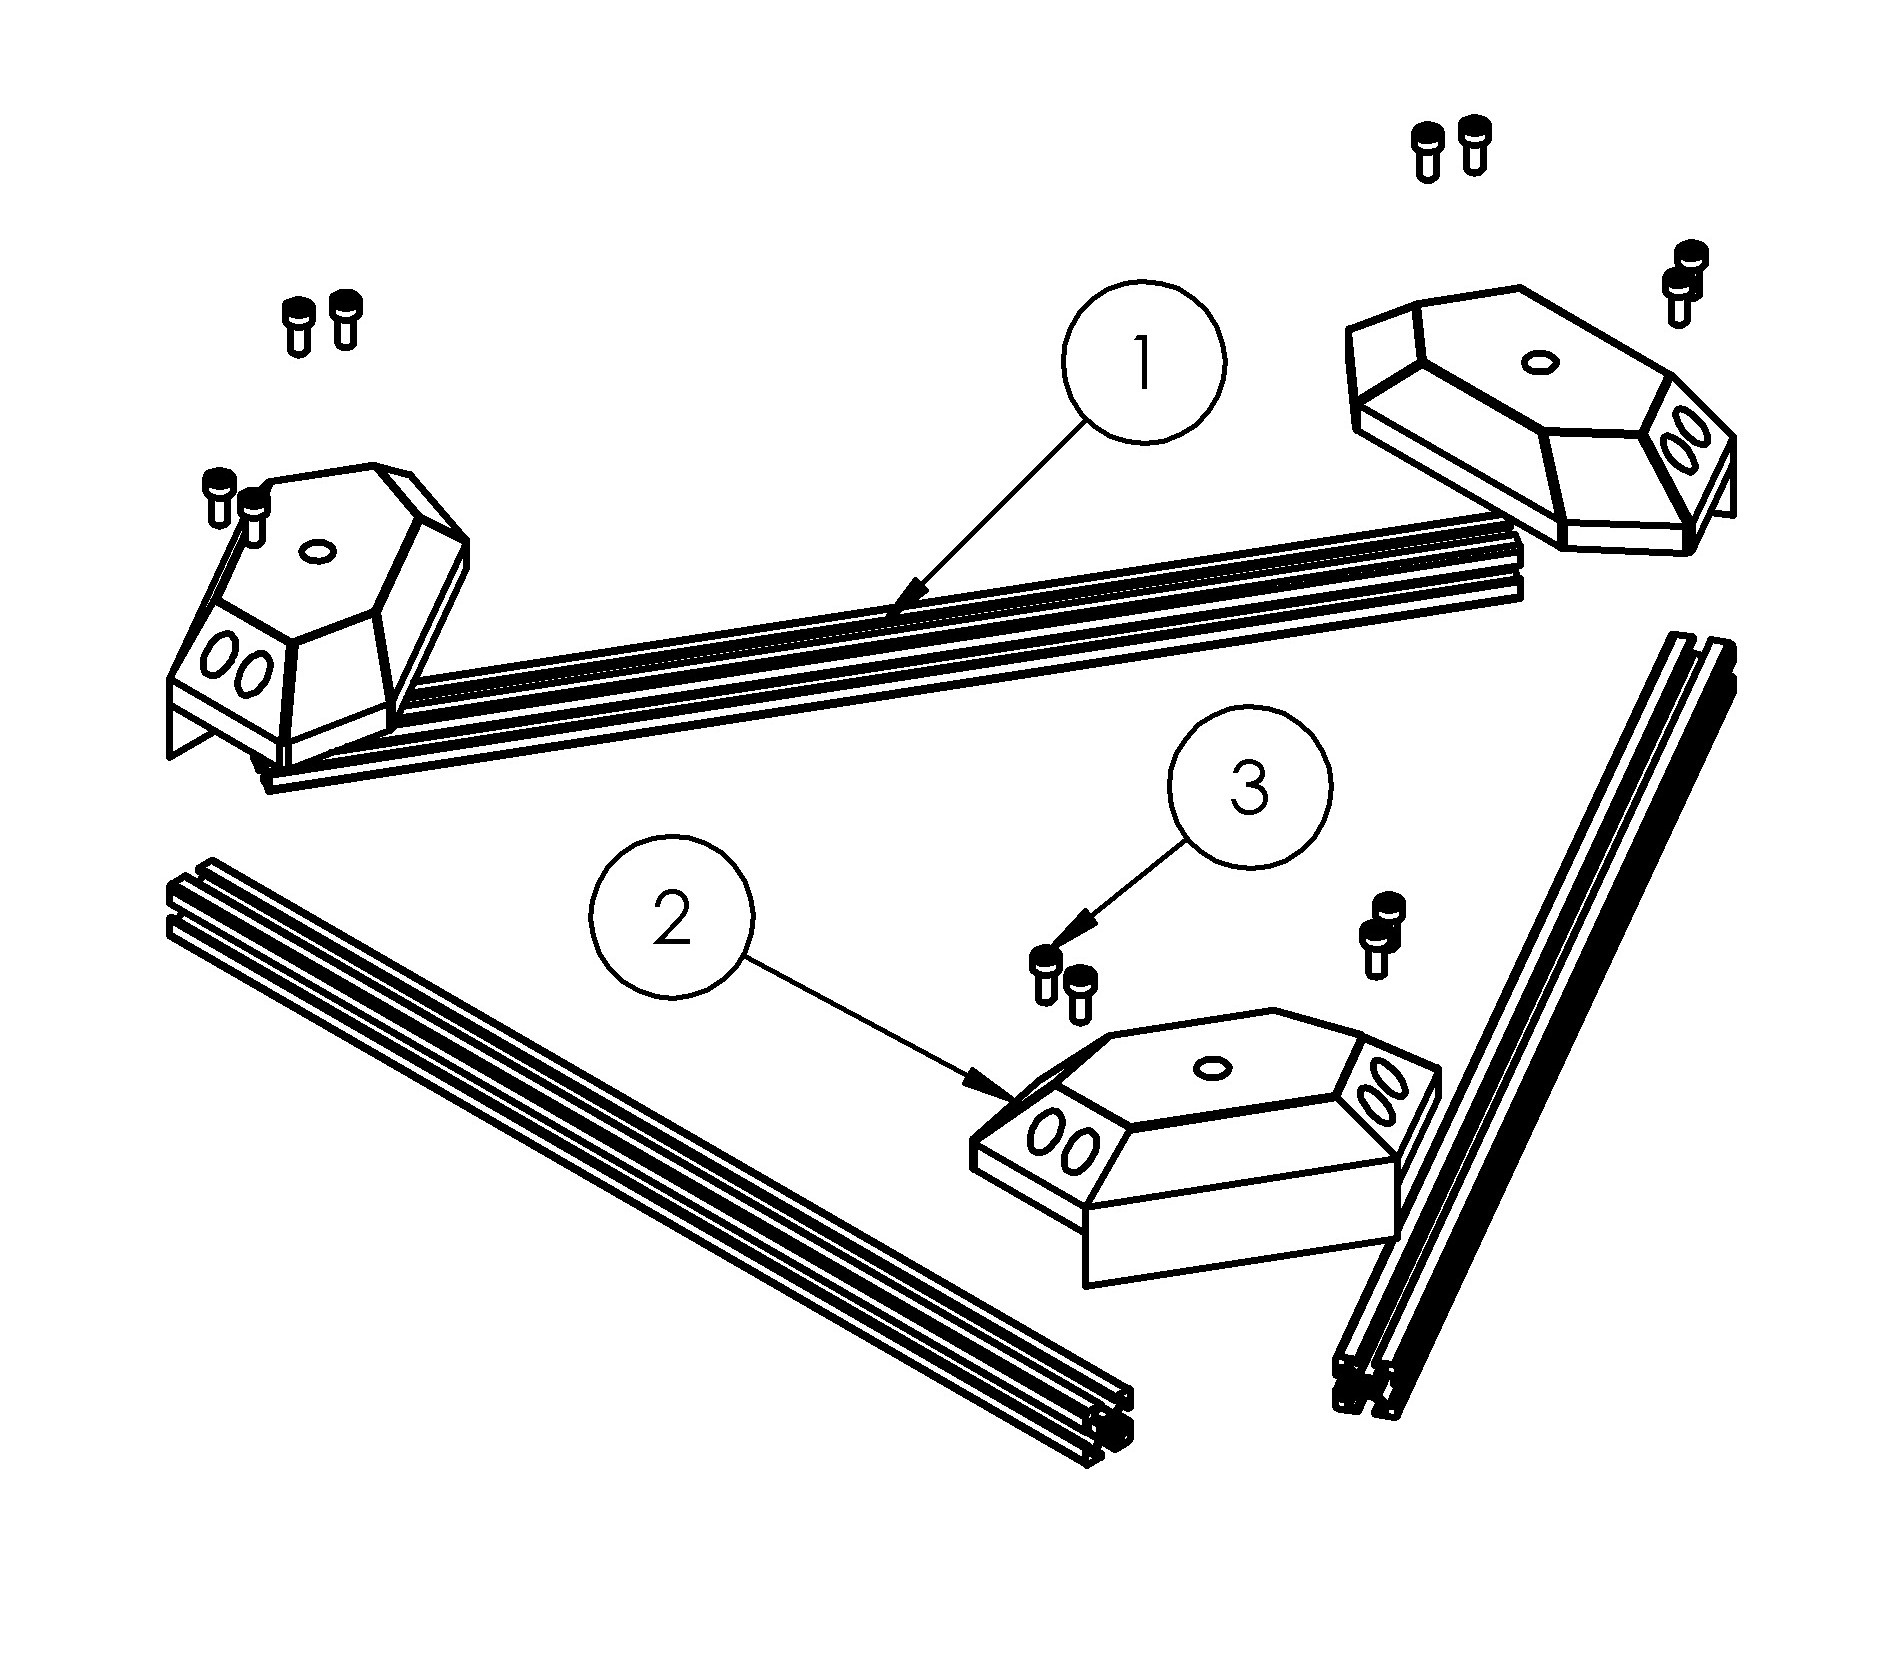
\includegraphics[width=0.70\linewidth]{image/Assem1111.JPG}
    \caption{Base Design of Robot}
    \label{fig:base_design}
\end{figure}

\begin{table}[ht]
    \centering
    \caption{Fixed Base Design Bill of Materials.}
    \label{tab:base_components}
    {\small
    \begin{tabular}{clc}
        \hline
        \textbf{Item} & \textbf{Description} & \textbf{Qty} \\
        \hline
        1 & Aluminium extrusion profile $20 \times 20$\,mm & 3 \\
        2 & 3D-printed PLA corner bracket and motor mount                    & 3 \\
        3 & M4 cap-head bolts and T-nuts  & 12 \\
        \hline
    \end{tabular}}
\end{table}

%--------------------------------------------------------------------
\subsubsection{Bicep Arm Design}
\hspace{1.27cm}
Each upper arm assembly connects one RobStride RS-00 actuator
output shaft to the upper ball-joint end of the corresponding
forearm parallelogram. The exploded view in
\textbf{\autoref{fig:upper_arm}} shows all seven components of
the assembly. The PLA arm body (Item~3) spans $r_f = 200$\,mm
between the motor flange and the forearm joint. On the motor
side, a circular clamping flange (Item~2) with a central
coupling hub (Item~1) is bolted to the arm body using M4
socket-head bolts (Item~5) and secured against the RobStride
RS-00 motor housing via M4 bolts and lock nuts (Item~4). On
the forearm side, the arm terminates in a ball-stud retention
socket that accepts the upper rod-end ball joint of the forearm
parallelogram. The complete assembly is fastened to the motor
output flange using the M4 fastener set (Item~5) distributed
around the bolt circle, with a retaining ring (Item~6) and
the RobStride RS-00 motor body (Item~7, Peak T = 14\,N\,m)
completing the sub-assembly.\par
\hspace{1.27cm}
The PLA arm body was sized to withstand the bending moment
generated by the combined weight and inertia of the forearm
and moving platform during rapid acceleration at the rated
peak torque of 14\,N\,m. The clamping hub ensures a rigid
connection to the motor shaft so that any angular compliance
at this interface, which would manifest as a systematic
position error across the entire workspace, is eliminated.

\begin{figure}[h]
    \centering
    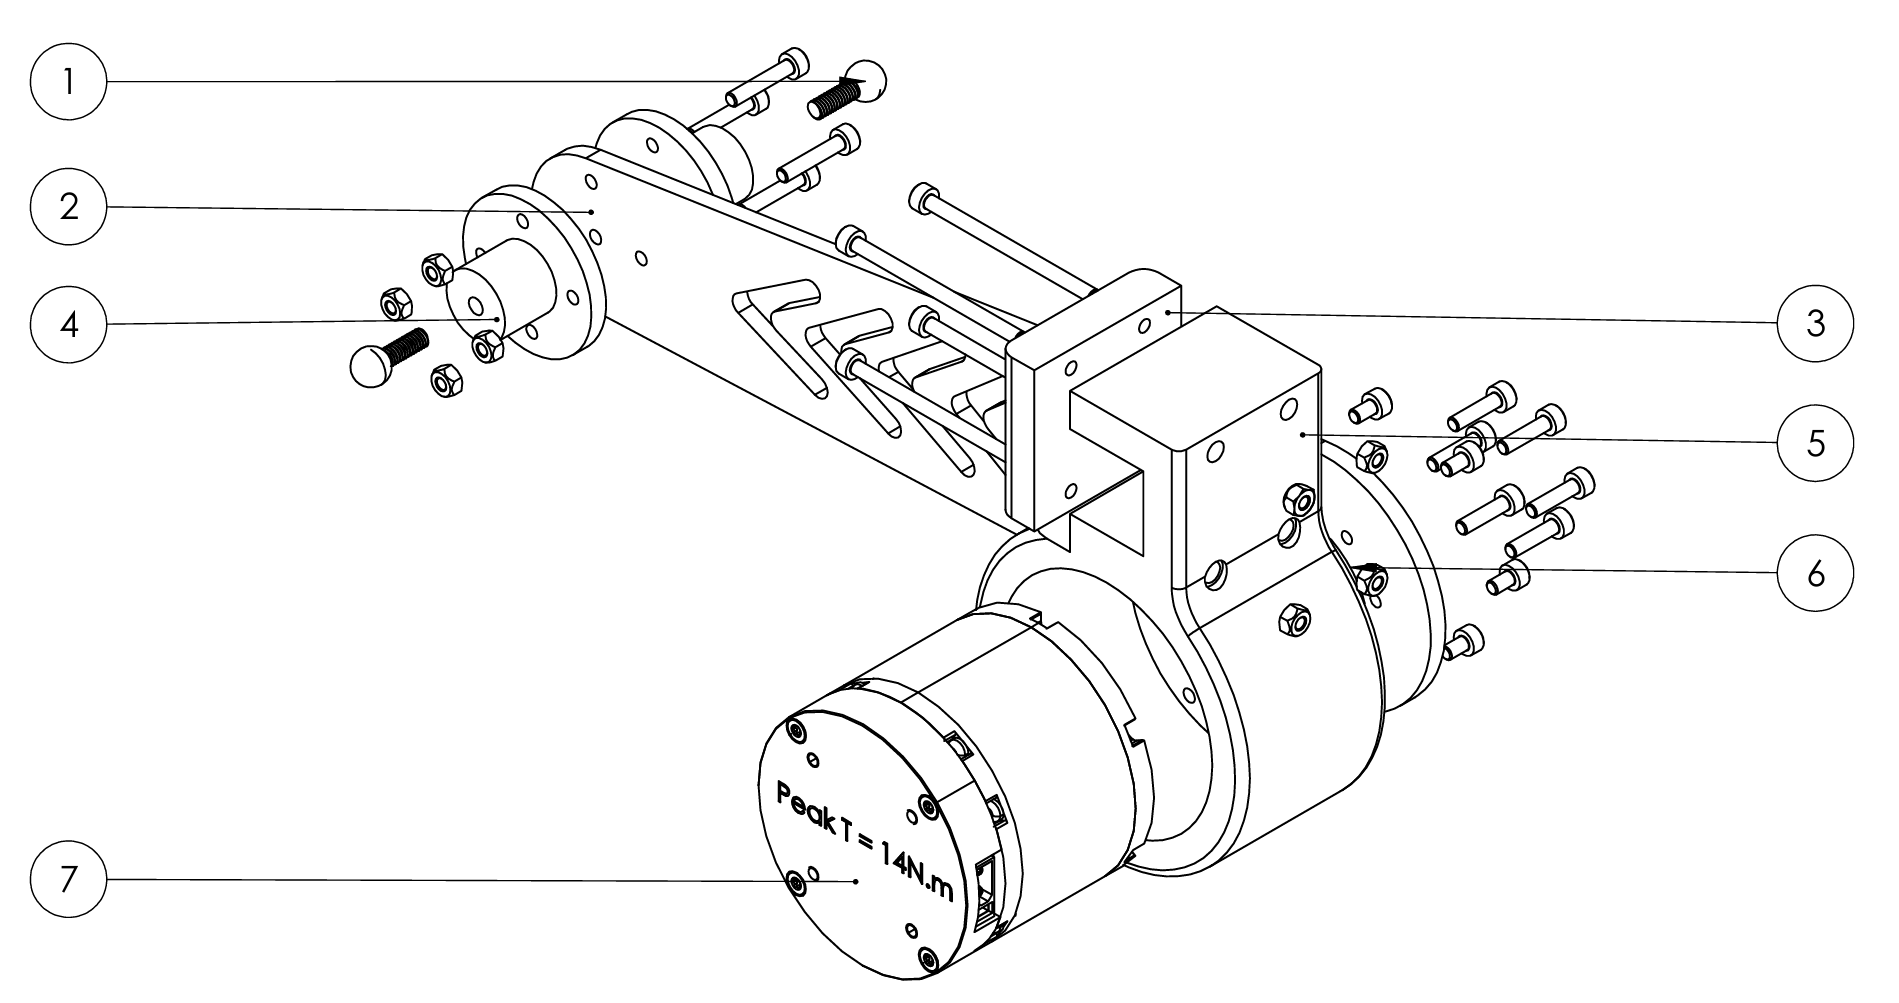
\includegraphics[width=0.85\linewidth]{image/upperarm.png}
    \caption{Bicep Arm of Robot}
    \label{fig:upper_arm}
\end{figure}

\begin{table}[ht]
    \centering
    \caption{Upper Arm Assembly Bill of Materials.}
    \label{tab:upper_arm_components}
    {\small
    \begin{tabular}{clc}
        \hline
        \textbf{Item} & \textbf{Description} & \textbf{Qty} \\
        \hline
        1 & Coupling hub (clamping insert)           & 1 \\
        2 & Circular motor flange plate              & 1 \\
        3 & 3D-printed PLA upper arm body ($r_f = 200$\,mm) & 1 \\
        4 & M4 lock nuts                             & 4 \\
        5 & M4 socket-head cap screws                & 8 \\
        6 & Retaining ring                           & 1 \\
        7 & RobStride RS-00 actuator (Peak T = 14\,N\,m) & 1 \\
        \hline
    \end{tabular}}
\end{table}

%--------------------------------------------------------------------
\subsubsection{Forearm And Moving Platform Design}
\hspace{1.27cm}
The lower arm of each kinematic chain is a parallelogram
linkage connecting the upper arm ball joint to one vertex of
the moving platform. As illustrated in
\textbf{\autoref{fig:lower_arm}}, the assembly consists of
three component types. Item~1 is the carbon fibre forearm rod
of length $r_e = 400$\,mm, terminated at both ends with
aluminium rod-end ball-joint connectors that are press-fitted
and secured with set screws. Two such rods form each
parallelogram pair. Item~2 is the M4 grub screw set used to
lock the rod-end connector to the carbon fibre tube. Item~3 is
the CNC-machined aluminium platform junction plate at the lower
end of the assembly, which provides the bolt pattern for
connecting the forearm ball joints to the moving platform
vertices.\par
\hspace{1.27cm}
The parallelogram geometry is the defining kinematic feature
of the Delta robot: by constraining the two rods to remain
parallel at all configurations, it enforces the condition that
the moving platform undergoes no rotation, maintaining a fixed
end-effector orientation regardless of position within the
workspace \autocite{clavel-1990}. Carbon fibre tube was
selected for the forearm rods because the rods are the only
structural members that undergo full three-dimensional motion
at operating speed. Their mass contributes directly to the
effective inertia seen at the end-effector: reducing rod mass
lowers the torque demand on the actuators during rapid
accelerations and reduces the tendency for the lightweight
parallel linkages to excite structural resonance. The
centre-to-centre spacing between the two rods in each
parallelogram is set equal to the side length $e = 35$\,mm
of the moving platform equilateral triangle, which is the
geometric condition required to maintain the parallelogram
constraint across the full range of joint angles.

\begin{figure}[h]
    \centering
    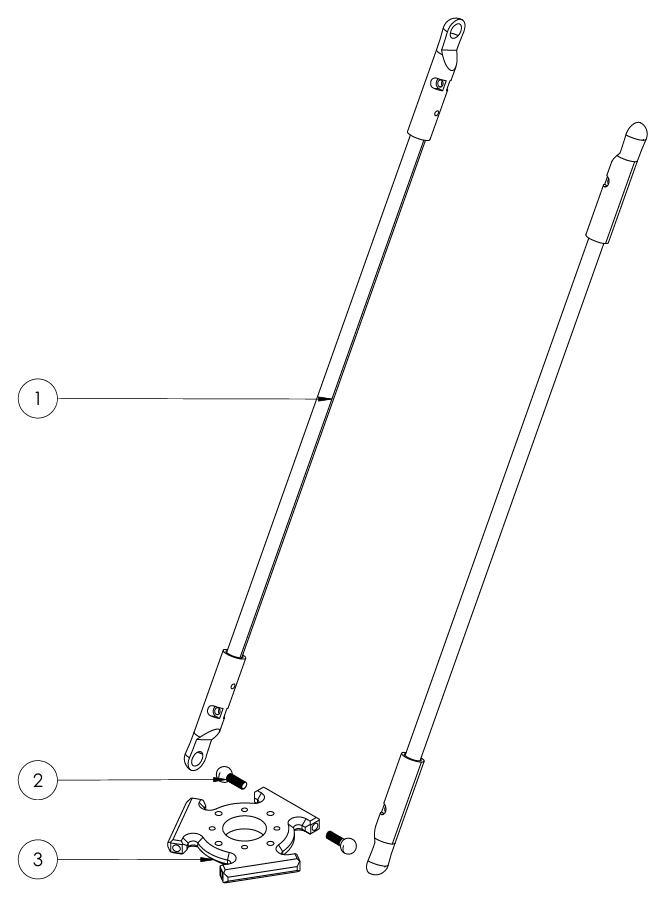
\includegraphics[width=0.55\linewidth]{image/lowerarm.png}
    \caption{Forearm and Moving Plate of Robot}
    \label{fig:lower_arm}
\end{figure}

\begin{table}[ht]
    \centering
    \caption{Lower Arm (Forearm) Assembly Bill of Materials.}
    \label{tab:lower_arm_components}
    {\small
    \begin{tabular}{clc}
        \hline
        \textbf{Item} & \textbf{Description} & \textbf{Qty} \\
        \hline
        1 & Carbon fibre rod with aluminium rod-end
            ball-joint connectors ($r_e = 400$\,mm) & 2 \\
        2 & M4 grub screws (rod-end locking)         & 4 \\
        3 & CNC-machined aluminium platform
            junction plate                           & 1 \\
        \hline
    \end{tabular}}
\end{table}

%--------------------------------------------------------------------
\subsubsection{End-Effector Design}
\hspace{1.27cm}
The end-effector assembly, shown in
\textbf{\autoref{fig:end_effector}}, is a 10-component
sub-assembly mounted below the moving platform. The assembly
integrates a pneumatically actuated two-finger mechanical jaw
gripper, a 650\,nm red-dot laser diode module for end-effector
position tracking, and the structural mounting hardware that
connects the complete assembly to the moving platform centre
boss.\par
\hspace{1.27cm}
Starting from the top of the assembly, Item~1 is the toothed
PLA gripper finger, which has a serrated contact profile to
improve grip on smooth surfaces. Item~2 is the laser diode
module mounting post that positions the 650\,nm beam centrally
between the two jaw fingers and directs it vertically downward
along the end-effector $Z$-axis. Item~3 is the M4 bolt set
used to secure the gripper structure to the cylinder. Item~4
is the M4 finger-to-carrier bolt set fastening the fingers
to the jaw carrier. Item~5 is the CNC-machined aluminium jaw
carrier plate, which transmits the pneumatic cylinder force to
both finger tips simultaneously. Item~6 is the lock-nut set
retaining the assembly. Item~7 is the flat aluminium L-bracket
that mounts the gripper body to the platform junction interface.
Item~8 is the double-acting pneumatic cylinder that actuates
the jaws; pressurised air drives the jaws closed and reversing
the supply opens them. Item~9 is the 3D-printed PLA platform
interface flange that bolts the complete end-effector to the
central boss of the moving platform. Item~10 is the M4 bolt
set securing the flange to the platform.\par
\hspace{1.27cm}
The solenoid valve controlling the pneumatic cylinder is
commanded via CAN ID\,4, with \texttt{004\#01} to close and
\texttt{004\#00} to open. The 5\,mW, 650\,nm laser module
operates continuously during pick-and-place trials and
provides the fiducial dot used by the visual end-effector
feedforward correction loop: the camera detects the laser dot
projected onto the belt surface, computes the pixel offset
between the dot centroid and the target object centroid, and
issues iterative correction commands until alignment converges
before the gripper descends to the pick depth.\par
\hspace{1.27cm}
The vertical distance from the moving platform centre to the
jaw finger contact face defines the end-effector offset
$\delta z$, which is added to the platform $z$-coordinate in
the IK solver when computing the joint angles required to
position the gripper tips at the belt surface. This offset
was measured from the fabricated assembly and is listed in
\autoref{tab:mechanical_params}.

\begin{figure}[h]
    \centering
    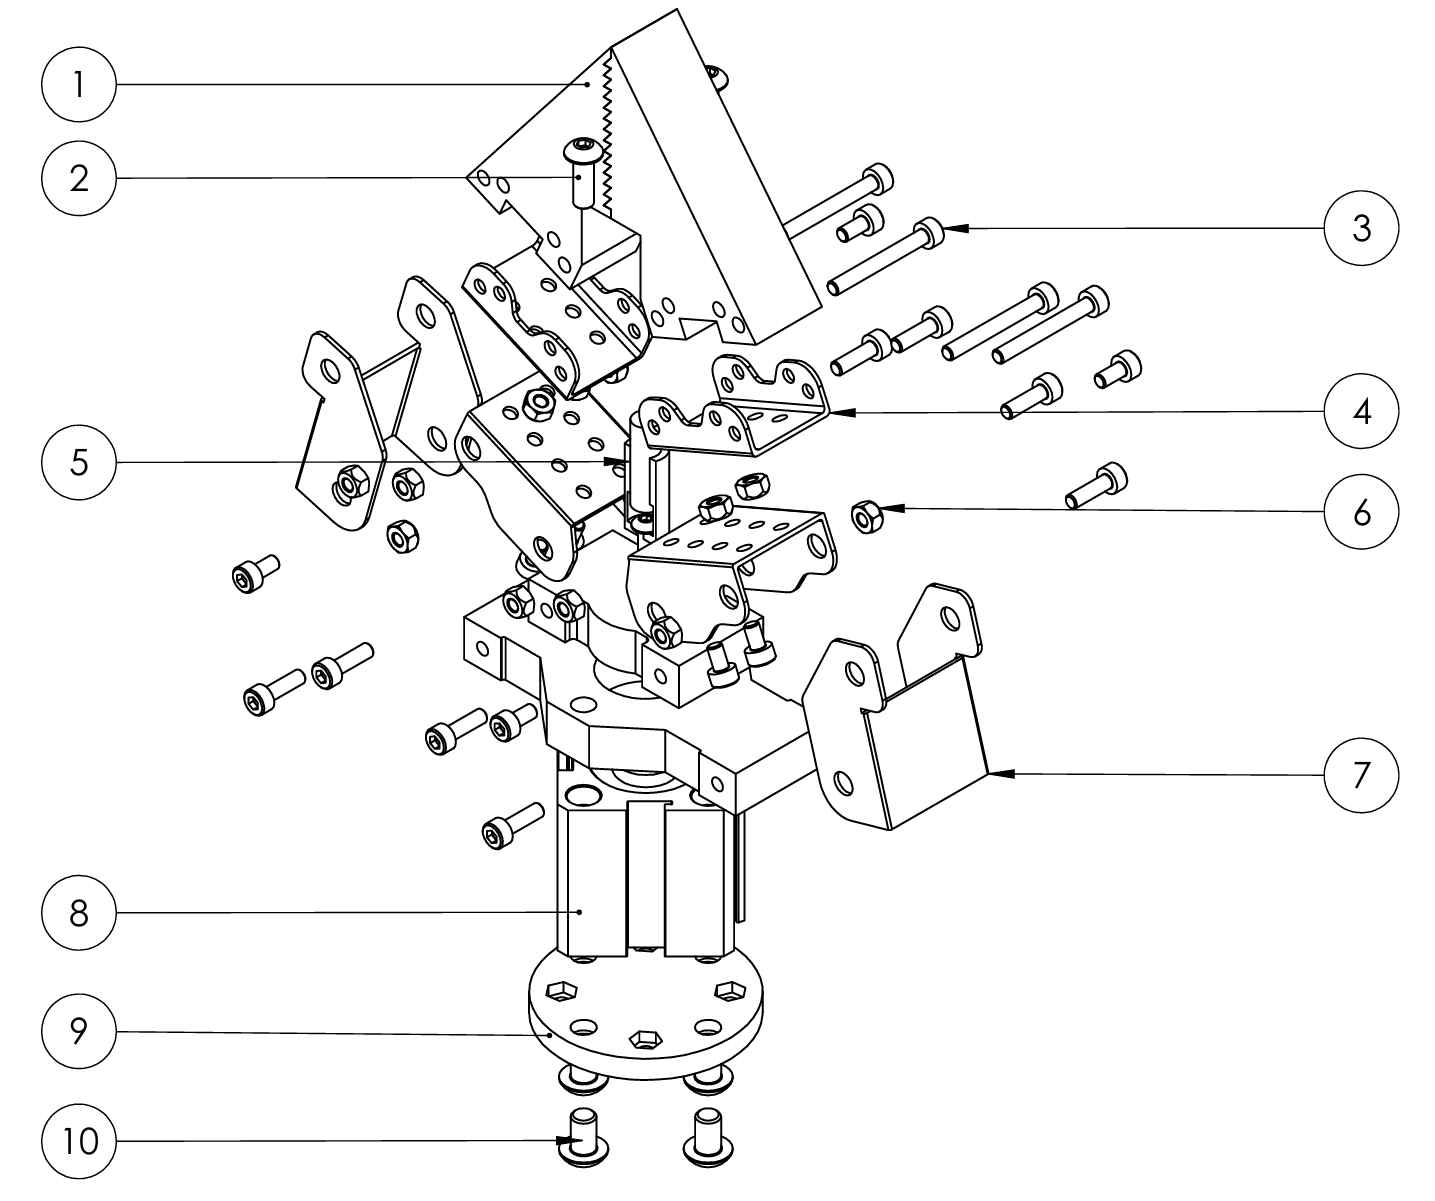
\includegraphics[width=0.75\linewidth]{image/end_effector.png}
    \caption{End-Effector of Robot}
    \label{fig:end_effector}
\end{figure}

\begin{table}[ht]
    \centering
    \caption{End-Effector Assembly Bill of Materials.}
    \label{tab:end_effector_components}
    {\small
    \begin{tabular}{clc}
        \hline
        \textbf{Item} & \textbf{Description} & \textbf{Qty} \\
        \hline
        1  & 3D-printed PLA toothed gripper finger         & 2 \\
        2  & Laser diode module mounting post (650\,nm, 5\,mW)     & 1 \\
        3  & M4 gripper structure-to-cylinder bolt set             & 2 \\
        4  & M4 finger-to-carrier bolt set                         & 4 \\
        5  & CNC aluminium jaw carrier plate                       & 1 \\
        6  & Lock nuts                                             & 12 \\
        7  & Aluminium L-bracket (gripper-to-platform)             & 2 \\
        8  & Double-acting pneumatic cylinder                      & 1 \\
        9  & 3D-printed PLA platform interface flange              & 1 \\
        10 & M4 flange-to-platform bolt set                        & 4 \\
        \hline
    \end{tabular}}
\end{table}

%--------------------------------------------------------------------
\subsubsection{Design Parameters Summary}
\hspace{1.27cm}
The complete mechanical parameters of the fabricated Delta robot
prototype are summarised in \autoref{tab:mechanical_params}.
These values were used directly as inputs to the analytical IK
and FK solvers described in \autoref{sec:kinematics}.

\begin{table}[h]
    \centering
    \caption{Delta Robot Mechanical Design Parameters.}
    \label{tab:mechanical_params}
    \begin{tabular}{llcc}
        \hline
        \textbf{Parameter} & \textbf{Symbol} &
        \textbf{Value} & \textbf{Unit} \\
        \hline
        Base triangle side length   & $f$
            & 157     & mm \\
        Platform triangle side      & $e$
            & 35      & mm \\
        Upper arm length            & $r_f$
            & 200     & mm \\
        Forearm length              & $r_e$
            & 400     & mm \\
        Nominal pick depth (platform) & $Z_{\text{pick}}$
            & $-500$  & mm \\
        Target workspace radius     & $r_w$
            & 150     & mm \\
        End-effector offset         & $\delta z$
            & 150     & mm \\
        Actuator peak torque        & $T_{\text{peak}}$
            & 14      & N\,m \\
        \hline
        Base frame material         & --
            & \multicolumn{2}{c}{Aluminium extrusion
              $20 \times 20$\,mm} \\
        Upper arm material          & --
            & \multicolumn{2}{c}{3D-printed PLA} \\
        Forearm rod material        & --
            & \multicolumn{2}{c}{Carbon fibre tube} \\
        Moving platform material    & --
            & \multicolumn{2}{c}{CNC aluminium} \\
        Gripper body material       & --
            & \multicolumn{2}{c}{CNC aluminium} \\
        Finger material             & --
            & \multicolumn{2}{c}{3D-printed PLA (toothed)} \\
        Gripper actuation           & --
            & \multicolumn{2}{c}{Pneumatic (double-acting)} \\
        EE laser                    & --
            & \multicolumn{2}{c}{650\,nm, 5\,mW red-dot diode} \\
        Gripper CAN ID              & --
            & \multicolumn{2}{c}{ID\,4
              (\texttt{004\#01} / \texttt{004\#00})} \\
        \hline
    \end{tabular}
\end{table}

%============================================================================
% END OF MECHANICAL DESIGN SECTION
%============================================================================

\subsection{Hardware Selection}
\subsubsection{Motors}
\hspace{1.27cm}
The RobStride RS-00 is a compact quasi-direct-drive (QDD)
actuator integrating a brushless DC motor, a low-ratio
planetary gearbox, and an absolute magnetic encoder in a
single module. QDD actuators offer high backdrivability,
low reflected inertia, and high-bandwidth torque control
compared to conventional high-ratio gearbox motors, making
them well suited for compliant robotic manipulation. Three
RS-00 units (CAN IDs 1, 2, and 3) are used, one per
kinematic chain, mounted on the fixed base frame.

\begin{figure}[h]
    \centering
    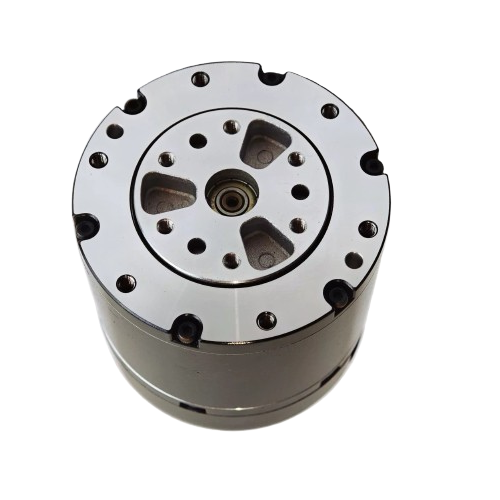
\includegraphics[width=0.4\linewidth]{image/ROBSTRIDE-00.png}
    \caption{RobStride RS-00 quasi-direct-drive actuator.}
    \label{fig:motor}
\end{figure}

\begin{table}[htbp]
    \centering
    \caption{RobStride RS-00 Specifications.}
    \label{tab:motor_spec}
    {\small
    \begin{tabular}{lcc}
        \hline
        \textbf{Parameter} & \textbf{Value} & \textbf{Unit} \\
        \hline
        Rated voltage           & 24      & V \\
        Peak torque             & 14.0    & N\,m \\
        Max motor speed         & 50.0    & rad/s \\
        Max motor acceleration  & 100.0   & rad/s$^2$ \\
        Medium preset velocity  & 25.0    & rad/s \\
        Medium preset accel.    & 50.0    & rad/s$^2$ \\
        Communication           & CAN bus & -- \\
        CAN baudrate            & 1       & Mbit/s \\
        Encoder type            & Absolute magnetic & -- \\
        Control mode            & Position-Profile (PP) & -- \\
        \hline
    \end{tabular}}
\end{table}

\hspace{1.27cm}
In this system the RS-00 is operated exclusively in
\textbf{Position-Profile (PP) mode}, whose internal
control architecture is illustrated in
\textbf{\autoref{fig:pp_mode}}. PP mode executes a
complete closed-loop trajectory internally within the
motor controller. The host PC supplies three set-points
per move: target angle, set speed, and set acceleration.
The onboard \textbf{t-curve planning algorithm} generates
a time-optimal trapezoidal velocity profile from these
set-points and outputs a continuously updated planning
perspective (the instantaneous position reference).\par
\hspace{1.27cm}
The planning perspective is compared with the current
encoder angle to form a position error. This error is
amplified by the proportional gain $K_p$ of the position
loop, whose output becomes the velocity reference. A
second subtraction node compares this reference against
the current speed measured by the encoder to produce a
velocity error, which feeds a \textbf{PI velocity
controller}. The PI output is a torque (current) demand
that passes through a \textbf{torque protection} saturation
block, limiting the command to the rated peak current to
prevent thermal damage.\par
\hspace{1.27cm}
The protected torque demand is decomposed into two current
references following field-oriented control (FOC)
conventions: the quadrature-axis reference
$i_{q,\text{ref}}$ (torque-producing component) is set to
the torque demand value, while the direct-axis reference
$i_{d,\text{ref}} = 0$ (flux component) is held at zero
for maximum torque-per-ampere efficiency. Two independent
\textbf{PI current controllers} regulate $i_q$ and $i_d$
respectively, producing voltage references that are
modulated by a \textbf{Space Vector PWM (SVPWM)} block.
The SVPWM signals drive the \textbf{three-phase voltage
inverter}, which applies the commanded phase voltages to
the brushless DC motor windings to produce the desired
torque and motion.

\begin{figure}[h]
    \centering
    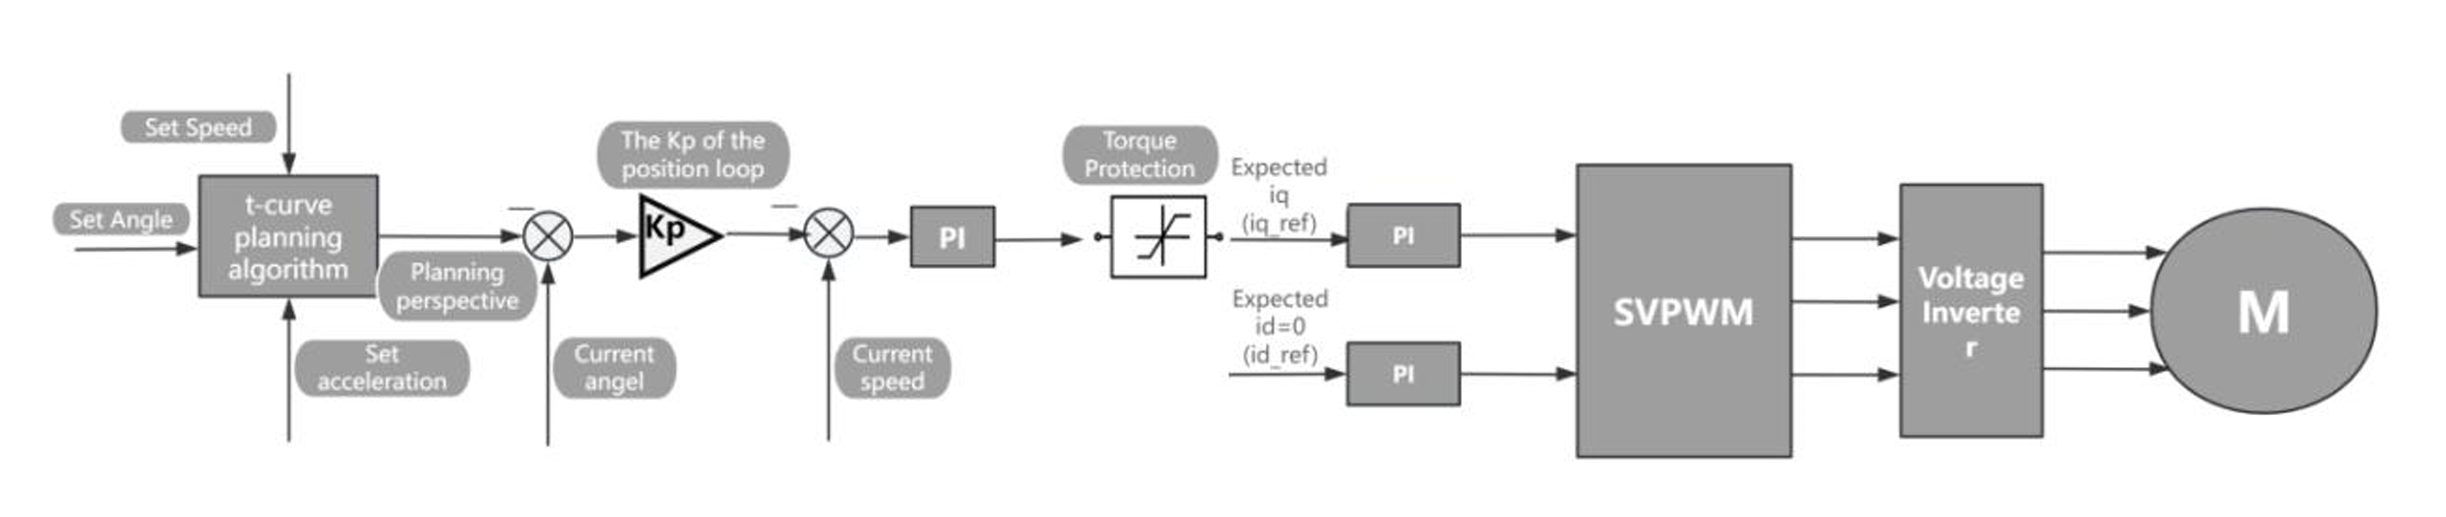
\includegraphics[width=0.95\linewidth]{image/PPmode.png}
    \caption{Position-Profile (PP) Mode Control Architecture
             of The RobStride RS-00 Actuator.}
    \label{fig:pp_mode}
\end{figure}
\subsubsection{Motor Bridge}
\begin{itemize}
    \par
    \hspace{1.27cm}
    The RobStride RS-00 motors are driven directly over a CAN bus at 1\,Mbit/s using a USB-to-CAN adapter connected to the host PC running Ubuntu 22.04 with ROS\,2 Humble. The SocketCAN Linux kernel driver exposes the CAN interface as a standard network interface (\texttt{can0}), enabling direct read/write access from Python via the \texttt{python-can} library. The three motor driver boards are connected in a daisy-chain topology on the same CAN bus, with termination resistors at both ends.
    \par
    \begin{figure}[h]
        \centering
         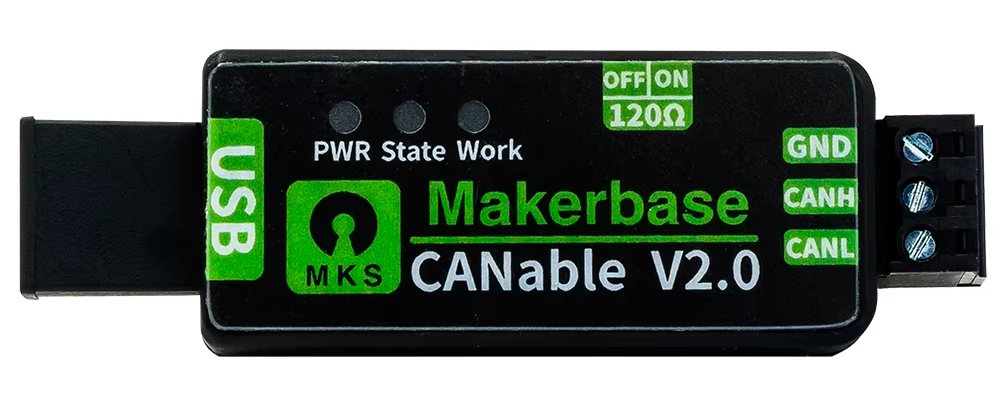
\includegraphics[width=0.4\linewidth]{image/can driver.png}
        \caption{USB-to-CAN Adapter for ROS\,2 CAN Bus Interface.}
        \label{fig:driver}
    \end{figure}
    \begin{table}[htbp]
        \centering
        \caption{CAN Bus Interface Specifications.}
        {\small
        \begin{tabular}{lcc}
            \textbf{Parameter} & \textbf{Specification} & \textbf{Unit} \\
            \hline
            Interface type    & USB-to-CAN      & — \\
            Linux driver      & SocketCAN       & — \\
            Baudrate          & 1               & Mbit/s \\
            Topology          & Daisy-chain     & — \\
            Motor nodes       & 3 (IDs 1, 2, 3) & — \\
            Gripper node      & 1 (ID 4)        & — \\
            Host OS           & Ubuntu 22.04    & — \\
            \ChangeRT{1.5pt}
        \end{tabular}}
        \label{tab:driver_spec}
    \end{table}
\end{itemize}
\subsubsection{Pneumatic Solenoid Valve}
\hspace{1.27cm}
The pneumatic solenoid valve used in this system is a
five-port, two-position (5/2) single-solenoid directional
control valve, as shown in \textbf{\autoref{fig:pneumatic_valve}}.
The valve body is constructed from anodised aluminium alloy
with an IP65-rated solenoid coil housing, rated for continuous
duty (100\,\% ED) at DC\,24\,V, drawing 200\,mA at a power
consumption of 4.8\,W. The operating voltage range is
DC\,20.4\,V to 28.4\,V, making it directly compatible with
the 24\,V power rail of the system.

\par
\hspace{1.27cm}
The valve has three external connections visible in
\textbf{\autoref{fig:pneumatic_valve}}: a single \textbf{Air
Inlet Hole} on the underside that receives compressed air from
the air container, and two \textbf{Air Outlet Holes} (port~A
and port~B) on the upper face that route air to the two
chambers of the double-acting pneumatic cylinder on the
gripper assembly. When the solenoid coil is de-energised, the
internal spring returns the spool to its default position,
directing compressed air from the inlet to outlet port~A and
venting port~B to atmosphere, which drives the gripper jaws to
the open position. When the solenoid coil is energised by the
CAN ID\,4 command \texttt{004\#01}, the magnetic force shifts
the spool to connect the inlet to port~B and vent port~A,
driving the jaws to the closed (grip) position. Sending
\texttt{004\#00} de-energises the coil and returns the valve
to the open state.\par
\hspace{1.27cm}
The 5/2 configuration was selected because the double-acting
pneumatic cylinder on the end-effector requires independent
pressurisation of both its extend and retract chambers to
produce positive gripping force in both the closing and
opening directions, rather than relying on a return spring.
This provides faster jaw opening response and more consistent
release behaviour than a spring-return cylinder, which is
important for repeatable object placement at the drop position
during pick-and-place cycles. The IP65 ingress protection
rating ensures reliable operation in the laboratory environment
where compressed air fittings may introduce moisture.

\begin{figure}[h]
    \centering
    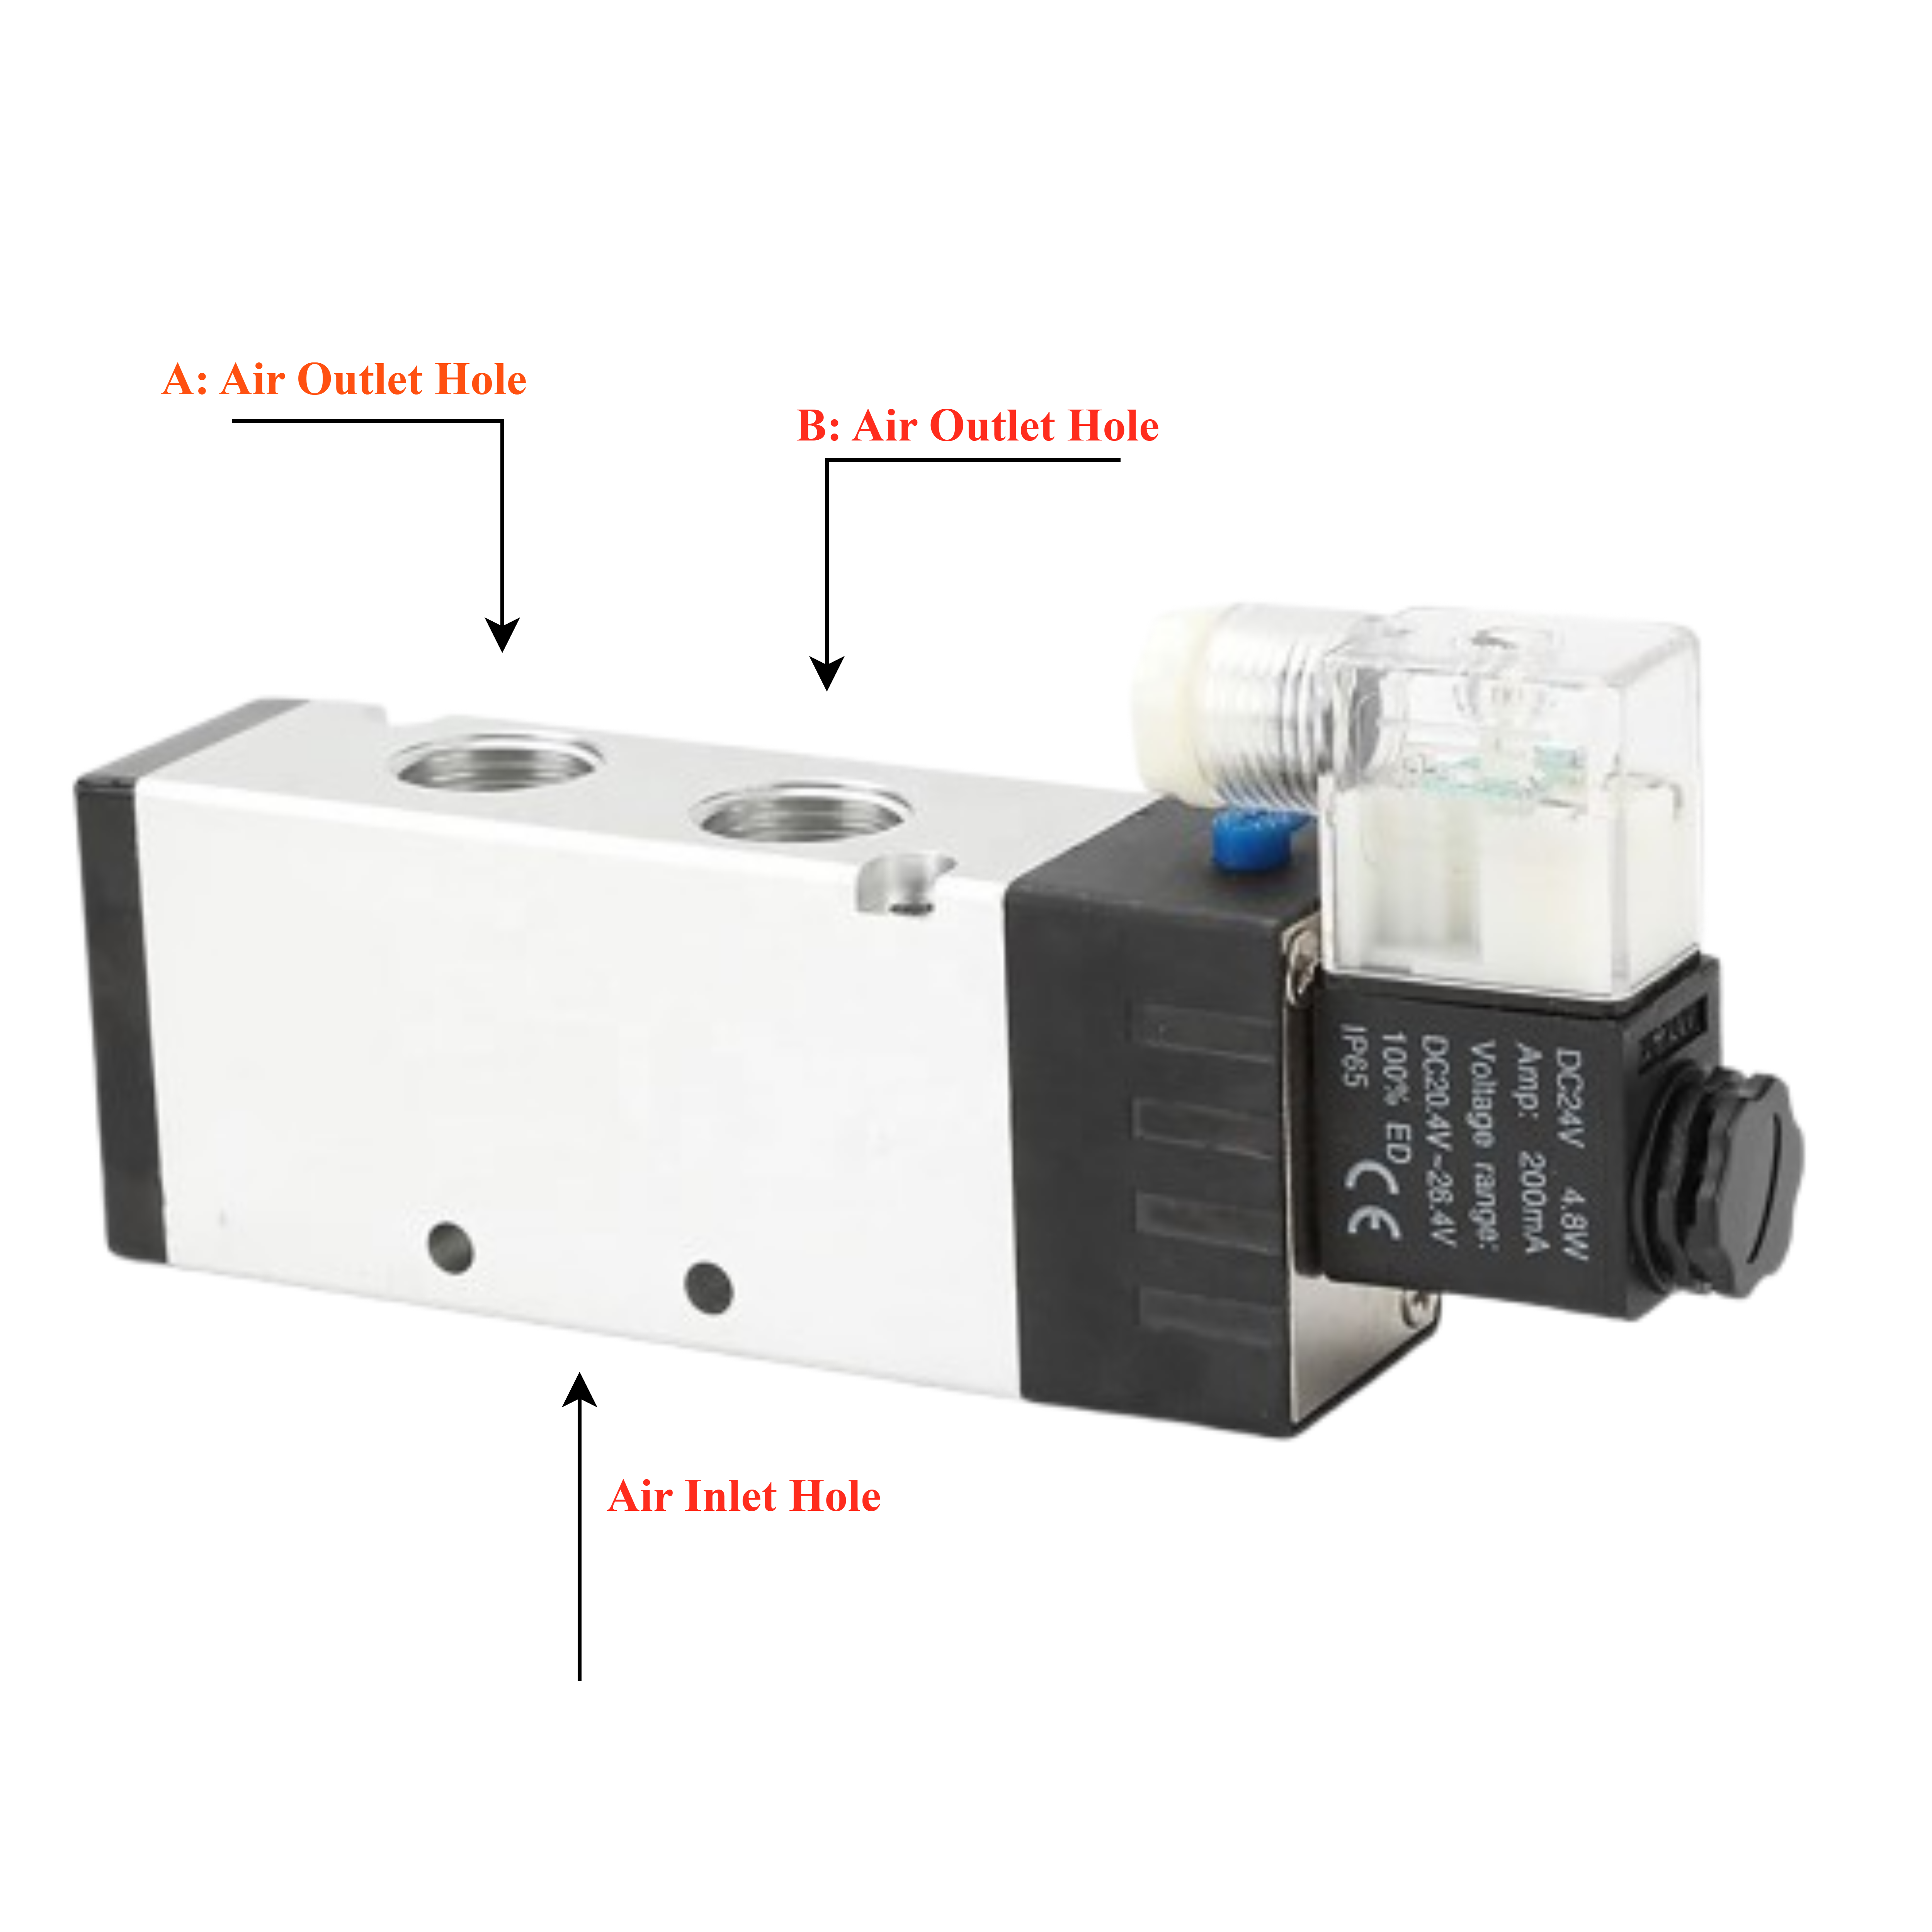
\includegraphics[width=0.60\linewidth]{image/Pneumatic.png}
    \caption{5/2 single-solenoid directional control valve
             (DC\,24\,V, 4.8\,W, 200\,mA, IP65) showing the
             air inlet hole on the underside and the two air
             outlet holes (port~A and port~B) on the upper
             face that supply the double-acting gripper
             cylinder.}
    \label{fig:pneumatic_valve}
\end{figure}

\begin{table}[htbp]
    \centering
    \caption{Pneumatic Solenoid Valve Specifications.}
    \label{tab:pneumatic_spec}
    {\small
    \begin{tabular}{lcc}
        \hline
        \textbf{Parameter} & \textbf{Value} & \textbf{Unit} \\
        \hline
        Valve type              & 5/2 single-solenoid & -- \\
        Solenoid voltage        & DC 24       & V \\
        Voltage range           & DC 20.4--28.4 & V \\
        Power consumption       & 4.8         & W \\
        Solenoid current        & 200         & mA \\
        Duty cycle              & 100 (continuous) & \% ED \\
        Ingress protection      & IP65        & -- \\
        Air inlet               & 1 port (underside) & -- \\
        Air outlets             & 2 ports A, B (top) & -- \\
        Control interface       & CAN ID\,4   & -- \\
        Close command           & \texttt{004\#01} & -- \\
        Open command            & \texttt{004\#00} & -- \\
        \hline
    \end{tabular}}
\end{table} 
\subsubsection{Camera and Vision Hardware}
\hspace{1.27cm}
The Intel RealSense D455 is a stereo-capable RGB-D camera selected for this system due to its wide field of view, stable USB\,3.0 interface, and well-supported ROS\,2 driver. In this application, only the RGB stream is used for object detection and localisation. Since all pick targets lie on the conveyor belt surface at a fixed and known elevation of $Z = -410$\,mm below the robot base frame, per-pixel depth sensing is not required. Object positions are recovered from 2D pixel coordinates using the known camera intrinsics and the fixed belt depth, as described in the vision pipeline section. The camera connects to the host PC via USB\,3.0 and is driven by the \texttt{librealsense2} driver and \texttt{realsense2\_camera} ROS\,2 wrapper node.

\par
    \begin{figure}[h]
        \centering
         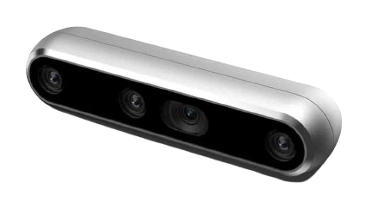
\includegraphics[width=0.4\linewidth]{image/Realsense D455.png}
        \caption{The Intel RealSense D455.}
        \label{fig:Realsense D455}
    \end{figure}

\begin{table}[htbp]
    \centering
    \caption{Intel RealSense D455 Specifications.}
    {\small
    \begin{tabular}{lcc}
        \textbf{Parameter} & \textbf{Specification} & \textbf{Unit} \\
        \hline
        Depth technology     & Active IR stereo   & — \\
        Stereo baseline      & 95                 & mm \\
        RGB resolution       & $640 \times 480$   & px \\
        Depth resolution     & $848 \times 480$   & px \\
        Frame rate           & 30                 & fps \\
        Depth range          & 0.4 -- 6.0         & m \\
        RGB FOV (H$\times$V) & 87$\times$58       & deg \\
        Interface            & USB 3.0            & — \\
        \ChangeRT{1.5pt}
    \end{tabular}}
    \label{tab:camera_spec}
\end{table}

\subsubsection{Output2CAN}
\hspace{1.27cm}
The Output2CAN board is a custom CAN-based controller developed by the Cambodia Team and used in many projects specifically to control pneumatic actuators. In the Delta robot system, this board is responsible for managing the vacuum gripper through solenoid valve control. At its core, the board is powered by an STM32F103C8T6 microcontroller, which receives CAN messages from the main controller and triggers digital outputs accordingly. These outputs are connected to N-MOSFET drivers capable of switching standard 12V solenoid valves on and off. Four output channels are available (D1–D4). Communication with the robot’s CAN network is handled via an onboard TJA1050 transceiver, which ensures robust and noise-resistant signaling. The board features clearly labeled JST connectors for each output, simplifying cable management and allowing for quick installation and maintenance. Power is supplied via separate VCC and GND lines, while the logic section is powered by a regulated 3.3V supply.\par
\begin{figure}[h]
    \centering  
    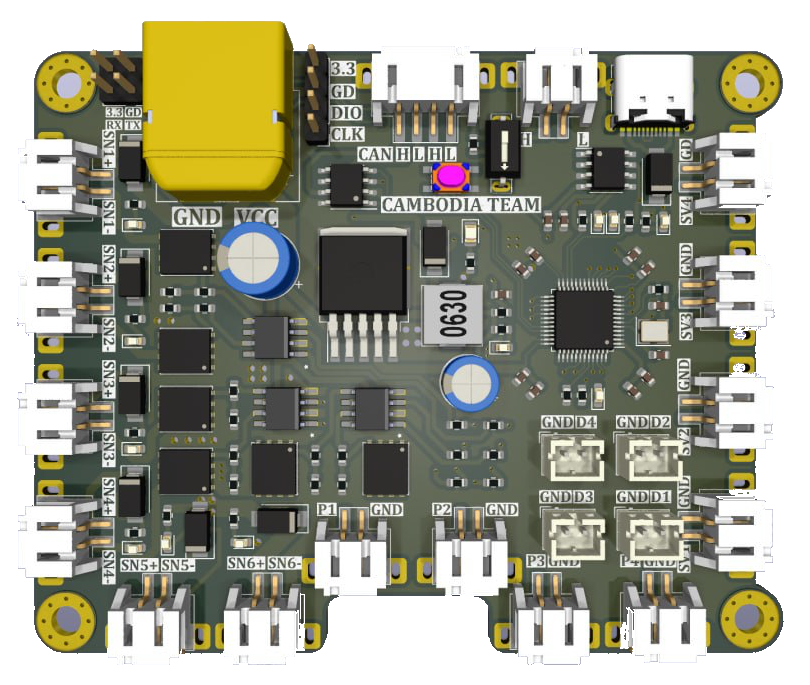
\includegraphics[width=0.5\linewidth]{image/output2can.png}
    \caption{Output2CAN board.}
    \label{fig:output2can}
\end{figure}
\hspace{1.27cm}
By delegating pneumatic control to this dedicated module, the overall wiring complexity is reduced and the system becomes more modular and maintainable. This makes the Output2CAN board an efficient solution for decentralized pneumatic actuation within the Delta robot platform.

\subsubsection{Conveyor Belt Hardware}
\hspace{1.27cm}
The conveyor belt is driven by a NEMA-17 stepper motor through a 1:36 planetary gearbox, with a timing pulley of circumference 153.9\,mm ($\pi \times 49$\,mm). The stepper motor is controlled by an Arduino microcontroller running at 1/8 microstepping (1600 steps/revolution) with a step pulse delay of 104\,\textmu s, yielding a physically measured belt speed of 12.85\,mm/s in the $Y$ direction (toward the EXIT side of the workspace).
\par
    \begin{figure}[h]
        \centering
         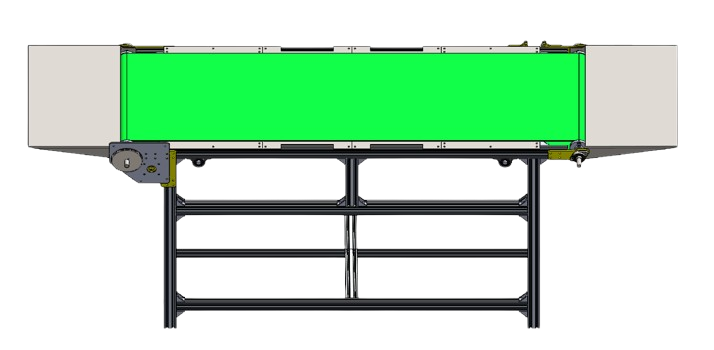
\includegraphics[width=0.7\linewidth]{image/Conveyer.png}
        \caption{Conveyer Belt.}
        \label{fig:Conveyer}
    \end{figure}

%============================================================================
\subsection{Kinematic Model Development}
\hspace{1.27cm}
The kinematic model of the Delta robot establishes the mathematical relationship between joint space (motor angles $\theta_1, \theta_2, \theta_3$) and Cartesian task space (end-effector position $x, y, z$). Both forward and inverse kinematics are derived based on the geometric parameters of the robot following the formulation of \autocite{clavel-1990} as implemented by \autocite{mzavatsky-2009}.

\subsubsection{Geometric Parameters}
\hspace{1.27cm}
The Delta robot is characterised by four geometric parameters listed in \textbf{\autoref{tab:delta_params}}. The fixed base equilateral triangle has a side
length of $f = 157$ mm, and the moving platform equilateral triangle has a side
length of $e = 35$ mm. The upper arm length is $r_f = 200$ mm, and the lower arm
(forearm) length is $r_e = 400$ mm. The reference coordinate frame is placed at
the center of symmetry of the fixed base triangle, with the $z$-axis pointing
downward such that all reachable end-effector positions carry negative
$z$-coordinates. \par
\begin{table}[htbp]
    \centering
    \caption{Delta Robot Geometric Parameters.}
    {\small
    \begin{tabular}{clcc}
        \textbf{Symbol} & \textbf{Description} & \textbf{Value} & \textbf{Unit} \\
        \hline
        $f$   & Side length of fixed base triangle   & 157 & mm \\
        $e$   & Side length of moving platform        & 35  & mm \\
        $r_f$ & Upper arm length                      & 200 & mm \\
        $r_e$ & Lower arm (forearm) length             & 400 & mm \\
        \ChangeRT{1.5pt}
    \end{tabular}}
    \label{tab:delta_params}
\end{table}
To simplify the kinematic equations, the effective radius difference is defined as:
\begin{equation}
    \Delta r = \frac{f}{2\sqrt{3}} - \frac{e}{2\sqrt{3}}
             = \frac{157}{2\sqrt{3}} - \frac{35}{2\sqrt{3}}
             \approx 45.34 - 10.10
             = 35.24 \text{ mm}
    \label{eq:delta_r}
\end{equation}
This quantity $\Delta r$ represents the horizontal offset between the base joint
pivot and the effective platform attachment point for each arm, and appears
directly in the inverse kinematics equations.
\par
\begin{figure}[h]
    \centering
    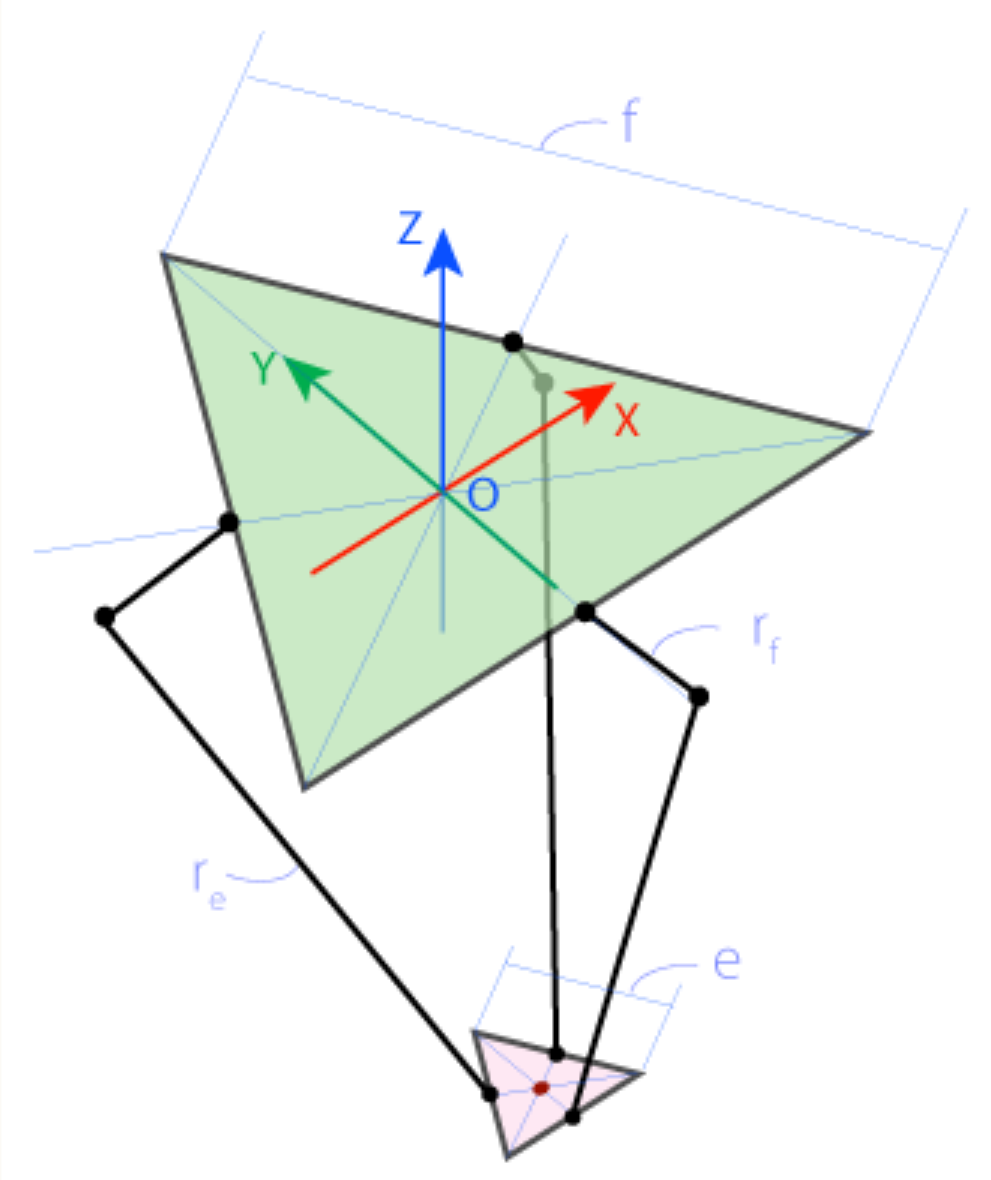
\includegraphics[width=0.6\linewidth]{image/Schem Kinematic.png}
    \caption{Delta Robot Kinematic Scheme ($f=157$\,mm, $e=35$\,mm, $r_f=200$\,mm, $r_e=400$\,mm).}
    \label{fig:kinematic_scheme}
\end{figure}

\subsubsection{Inverse Kinematics}
\hspace{1.27cm}
The inverse kinematics (IK) determines the three joint angles $(\theta_1, \theta_2, \theta_3)$
required to position the end-effector at a desired Cartesian coordinate $(x_0, y_0, z_0)$.
Due to the three-fold rotational symmetry of the Delta robot, each arm is solved independently
after rotating the target coordinates by $0°$, $120°$, and $240°$ respectively about the $z$-axis.

\par\noindent\textbf{Step 1: Coordinate Rotation}\par
\hspace{1.27cm}
For arm $i$ ($i = 1, 2, 3$), the end-effector target point is first rotated into the reference
plane of that arm. Defining the rotation angle $\varphi_i = (i - 1) \times 120°$, the rotated
coordinates are:

\begin{equation}
    x'_i = x_0 \cos\varphi_i + y_0 \sin\varphi_i
    \label{eq:rot_x}
\end{equation}
\begin{equation}
    y'_i = -x_0 \sin\varphi_i + y_0 \cos\varphi_i
    \label{eq:rot_y}
\end{equation}
\begin{equation}
    z'_i = z_0
    \label{eq:rot_z}
\end{equation}

This rotation reduces the 3D problem for each arm to an equivalent planar problem
in the $YZ$ plane of that arm's reference frame.

\par\noindent\textbf{Step 2: Effective Target Point}\par
\hspace{1.27cm}
The effective target point for each arm accounts for the geometric offset $\Delta r$
between the base pivot and the platform joint:

\begin{equation}
    y_{i,\text{eff}} = y'_i - \Delta r = y'_i - 35.24 \text{ mm}
    \label{eq:eff_target}
\end{equation}
\hspace{1.27cm}
The joint angle $\theta_i$ for arm $i$ is then found by solving the intersection of two
circles in the $YZ$ plane: a circle of radius $r_f = 200$ mm centred at the base pivot
$F_i$, and a circle of radius $r_e = 400$ mm centred at the effective target point.

\par\noindent\textbf{Step 3: Planar Circle Intersection}\par
\hspace{1.27cm}
Expanding the two circle equations and subtracting to eliminate the quadratic terms
yields a linear expression. Substituting back gives the following quadratic in $y_J$:
\begin{equation}
    a \cdot y_J^2 + b \cdot y_J + c = 0
    \label{eq:quadratic}
\end{equation}

where:

\begin{equation}
    a = 1 + \left(\frac{z'_i}{y_{i,\text{eff}}}\right)^2
    \label{eq:coeff_a}
\end{equation}

\begin{equation}
    b = \frac{-2 \, y_{i,\text{eff}} \left(r_e^2 - r_f^2 - y_{i,\text{eff}}^2 - z_i^{\prime 2}\right)}
            {2\, y_{i,\text{eff}}^2 + 2\, z_i^{\prime 2}}
    \label{eq:coeff_b}
\end{equation}

\begin{equation}
    c = \left(\frac{r_e^2 - r_f^2 - y_{i,\text{eff}}^2 - z_i^{\prime 2}}
                   {2\, y_{i,\text{eff}}}\right)^2 - r_f^2
    \label{eq:coeff_c}
\end{equation}
\hspace{1.27cm}
The discriminant $D = b^2 - 4ac$ must be non-negative for a valid solution. A negative
discriminant indicates that the target position lies outside the reachable workspace, and
the IK solver immediately rejects the command and returns an error flag before any motor
command is issued.

\par\noindent\textbf{Step 4: Joint Angle Recovery}\par
\hspace{1.27cm}
Selecting the physically meaningful root (the intersection with the smaller $y$-coordinate,
corresponding to the elbow-down configuration):

\begin{equation}
    \theta_i = \text{atan2}\!\left(-z'_i,\ y_J - y_{F_i}\right)
    \label{eq:joint_angle}
\end{equation}
\hspace{1.27cm}
where $y_{F_i}$ is the $y$-coordinate of the base pivot $F_i$. The result is bounded to
the mechanical joint limit $[-10°,\ 90°]$. If the computed angle falls outside this range,
the target is declared unreachable and rejected.\par


\subsubsection{Forward Kinematics}
\hspace{1.27cm}
The forward kinematics (FK) determines the Cartesian end-effector position
$(x_0, y_0, z_0)$ given the three measured joint angles $(\theta_1, \theta_2, \theta_3)$.
In this thesis, FK is not used for primary motion generation but serves as a post-motion
validation step: after each pick-and-place movement, the encoder-read joint angles are
passed through the FK solver and the resulting position is compared against the commanded
target to detect mechanical faults or excessive positional error.

\par\noindent\textbf{Step 1: Upper Arm Tip Positions}\par
\hspace{1.27cm}
For each arm $i$, the Cartesian position of the upper arm tip $J_i$ is computed from
the joint angle $\theta_i$ and the geometric parameters:
\begin{align}
    J_{i,x} &= \left(r_f \cos\theta_i + \Delta r\right)\cos\varphi_i \notag \\
    J_{i,y} &= \left(r_f \cos\theta_i + \Delta r\right)\sin\varphi_i \notag \\
    J_{i,z} &= -r_f \sin\theta_i
    \label{eq:arm_tip}
\end{align}

where $\varphi_i = (i - 1) \times 120°$ is the angular offset of arm $i$ about the $z$-axis.

\par\noindent\textbf{Step 2: Sphere Intersection}\par
\hspace{1.27cm}
The end-effector position lies at the intersection of three spheres, each of radius
$r_e = 400$ mm centred at $J_i$:
\begin{equation}
    \left(x_0 - J_{i,x}\right)^2 +
    \left(y_0 - J_{i,y}\right)^2 +
    \left(z_0 - J_{i,z}\right)^2 = r_e^2,
    \qquad i = 1,\, 2,\, 3
    \label{eq:spheres}
\end{equation}

\par\noindent\textbf{Step 3: Linearisation}\par
\hspace{1.27cm}
Subtracting the equation for $i = 1$ from those for $i = 2$ and $i = 3$ eliminates
the quadratic terms, yielding two linear equations of the form:
\begin{equation}
    x_0 = a_1 z_0 + b_1, \qquad y_0 = a_2 z_0 + b_2
    \label{eq:linear}
\end{equation}
\hspace{1.27cm}
where the constants $a_1$, $a_2$, $b_1$, $b_2$ are derived from the upper arm tip
coordinates $J_i$.

\par\noindent\textbf{Step 4: Quadratic in $z_0$}\par
\hspace{1.27cm}
Substituting Equation~\ref{eq:linear} into the sphere equation for $i = 1$ yields
a scalar quadratic in $z_0$:
\begin{multline}
    \left(a_1^2 + a_2^2 + 1\right) z_0^2
    + 2\Bigl[a_1\!\left(b_1 - J_{1,x}\right)
             + a_2\!\left(b_2 - J_{1,y}\right)
             - J_{1,z}\Bigr]\, z_0 \\
    + \Bigl[\left(b_1 - J_{1,x}\right)^2
            + \left(b_2 - J_{1,y}\right)^2
            + J_{1,z}^2
            - r_e^2\Bigr] = 0
    \label{eq:quadratic_z}
\end{multline}
\hspace{1.27cm}
The physically meaningful solution is the more negative real root, corresponding to
the end-effector position below the base plane. A negative discriminant indicates an
invalid joint configuration. Once $z_0$ is found, $x_0$ and $y_0$ are recovered
directly from Equation~\ref{eq:linear}.

\subsubsection{Workspace Analysis}
\hspace{1.27cm}
The reachable workspace of the Delta robot is the set of all
Cartesian positions $(X, Y, Z)$ for which the analytical IK
solver returns a valid solution with all three joint angles
satisfying $\theta_i \geq 0^{\circ}$. The workspace boundary
was mapped numerically in MATLAB by evaluating the IK solution
over a dense three-dimensional grid of candidate positions and
retaining only those points for which all three limbs yielded
a geometrically feasible configuration. The resulting point
cloud, colour-coded by depth ($Z$ value), is shown in the
side view (XZ plane) in \textbf{\autoref{fig:workspace}}.
The overall shape approximates a flattened hemisphere,
characteristic of the Delta robot geometry defined by the
parameters $f = 157$\,mm, $e = 35$\,mm, $r_f = 200$\,mm,
and $r_e = 400$\,mm \autocite{stock-2003}.
\begin{figure}[h]
    \centering
    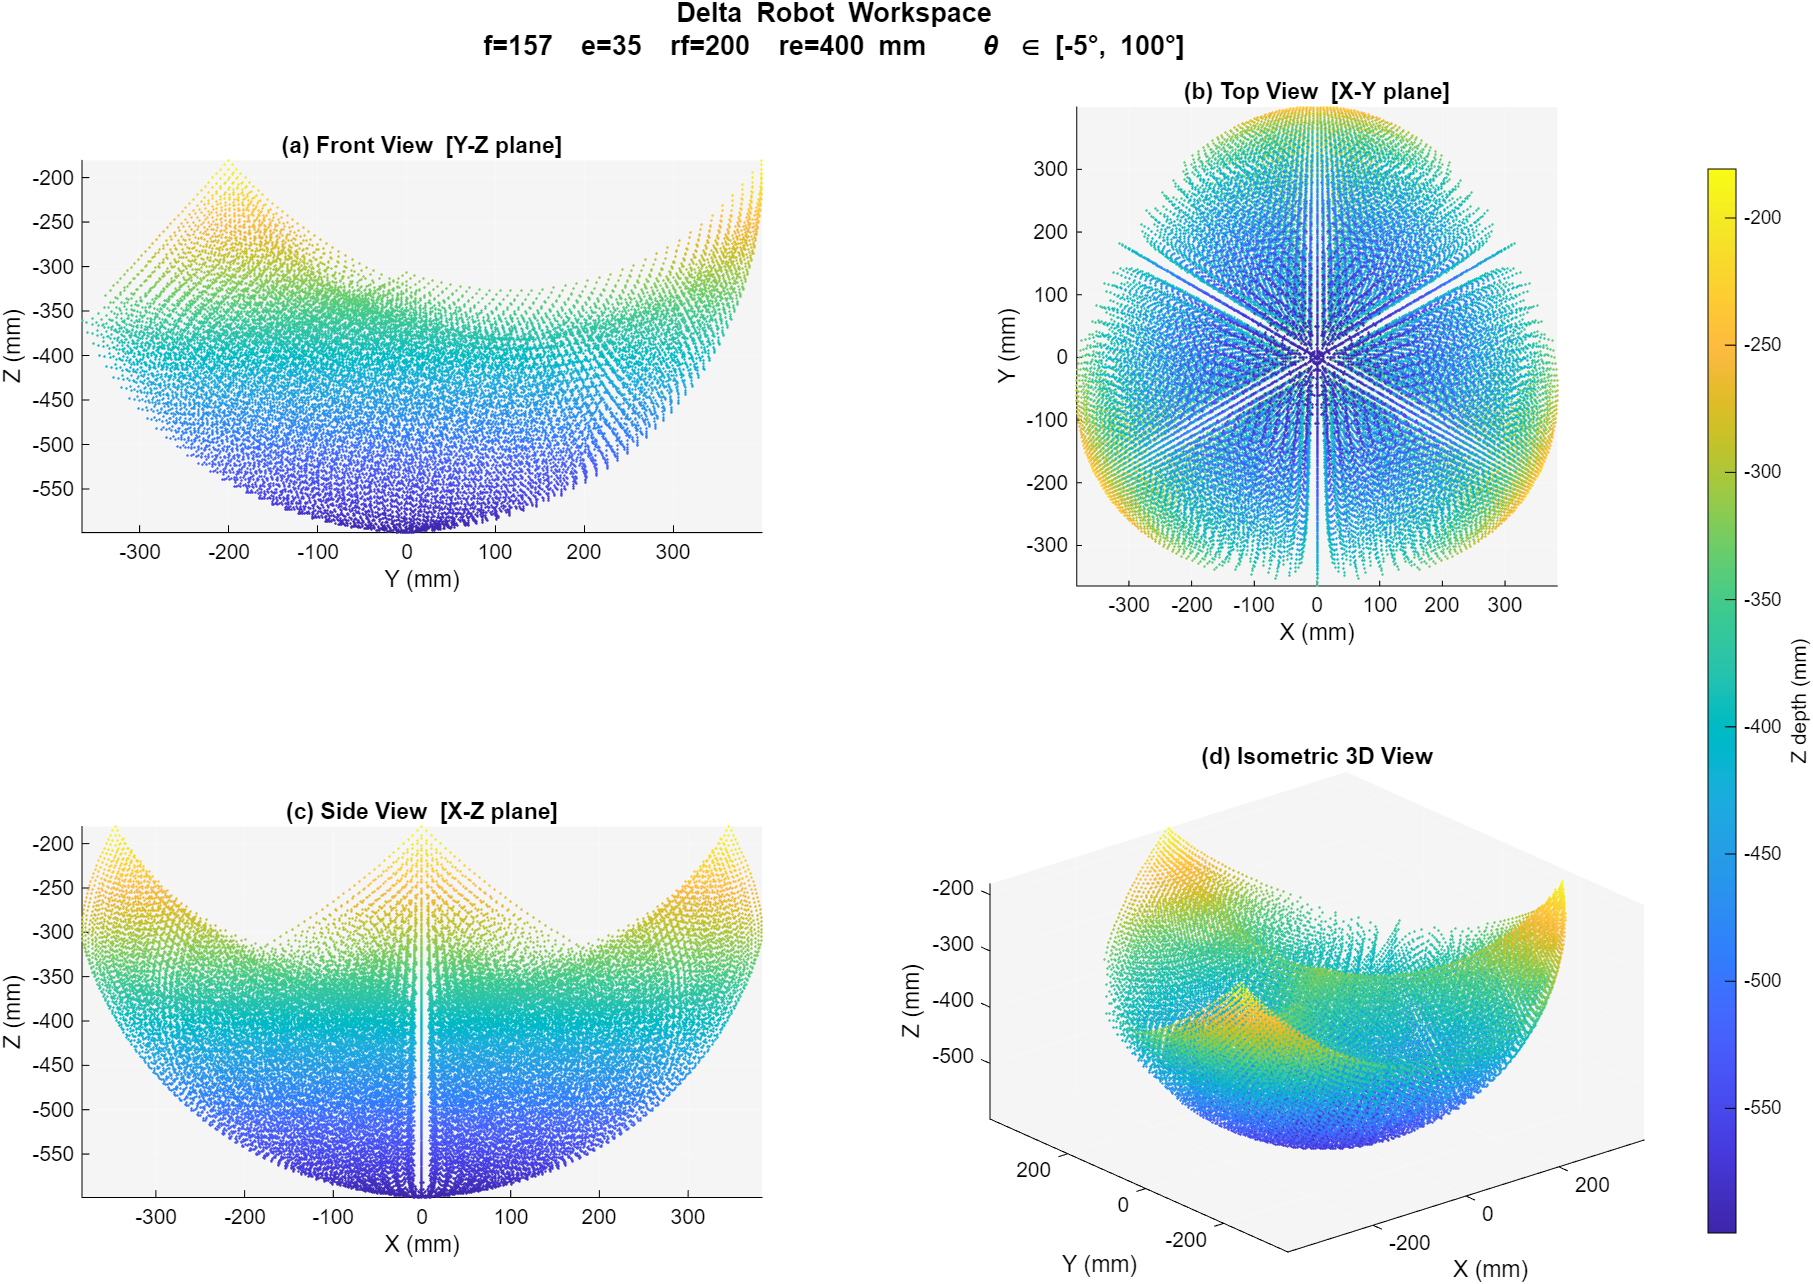
\includegraphics[width=0.9\linewidth]{image/Delta Robot Workspace.png}
    \caption{Full reachable workspace of the Delta robot
             visualised as a 3D point cloud in MATLAB,
             colour-coded by depth $Z$ from the base frame.}
    \label{fig:workspace}
\end{figure}
\par
\hspace{1.27cm}
The full reachable workspace extends considerably beyond the
region that is practically usable for pick-and-place
operations. The upper portions of the workspace (small
negative $Z$ values, yellow-green region in
\textbf{\autoref{fig:actual_workspace}}) correspond to
configurations where the upper arms approach horizontal,
which reduces the effective torque output of the actuators
and brings the forearm parallelograms close to a singular
configuration. The lower boundary is determined by the
maximum extension of the forearms at full vertical reach.
To avoid these mechanical extremes and to constrain the
robot to a region where positioning accuracy and structural
stiffness are reliably maintained, an operational workspace
sub-region was defined as a rectangular box within the
reachable volume, shown by the black rectangle in
\textbf{\autoref{fig:actual_workspace}}.

\begin{figure}[h]
    \centering
    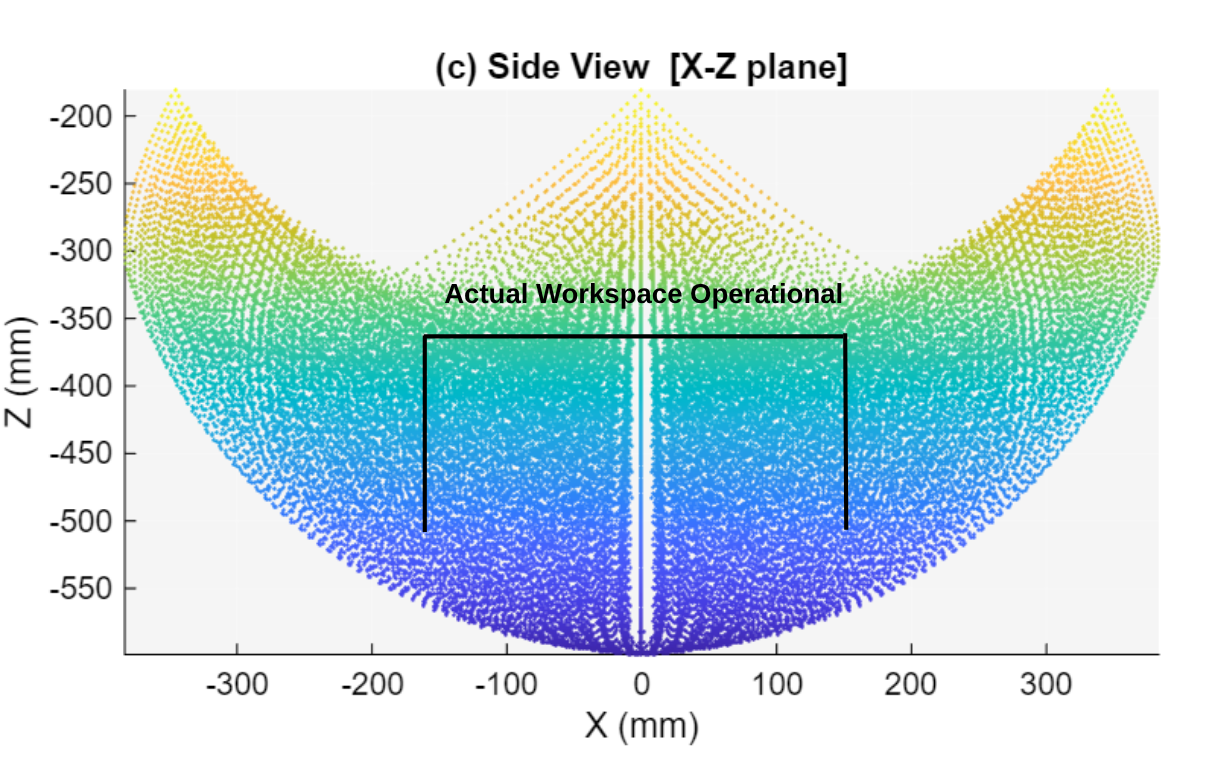
\includegraphics[width=0.7\linewidth]
        {image/Actual worksapce operational.png}
    \caption{Side view (XZ plane) of the full reachable
             workspace with the actual operational workspace
             sub-region indicated by the black rectangle.
             The operational region spans
             $X \in [-150,\, +150]$\,mm and
             $Z \in [-350,\, -500]$\,mm.}
    \label{fig:actual_workspace}
\end{figure}

\par
\hspace{1.27cm}
The physical extent of the operational workspace relative to
the robot structure is shown in
\textbf{\autoref{fig:real_workspace}}. The base frame is
located at the top of the structure, establishing $Z = 0$.
The home position of the end-effector is set at
$(0,\, 0,\, -350)$\,mm, which places the gripper
approximately 350\,mm below the base and serves as the
safe retract position between pick cycles. The conveyor
belt surface lies within the operational depth range of
$Z = -500$\,mm to $Z = -650$\,mm, and the pick-and-place
operations are performed within the horizontal bounds of
$X, Y \in [-150,\, +150]$\,mm. The total vertical travel
from home to the deepest pick position is 300\,mm, and
the total physical height of the robot structure including
the support frame is approximately 650\,mm as annotated in
\textbf{\autoref{fig:real_workspace}}.

\begin{figure}[h]
    \centering
    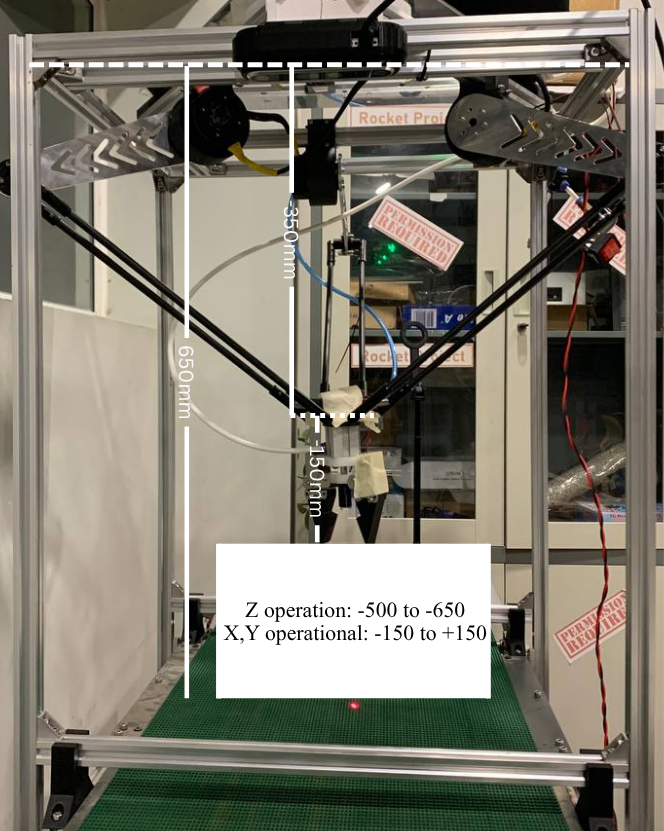
\includegraphics[width=0.525\linewidth]
        {image/real Robot actual operate.png}
    \caption{Physical Delta robot installation showing the
             operational workspace dimensions annotated on
             the real system. The home position is at
             $Z = -350$\,mm below the base frame, and the
             pick depth operates between
             $Z = -500$\,mm and $Z = -650$\,mm. The
             horizontal operational range is
             $X, Y \in [-150,\, +150]$\,mm.}
    \label{fig:real_workspace}
\end{figure}


\par
\hspace{1.27cm}
The operational workspace bounds are enforced in the ROS~2
controller node as hard software limits. Any target
coordinate received from the vision pipeline that falls
outside these bounds is immediately rejected before the
IK solver is invoked, preventing the robot from attempting
to reach a position where accuracy or mechanical safety
cannot be guaranteed. The complete set of software-enforced
workspace parameters is listed in
\textbf{\autoref{tab:workspace}}.
\begin{table}[ht]
    \centering
    \caption{Robot Operational Workspace Parameters.}
    \label{tab:workspace}
    {\small
    \begin{tabular}{lcc}
        \hline
        \textbf{Parameter} & \textbf{Symbol} &
        \textbf{Value} \\
        \hline
        Planar X operational limit  & $X\_LIMIT$
            & $\pm150$\,mm \\
        Planar Y operational limit  & $Y\_LIMIT$
            & $\pm150$\,mm \\
        IK upper ceiling            & $Z\_MAX$
            & $-323$\,mm \\
        Maximum pick depth          & $Z\_MIN$
            & $-560$\,mm \\
        Home position               & $(X_0,Y_0,Z_0)$
            & $(0,\;0,\;-350)$\,mm \\
        Total vertical travel       & $\Delta Z$
            & $210$\,mm \\
        Robot structure height      & $Z\_Belt$
            & $-650$\,mm \\
        \hline
    \end{tabular}}
\end{table}
%============================================================================
%============================================================================
% CONTROL SYSTEM IMPLEMENTATION + VISION PIPELINE
% Institute of Technology of Cambodia
% Delta Robot Vision-Based Control System
% Academic Year: 2025-2026
%============================================================================

\subsection{Control System Implementation}

\subsubsection{System Wiring and Hardware Architecture}
\hspace{1.27cm}
The complete electrical and communication architecture of the
Delta robot system is illustrated in
\textbf{\autoref{fig:wiring_diagram}}. The system is powered
from a 220\,V AC mains supply and is organised into three
distinct subsystems: the Delta robot actuator and CAN bus
subsystem, the conveyor belt drive subsystem, and the
pneumatic gripper subsystem. The host PC running Ubuntu
22.04 and ROS~2 Humble serves as the central computing unit
coordinating all subsystems.

\par
\noindent\textbf{Power Distribution.}\par
\hspace{1.27cm}
A 24\,V regulated DC power supply converts the 220\,V AC
mains input and provides the primary power rail for the
three RobStride RS-00 motor drivers (rated 24\,V). A separate
5\,V rail from the same supply powers the Arduino UNO used for
conveyor belt control. A 24\,V lithium battery pack powers
the DCLAB Smart Driver board that provides the fourth
actuator channel. All power lines are shown as red traces
in \textbf{\autoref{fig:wiring_diagram}}.

\par
\noindent\textbf{CAN Bus Subsystem (Delta Robot Motors).}\par
\hspace{1.27cm}
The three RobStride RS-00 actuators (Motor ID\,1, ID\,2,
and ID\,3) are connected in a daisy-chain CAN bus topology
via CAN\,H and CAN\,L differential signal lines. Each motor
unit integrates a gear stage, the brushless motor body, and
a magnetic encoder within a single compact package. The CAN
bus is interfaced to the host PC through a Makerbase
CANable~V2.0 USB-to-CAN adapter operating on the
\texttt{can0} interface at 1\,Mbit/s. The three motor nodes
drive the three upper arm links (Upper Arm Link~1, 2, and 3)
of the Delta robot respectively. An additional motor is
connected to the DCLAB Smart Driver board via a separate
24\,V power path.

\par
\noindent\textbf{Conveyor Belt Subsystem.}\par
\hspace{1.27cm}
The conveyor belt is driven by a NEMA stepper motor
controlled by a dedicated stepper driver. The stepper driver
receives step and direction pulse signals from an Arduino
UNO, which is powered at 5\,V from the 24\,V supply
auxiliary output. The Arduino UNO communicates with the host
PC via USB serial, allowing the ROS~2 belt prediction node
to read encoder pulses and compute belt velocity. The
complete drive chain from stepper motor through gear and
coil stages to the physical conveyor belt mechanism is
shown in the upper portion of
\textbf{\autoref{fig:wiring_diagram}}.

\par
\noindent\textbf{Pneumatic Gripper Subsystem.}\par
\hspace{1.27cm}
The pneumatic actuation chain begins at an air compressor
that pressurises a portable air container (cylinder).
Compressed air from the container feeds a solenoid valve,
which is controlled by an ON/OFF switch (SW1) signal from
the DCLAB Smart Driver board. When the solenoid is
energised, compressed air is routed to the two-finger
mechanical jaw gripper mounted on the Delta robot
end-effector. The solenoid valve is commanded via the
CAN bus using CAN ID\,4, with command
\texttt{004\#01} to close and \texttt{004\#00} to open,
as described in \autoref{tab:end_effector_components}.

\par
\noindent\textbf{Sensor Interface.}\par
\hspace{1.27cm}
The Intel RealSense D455 camera is connected to the host
PC via a dedicated USB Type-C port. The camera streams RGB
frames and camera intrinsic data directly to the ROS~2
detection node running on the PC. No additional power
supply is required as the camera is bus-powered via USB.

\par
\noindent\textbf{ROS~2 Software Stack.}\par
\hspace{1.27cm}
The ROS~2 software architecture is organised into five
custom packages running on the host PC:
\begin{itemize}
    \item \texttt{delta\_common}: shared kinematic solver,
    system configuration parameters, and error code map.
    \item \texttt{delta\_motor\_controller}: CAN motor
    abstraction layer providing position, velocity, and
    torque command interfaces to the RobStride RS-00
    actuators.
    \item \texttt{delta\_camera\_system}: vision pipeline
    integrating HSV blob detection, YOLO11n inference,
    backprojection, and coordinate transformation.
    \item \texttt{delta\_main\_app}: finite state machine
    controller, belt speed predictor, and visual
    end-effector feedforward correction loop.
    \item \texttt{delta\_can\_driver}: low-level SocketCAN
    interface managing frame encoding, decoding, and
    bus timing for the \texttt{can0} interface.
\end{itemize}
\hspace{1.27cm}
All packages communicate through typed ROS~2 topics,
enabling modular unit testing and independent replacement
of individual subsystems without modifying other packages.

\begin{figure}[h!]
    \centering
    \includegraphics[width=1\linewidth]{image/ros2_architecture.png}
    \caption{Complete system wiring and hardware architecture
             of the Delta robot pick-and-place system,
             showing the 220\,V AC mains input, 24\,V motor
             power supply, CAN bus daisy-chain topology for
             the three RobStride RS-00 actuators, stepper
             motor conveyor drive, pneumatic gripper
             subsystem, and USB interfaces to the host PC.}
    \label{fig:wiring_diagram}
\end{figure}

%--------------------------------------------------------------------
\subsubsection{Task Framework}\label{sec:task_framework}
\hspace{1.27cm}
The pick-and-place task is structured as an 8-state finite
state machine (FSM) illustrated in
\textbf{\autoref{fig:task_framework}}. The FSM runs in a
dedicated background thread to avoid blocking the ROS~2
spin loop. State transitions are triggered by motion
completion (FK error below threshold) or timer events.\par

\begin{figure}[h]
    \centering
    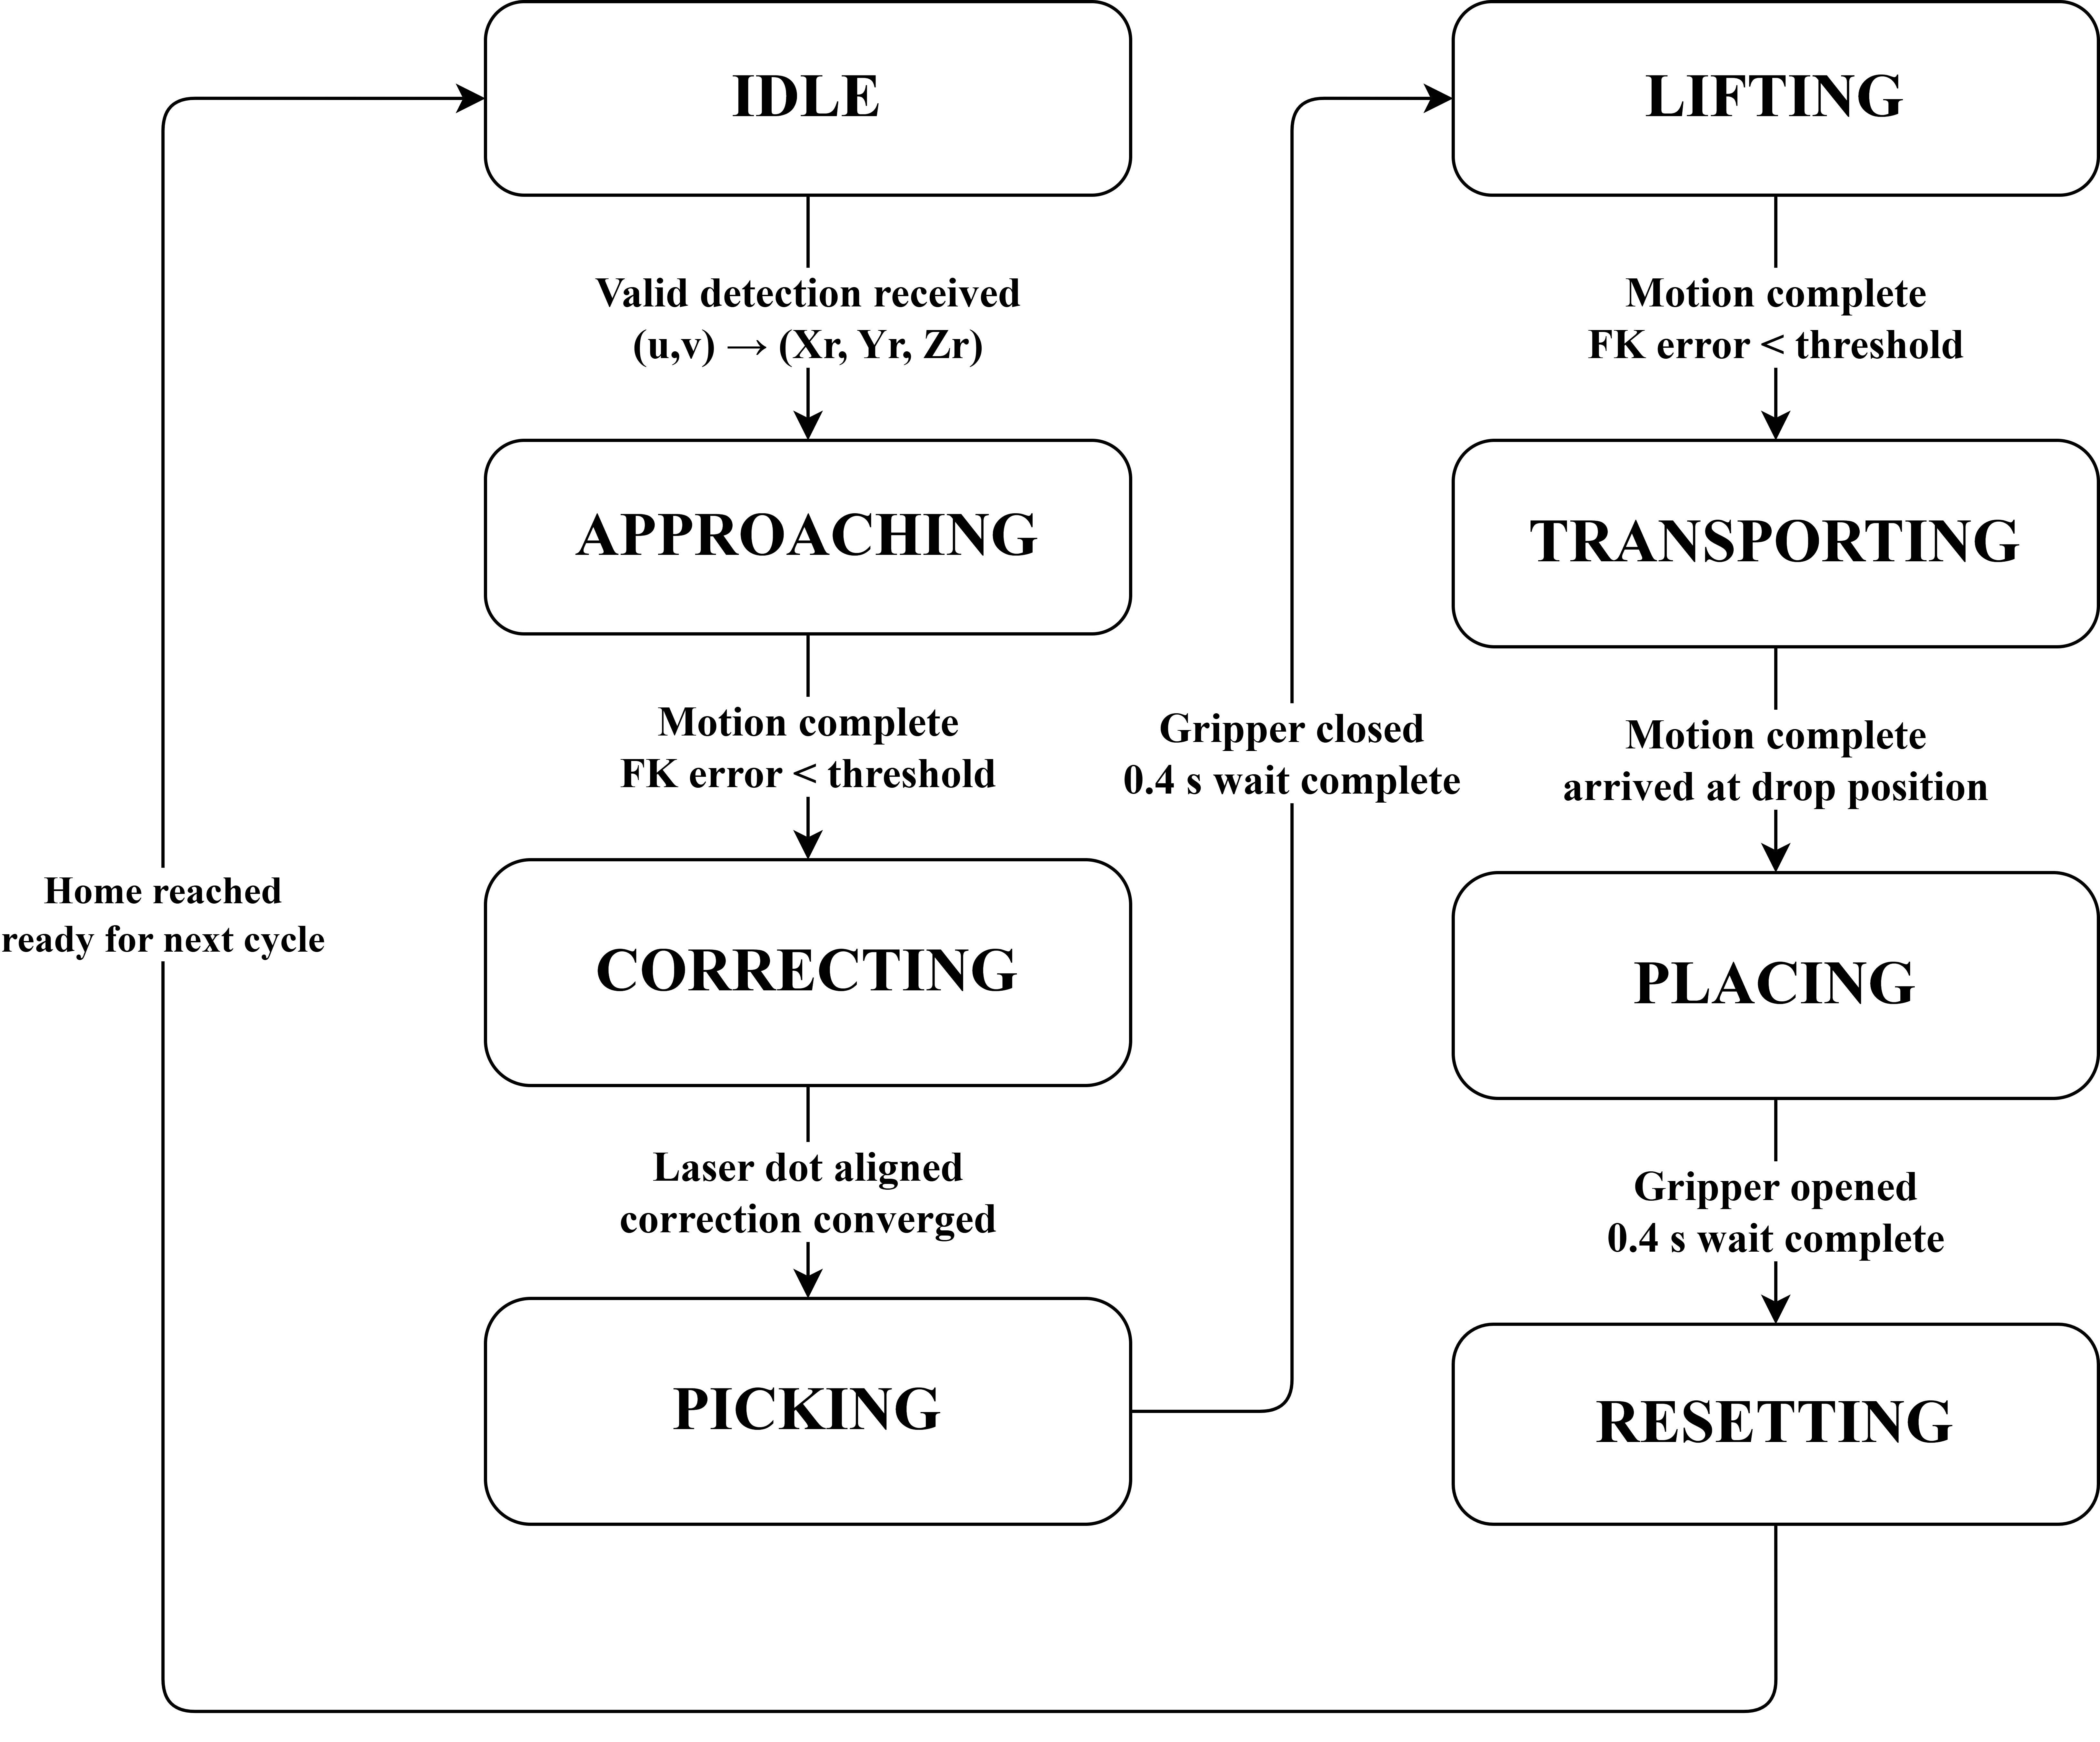
\includegraphics[width=0.45\linewidth]{image/fsm_pick_place.png}
    \caption{Pick-and-Place Finite State Machine (8 States).}
    \label{fig:task_framework}
\end{figure}

\hspace{1.27cm}
The sequence begins in \textbf{IDLE}, where the system
waits for a valid detection from the vision pipeline. Once
a detection is confirmed over \texttt{DETECTION\_CONFIRM\_FRAMES}
consecutive frames, the FSM enters \textbf{APPROACHING},
commanding the end-effector to move horizontally to the
target $(X_r,\, Y_r)$ at approach depth
$z_{\text{approach}} = Z_r$ (no vertical offset, $APPROACH\_Z\_OFFSET = 0$).
During this move, the visual end-effector feedforward correction
loop runs: it detects the laser dot, computes the horizontal offset
between the dot centroid and the object centroid, and issues
iterative position corrections until the X-axis error falls
below \texttt{EE\_CORRECTION\_THRESH\_MM = 3}\,mm. Once
aligned, the FSM transitions to \textbf{PICKING}, descending
to the pick depth $Z_{\text{pick}} = -535$\,mm (platform Z,
corresponding to EE tip at the belt surface), and the
\textbf{GRASPING} state activates the pneumatic gripper,
followed by a 0.4\,s dwell to allow the jaw to fully engage.
The robot then enters \textbf{LIFTING}, ascending to a safe
clearance height of $z_{\text{pick}} + 30$\,mm, before entering
\textbf{TRANSPORTING}, which moves the end-effector horizontally
to the drop position $(150,\, -150,\, -500)$\,mm (platform Z)
at the belt exit. In the \textbf{DROPPING} state the gripper
opens and a 0.4\,s dwell ensures the object is released before
the robot enters \textbf{RESETTING}, returning to the home
position $(0,\, 0,\, -350)$\,mm and transitioning back to IDLE
for the next pick cycle.

%--------------------------------------------------------------------
\subsubsection{Trajectory Planning Algorithm}
\hspace{1.27cm}
Trajectories between Cartesian waypoints are planned using
a triangular velocity profile, which applies when the
travel distance is shorter than the distance required to
reach $v_{\max}$. For the medium motion preset
($v_{\max} = 2000$\,mm/s, $a_{\max} = 5000$\,mm/s$^2$),
the minimum distance required to reach $v_{\max}$ is:

\begin{cequation}
    d_{\text{accel}} = \frac{v_{\max}^2}{2\, a_{\max}}
    = \frac{2000^2}{2 \times 5000} = 400\,\text{mm}.
    \label{eq:daccel}
\end{cequation}

Since all moves within the $\pm$150\,mm workspace are
shorter than $2 \times 400 = 800$\,mm, all trajectories
use the triangular profile, and the travel time for a move
of distance $d$ is:

\begin{cequation}
    t_{\text{move}} = 2\sqrt{\frac{d}{a_{\max}}}.
    \label{eq:tmove}
\end{cequation}

Intermediate Cartesian waypoints are generated by linear
interpolation at time steps of $\Delta t = 0.05$\,s, and
the IK solver is evaluated at each waypoint to produce a
sequence of joint angle commands sent to the motors over
the CAN bus.

%============================================================================
\subsection{Calibration Procedure}\label{sec:calibration}
\hspace{1.27cm}
Before operation, the camera-to-robot coordinate transform
is calibrated to align the projected workspace overlay with
the physical robot workspace. The calibration uses a visual
reference: a white crosshair marker is rendered in the
camera feed at the projected base-frame origin
$(0,\, 0,\, -650)$\,mm. The calibration sequence is as
follows:

\begin{enumerate}
    \item Command the robot to the home position
    $(0,\, 0,\, -350)$\,mm. The red laser dot on the
    end-effector tip indicates the physical robot origin
    projected onto the belt surface in the camera image.

    \item Observe the offset between the crosshair
    position and the laser dot centroid in the live
    camera feed.

    \item Adjust \texttt{CAM\_TX\_MM} in $\pm$10\,mm
    steps until the crosshair aligns horizontally with
    the laser dot.

    \item Adjust \texttt{CAM\_TY\_MM} in $\pm$10\,mm
    steps until the crosshair aligns vertically with
    the laser dot.

    \item Verify calibration by placing a physical object
    at the robot kinematic centre $(0,\, 0)$ and
    confirming that the system reports
    \texttt{BASE = (0, 0, -650)} within $\pm$5\,mm.
\end{enumerate}

\begin{figure}[h]
    \centering
    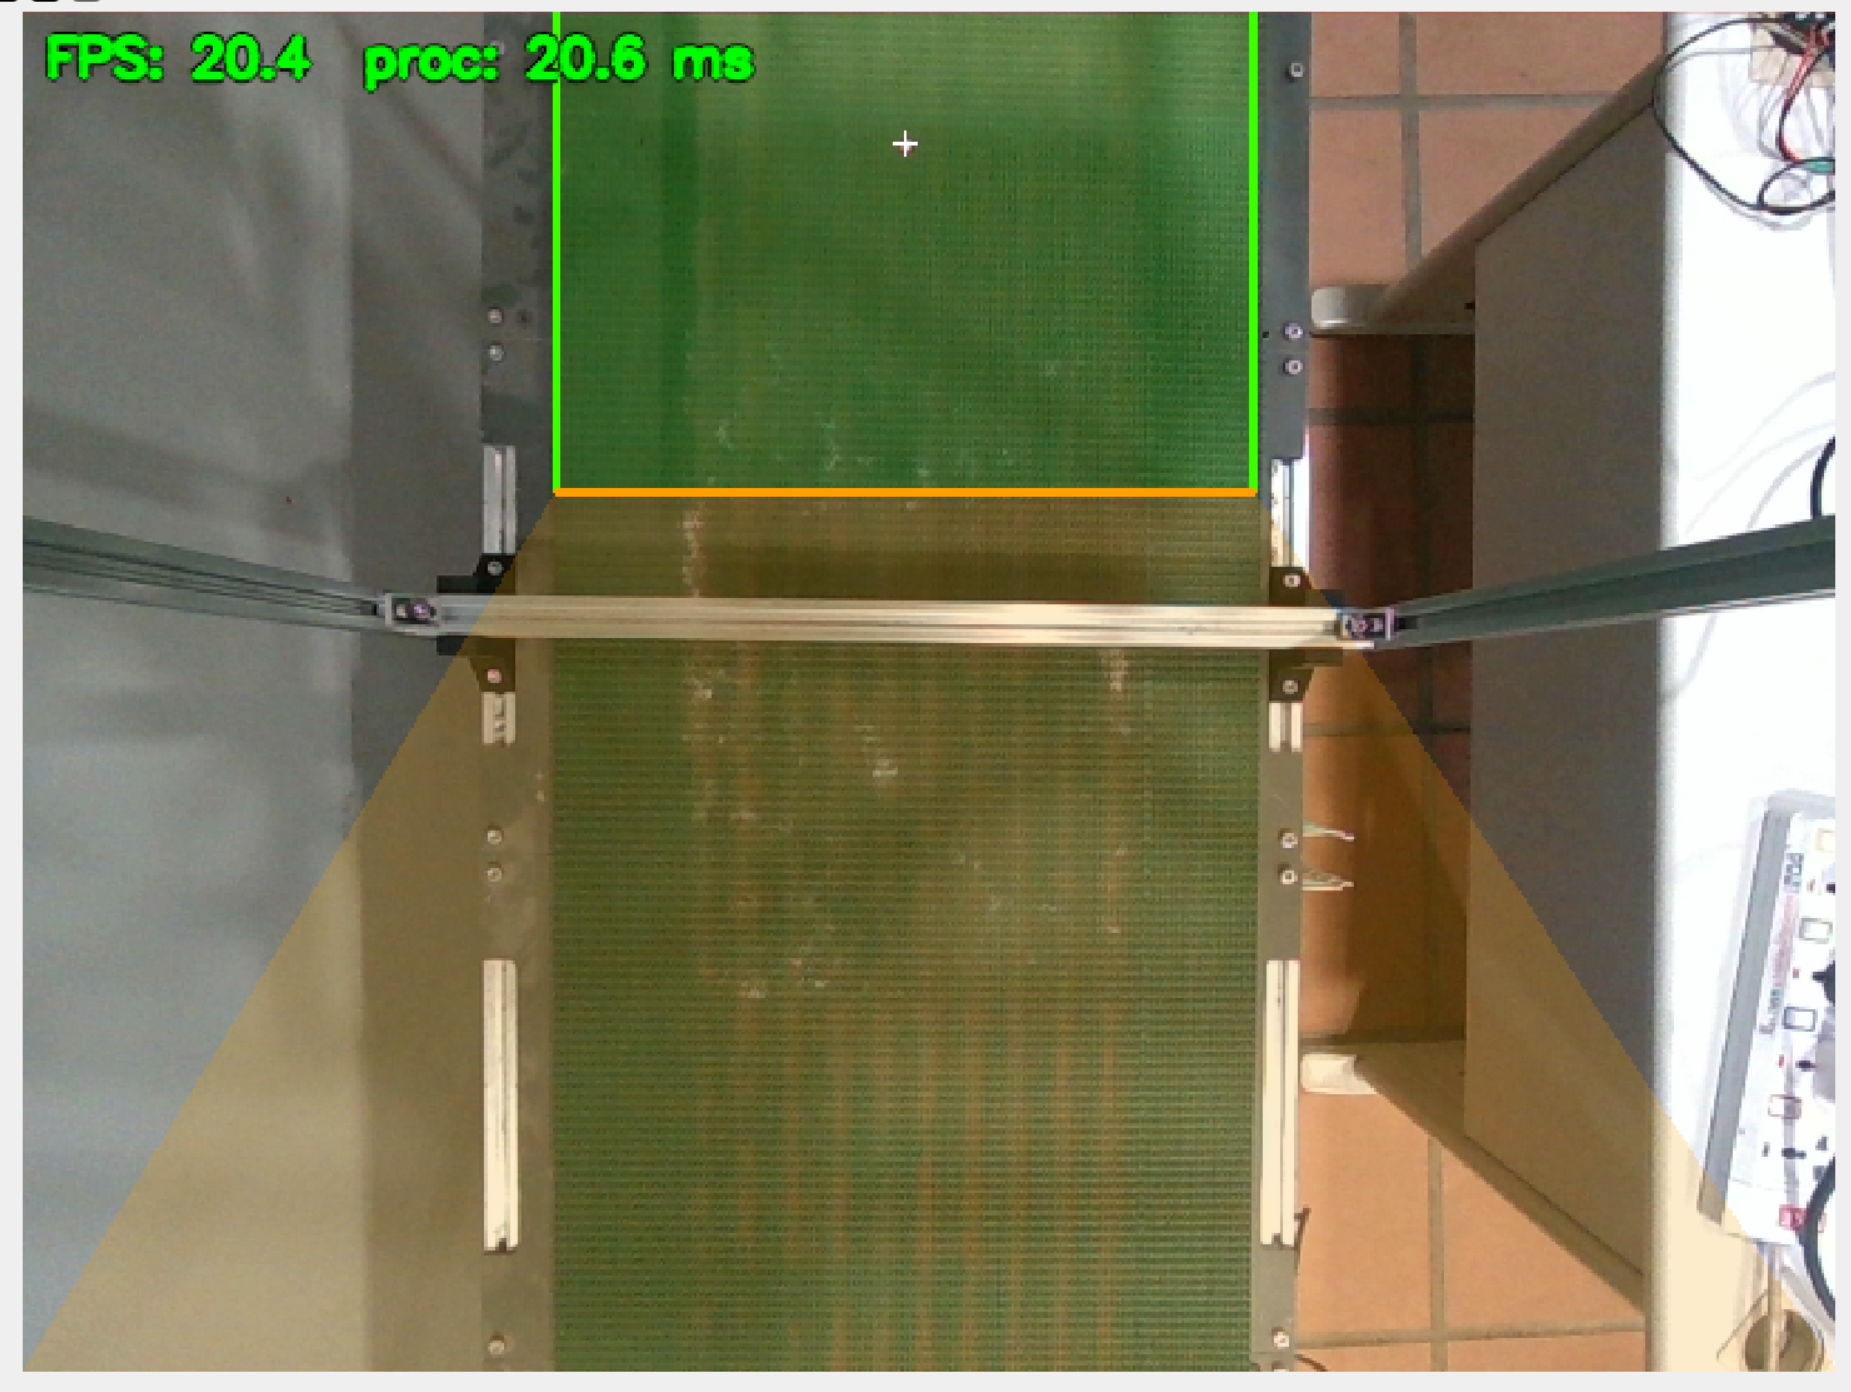
\includegraphics[width=0.5\linewidth]{image/Calibrate WorkSpace.png}
    \caption{Camera calibration: crosshair aligned to the
             end-effector laser dot at the robot kinematic
             origin.}
    \label{fig:calibration_gui}
\end{figure}

\hspace{1.27cm}
The calibrated translation vector for this system is
$\mathbf{t} = [-10.0,\; +235.0,\; -20.0]^{\top}$\,mm.
The parameters \texttt{CAM\_TX\_MM = -10.0}\,mm and
\texttt{CAM\_TY\_MM = 235.0}\,mm are the horizontal X and Y
offsets of the camera optical centre relative to the robot base
frame origin, determined empirically. The parameter
\texttt{CAM\_TZ\_MM = -20.0}\,mm indicates that the camera is
mounted 20\,mm below the robot base frame origin along the
$Z$-axis. The camera-to-belt vertical distance used in the
pinhole backprojection is stored separately as
\texttt{FAKE\_DEPTH\_M = 0.650}\,m (650\,mm), which is the
measured vertical distance from the camera optical centre to
the belt surface at the pick depth.

%============================================================================
\subsection{Vision Pipeline}
\hspace{1.27cm}
The vision pipeline converts raw RGB camera data into robot
base-frame coordinates used by the motion controller. It
consists of four sequential stages as illustrated in
\textbf{\autoref{fig:vision_pipeline}}. The pipeline is
triggered once per incoming colour frame at 15--30\,fps and
produces a validated target position $(X_r,\, Y_r,\, Z_r)$
that is published to the \texttt{/target\_robot\_xyz} topic
for consumption by the IK solver, or discards the frame
silently if any stage fails its validity check.

\begin{figure}[h]
    \centering
    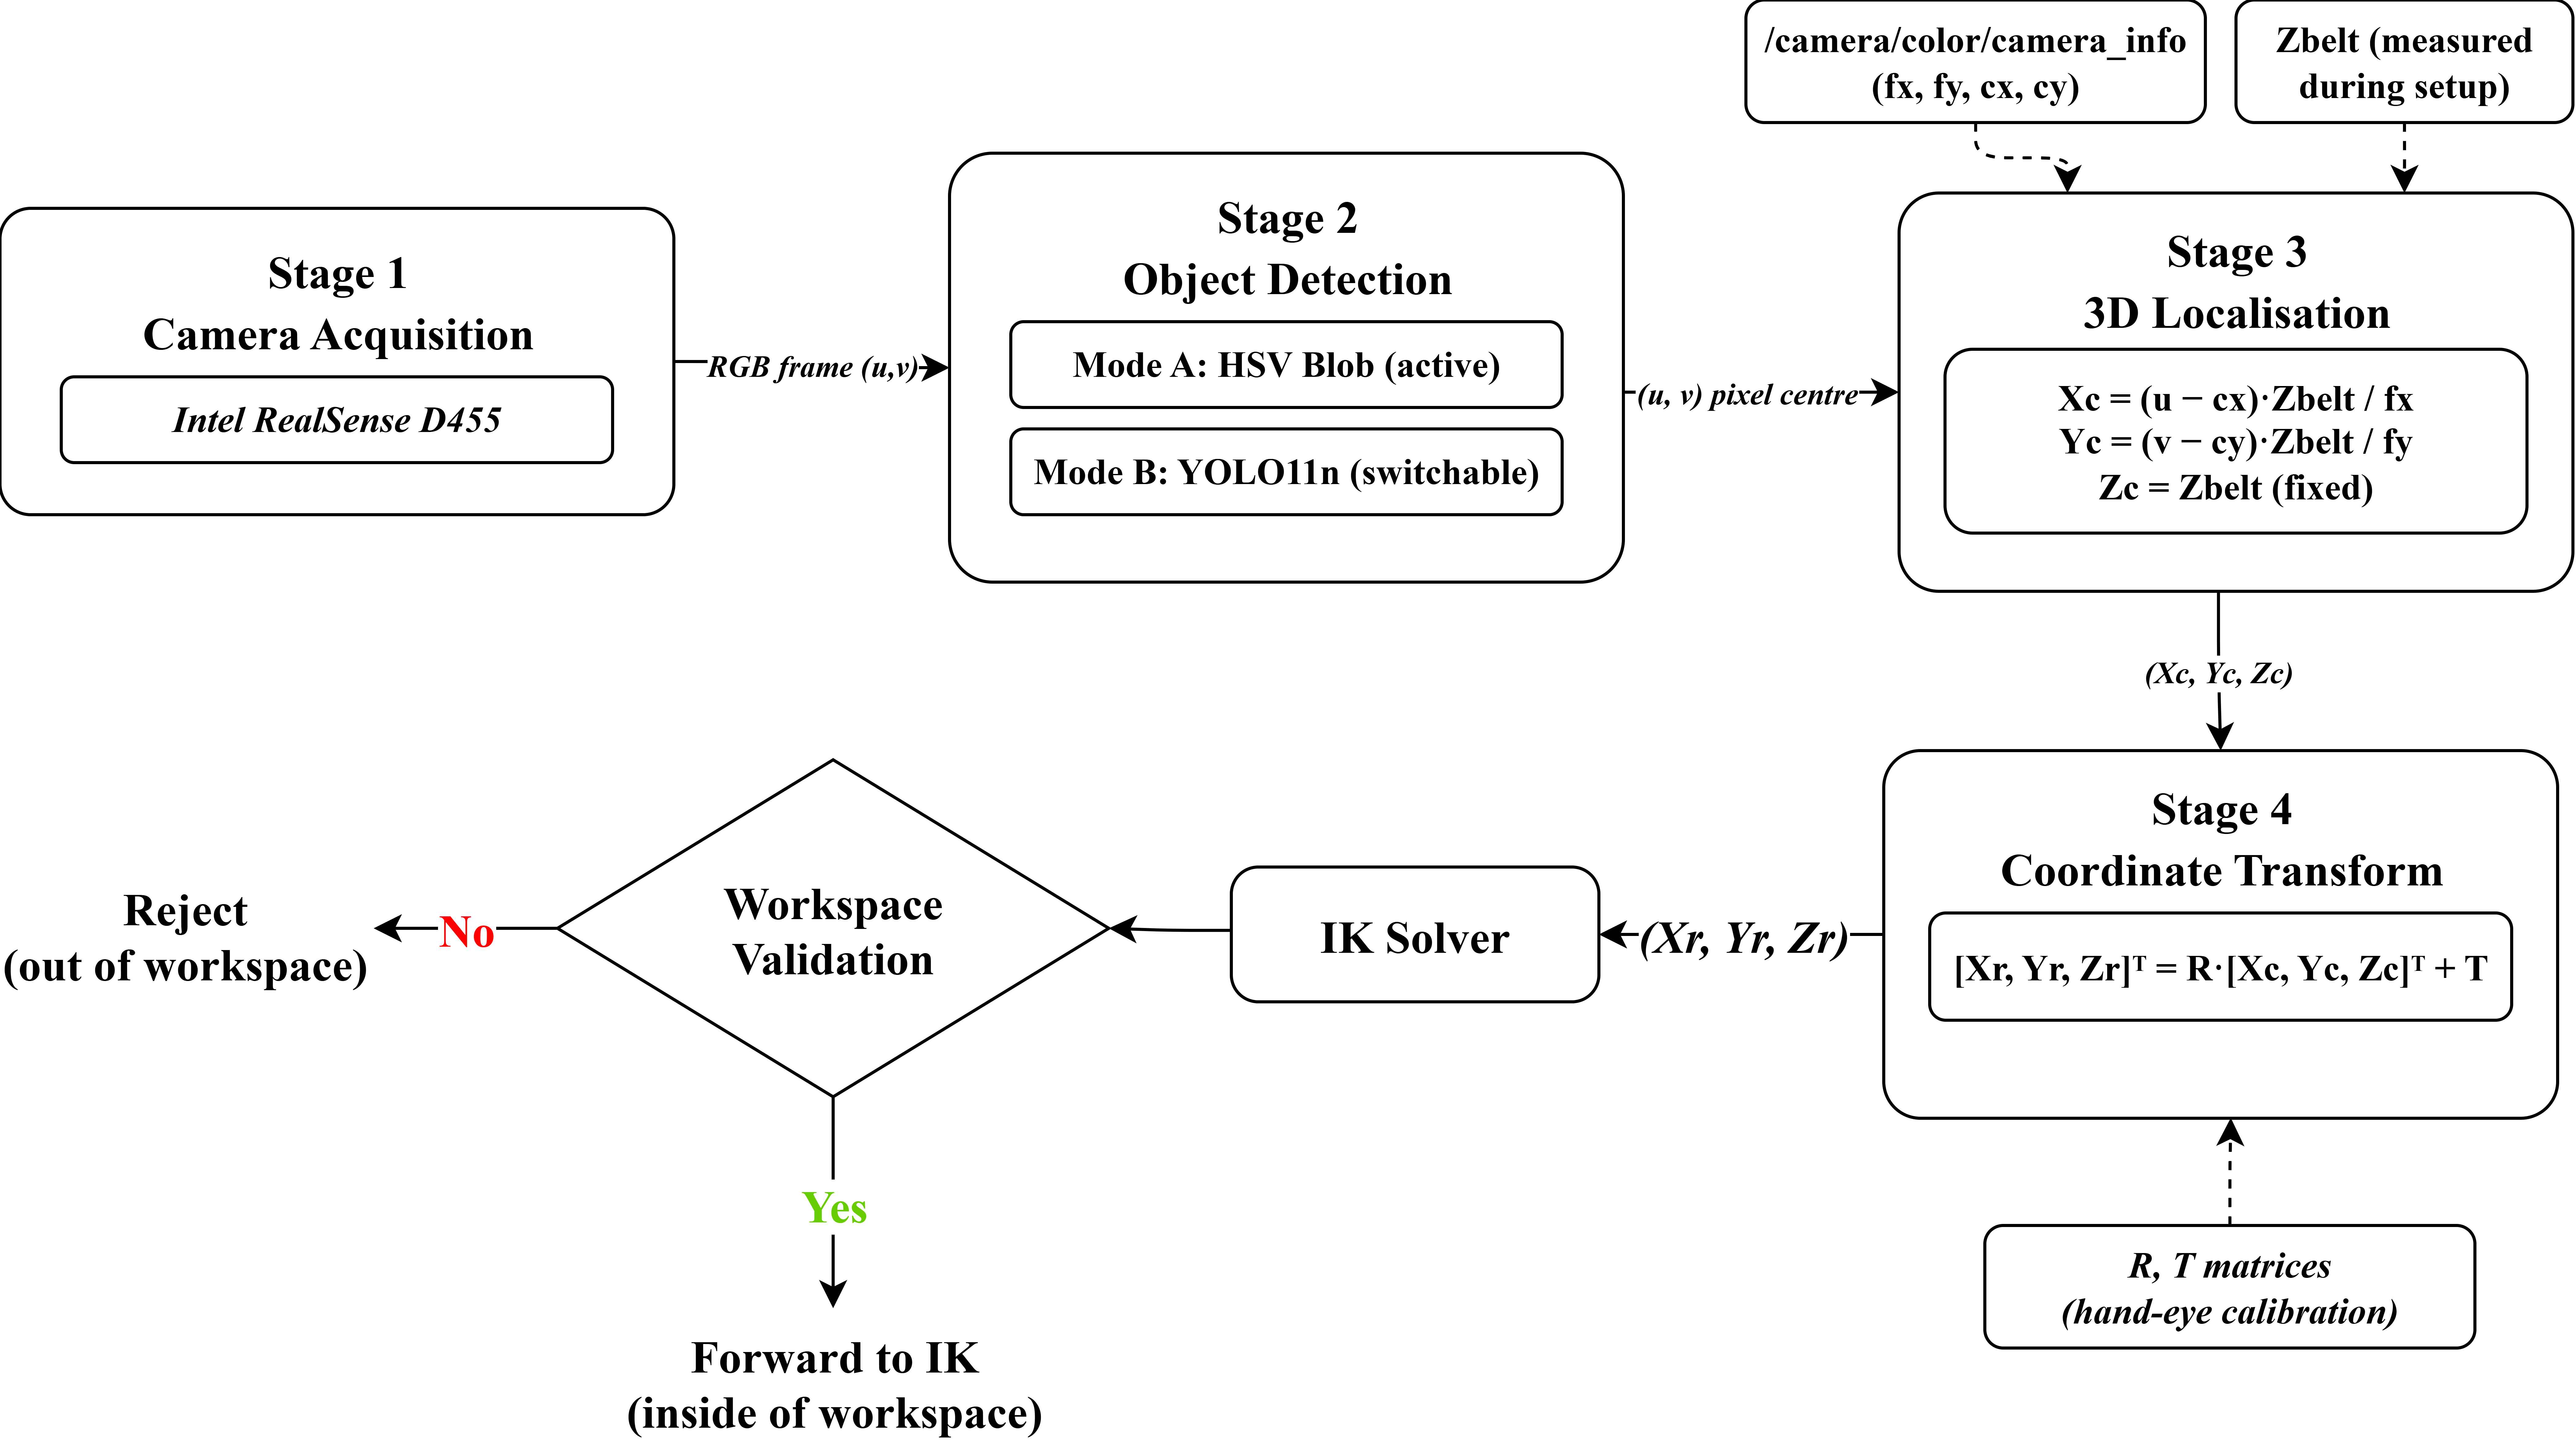
\includegraphics[width=0.72\linewidth]{image/vision_pipeline.png}
    \caption{Vision-to-Motion Pipeline: Stage Architecture.}
    \label{fig:vision_pipeline}
\end{figure}

%--------------------------------------------------------------------
\subsubsection{Camera Hardware and ROS~2 Topics}
\hspace{1.27cm}
The Intel RealSense D455 camera is mounted overhead,
directed vertically downward at the workspace. Although the
D455 is capable of stereo depth sensing with a 95\,mm
baseline and structured infrared illumination, only its RGB
colour stream is used in this system. The conveyor belt
surface lies at a fixed and known elevation of approximately
$Z_{\text{belt}} = -650$\,mm below the robot base frame (EE-tip
coordinate; platform Z at pick $= -535$\,mm),
so per-pixel depth measurement is unnecessary: the $Z$
coordinate of every pick target is constant by
construction, eliminating the need to process the depth
stream entirely and reducing pipeline latency. The camera
provides the following ROS~2 topics consumed by the
detection node:

\begin{itemize}
    \item \texttt{/camera/camera/color/image\_raw}:
    RGB image at $640 \times 480$\,px, 30\,fps,
    published as \texttt{sensor\_msgs/Image} in BGR8
    encoding.
    \item \texttt{/camera/camera/color/camera\_info}:
    camera intrinsic matrix $\mathbf{K}$ containing
    focal lengths $(f_x,\, f_y)$ and principal-point
    coordinates $(c_x,\, c_y)$, read once at node
    startup and cached for the session.
\end{itemize}

\hspace{1.27cm}
Reading the intrinsic parameters live from the
\texttt{camera\_info} topic rather than a static
configuration file ensures that the correct calibration
is used regardless of any change in camera resolution or
mounting position, since the RealSense driver recomputes
and republishes intrinsics appropriate to the active
stream profile on every startup.

%--------------------------------------------------------------------
\subsubsection{Object Detection}
\hspace{1.27cm}
Object detection is performed by a configurable detection
node that supports two interchangeable modes, selected
via the \texttt{DETECTION\_MODE} parameter in
\texttt{config.py}. Both modes produce the same output
interface: a single pixel coordinate $(u,\, v)$
representing the centroid of the detected target object.
The live camera feed with all overlays active is shown
in \textbf{\autoref{fig:detection_feed}}, where the
system is running at 30\,fps with a processing latency
of 5.3\,ms per frame.
\begin{figure}[h]
    \centering
    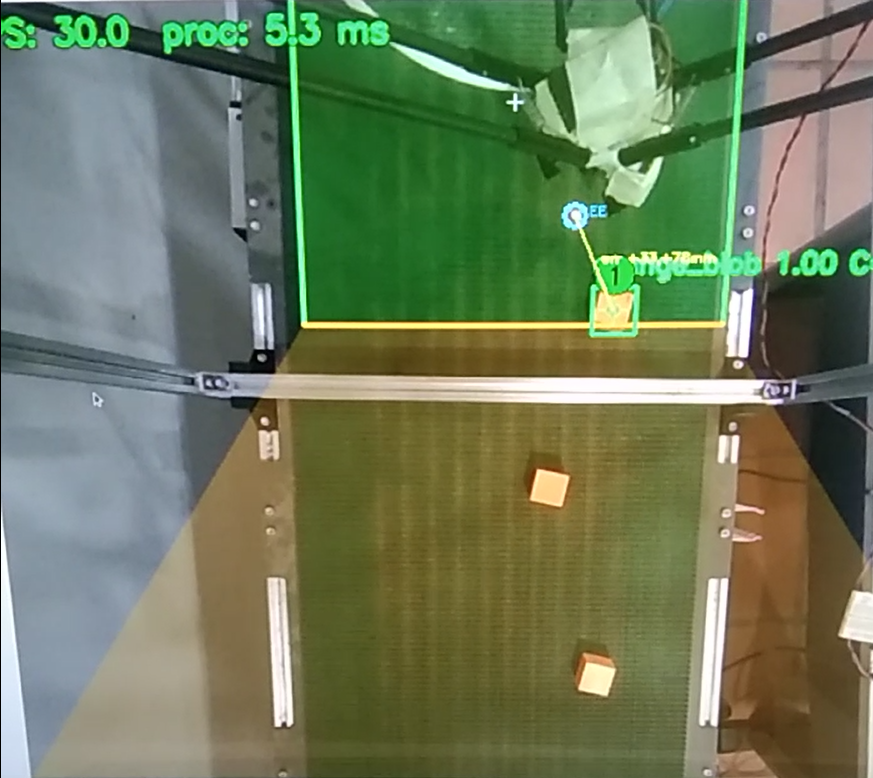
\includegraphics[width=0.55\linewidth]{image/EE and obj detection.png}
    \caption{Live camera feed from the RealSense D455
             during active pick-and-place operation at
             30\,fps (proc: 5.3\,ms). The green rectangle
             marks the operational workspace boundary. The
             detected orange cube is enclosed by a green
             bounding box labelled \texttt{orange\_blob}
             with confidence 1.00. The cyan \texttt{EE}
             circle indicates the projected end-effector
             laser dot position, connected by a yellow
             offset line to the object centroid showing
             the active EE correction residual. The yellow
             horizontal line is the belt prediction
             overlay. Two additional orange cubes are
             visible on the belt outside the workspace
             boundary and are correctly ignored by the
             detection node.}
    \label{fig:detection_feed}
\end{figure}


\par
\hspace{1.27cm}
\textbf{orange\_blob mode (active).} HSV colour-space
filtering detects the target object by applying a
dual-range hue threshold tuned to the orange target
colour. The algorithm converts each incoming BGR frame
to HSV, applies the threshold masks, and identifies the
largest valid contour in the resulting binary image. The
centroid of this contour is computed using image moments
and returned as the pixel coordinate $(u,\, v)$. As
visible in \textbf{\autoref{fig:detection_feed}}, the
detected orange cube is enclosed by a green bounding box
and labelled \texttt{orange\_blob} with a detection
confidence of 1.00, confirming reliable detection under
the controlled green-screen background of the workspace.
This mode achieves 30\,fps on CPU with a processing time
of 5.3\,ms per frame and zero model loading overhead,
providing deterministic, low-latency detection under
controlled lighting conditions.

\par
\hspace{1.27cm}
\textbf{yolo mode (implemented, switchable).}
YOLO11n (\texttt{yolo11n.pt}, Ultralytics) provides
deep learning-based object detection. The bounding box
centre of the highest-confidence detection above the
configured score threshold is used as the pixel
coordinate $(u,\, v)$. This mode requires the trained
weights file to be present and a configured target class
index in \texttt{config.py}. It is integrated and ready
for activation but was not used for primary system
validation due to its higher CPU inference latency
compared to the HSV mode.

\par
\hspace{1.27cm}
The camera feed in \textbf{\autoref{fig:detection_feed}}
also shows three additional overlays generated by the
detection node. The \textbf{green rectangle} defines the
operational workspace boundary within the camera field of
view: only objects whose detected centroids fall inside
this boundary are forwarded to the coordinate transform
stage. The \textbf{yellow horizontal line} is the belt
prediction overlay, representing the estimated conveyor
belt position at the future pick instant computed by the
belt prediction node. The \textbf{cyan circle} labelled
\texttt{EE} marks the current projected position of the
end-effector laser dot on the belt surface as tracked by
the visual correction loop, and the yellow connecting line
drawn from the \texttt{EE} marker to the detected object
centroid represents the residual offset $(\Delta u,\,
\Delta v)$ that the EE feedforward correction loop is
actively minimising. Frames for which no valid detection
is returned, either because no object is present within
the workspace boundary, the detected contour area falls
below the minimum size threshold, or the YOLO confidence
is below the minimum score, are discarded without
publishing any target, and the pipeline waits for the
next frame.


%--------------------------------------------------------------------
\subsubsection{Pixel-to-Camera-Frame Conversion}
\hspace{1.27cm}
Given the detected pixel coordinate $(u,\, v)$ and the
camera intrinsic parameters $(f_x,\, f_y,\, c_x,\, c_y)$
read from the \texttt{camera\_info} topic, the
corresponding 3D point in the camera coordinate frame is
computed using the fixed-height backprojection derived
from the pinhole camera model \autocite{hartley-2004}:

\begin{cequation}
    X_c = \frac{(u - c_x)}{f_x} \cdot Z_{\text{fixed}},
    \qquad
    Y_c = \frac{(v - c_y)}{f_y} \cdot Z_{\text{fixed}},
    \qquad
    Z_c = Z_{\text{fixed}},
    \label{eq:pixel_to_cam}
\end{cequation}

where $Z_{\text{fixed}}$ is stored as the configuration
parameter \texttt{FAKE\_DEPTH\_M = 0.650\,m} (650\,mm) and
represents the measured vertical distance from the camera
optical centre to the belt surface. This conversion is valid
because all pick targets rest on the conveyor belt at a
constant known depth below the camera, so the fixed-$Z$
assumption holds for every frame without exception. No depth
image or per-frame depth measurement is required.

%--------------------------------------------------------------------
\subsubsection{Camera-to-Robot Frame Transform}\label{sec:coordinate_transform}
\hspace{1.27cm}
The camera-frame 3D point
$\mathbf{p}_c = [X_c,\, Y_c,\, Z_c]^{\top}$ is mapped to
the robot base frame through the calibrated rigid-body
transformation \autocite{tsai-lenz-1989}:

\begin{cequation}
    \mathbf{p}_{\text{base}}
    = \mathbf{R}\, \mathbf{p}_c + \mathbf{t},
    \label{eq:transform_pipeline}
\end{cequation}

where the rotation matrix $\mathbf{R}$ encodes the axis
orientation and sign conventions between the two frames,
and the translation vector $\mathbf{t}$ encodes the
physical mounting offset of the camera optical centre
relative to the robot base-frame origin. The calibrated
values used in this system are:

\begin{cequation}
    \mathbf{R} =
    \begin{bmatrix}
        -1 & 0 &  0 \\
         0 & 1 &  0 \\
         0 & 0 & -1
    \end{bmatrix},
    \qquad
    \mathbf{t} =
    \begin{bmatrix}
        -10.0 \\ +235.0 \\ -20.0
    \end{bmatrix} \text{mm}.
    \label{eq:R_and_t}
\end{cequation}

\hspace{1.27cm}
The $-1$ entries in $\mathbf{R}$ reflect the axis sign
inversions required to align the camera coordinate frame
(where the $X$-axis points right and $Z$ points into the
scene) with the robot base frame (where $X$ points in the
robot positive direction and $Z$ points downward from the
base). The diagonal structure confirms that no axis swap
is present: each robot-frame axis corresponds to exactly
one camera-frame axis with a possible sign flip. The
translation offsets $t_x = -10.0$\,mm,
$t_y = +235.0$\,mm, and $t_z = -20.0$\,mm were
determined during the empirical calibration procedure
described in \autoref{sec:calibration} by placing a
reference object at the robot kinematic centre and
iteratively adjusting the offsets until the reported
base-frame coordinates matched the known physical
position.

\par
\hspace{1.27cm}
The resulting robot base-frame coordinates
$(X_r,\, Y_r)$ from \autoref{eq:transform_pipeline} are
paired with the fixed pick height $Z_r = -535$\,mm (platform Z,
corresponding to EE tip at the belt surface) to
form the complete 3D target position
$(X_r,\, Y_r,\, -535)$\,mm, which is then subject to
workspace validation before being passed to the inverse
kinematics solver. The coordinate transform geometry and
the relationship between the camera and robot frames are
illustrated in \textbf{\autoref{fig:camera_transform}}.

\begin{figure}[h]
    \centering
    \includegraphics[width=0.50\linewidth]{image/coordernationTransform.png}
    \caption{Camera-to-Robot Coordinate Transform Diagram
             showing the axis relationships between the
             RealSense D455 camera frame and the Delta robot
             base frame, with the calibrated rotation matrix
             $\mathbf{R}$ and translation $\mathbf{t}$
             annotated.}
    \label{fig:camera_transform}
\end{figure}

%--------------------------------------------------------------------
\subsubsection{Workspace Validation}
\hspace{1.27cm}
Before the target coordinate is published to the
controller, the robot-frame position
$(X_r,\, Y_r,\, Z_r)$ is checked against the operational
workspace bounds defined in \autoref{tab:workspace}:

\begin{itemize}
    \item $|X_r| \leq 150$\,mm
    \item $|Y_r| \leq 150$\,mm
    \item $Z_{\min} \leq Z_r \leq Z_{\max}$
\end{itemize}

\hspace{1.27cm}
Any target position that violates any of these constraints
is discarded and a warning is logged to the ROS~2 console.
Only positions that pass all three checks are published on
the \texttt{/target\_robot\_xyz} topic as a
\texttt{geometry\_msgs/Point} message and consumed by the
FSM controller node as the IK input target. This safety
layer prevents the IK solver from being invoked on
geometrically unreachable positions and protects the
mechanical structure from commands that would drive the
arms into a singular or over-extended configuration.

%============================================================================
% END OF SECTION
%============================================================================
%============================================================================
% END OF VISION PIPELINE SECTION
%============================================================================

\subsection{ROS\,2 System Architecture}
\hspace{1.27cm}
The complete system is implemented as five ROS\,2 packages communicating via topics and services, as shown in \textbf{\autoref{fig:ros2_architecture}}.

\par
\begin{figure}[h]
    \centering
    \includegraphics[width=1.0\linewidth]{image/ros2_architecture_wiring-ROS 2 System Architecture.png}
    \caption{ROS\,2 System Architecture Node and Topic Graph.}
    \label{fig:ros2_architecture}
\end{figure}



  \section{RESULTS AND DISCUSSION}

%============================================================================
\subsection{Hardware Assembly}
\hspace{1.27cm}
The hardware assembly phase involved the integration of all mechanical, electrical, and control components to form the complete Delta robot system. This stage validated the design decisions made during the methodology phase and prepared the robot for testing.

\subsubsection{Mechanical Assembly}
\hspace{1.27cm}
The Delta robot frame was assembled using aluminum profiles for the fixed base and 3D-printed PLA parts for the arm linkages and moving platform. The three upper arms (length $r_f = 200$\,mm) are connected to the RobStride RS-00 motor shafts via custom motor mounts. The lower arm parallelograms (length $r_e = 400$\,mm) use ball joints at both ends to allow free rotation while constraining the moving platform to pure translational motion. The moving platform (side $e = 35$\,mm) carries the pneumatic solenoid gripper. The fixed base triangle (side $f = 157$\,mm) provides the reference coordinate frame for all kinematic calculations.

\par
\begin{figure}[h]
    \centering
    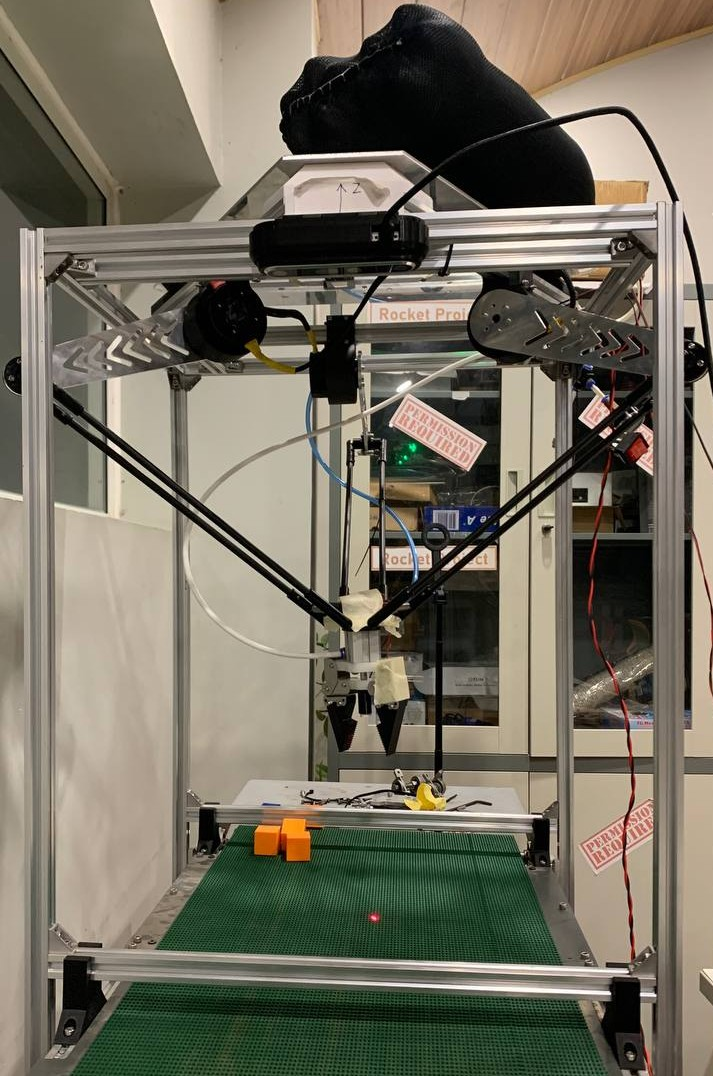
\includegraphics[width=0.45\linewidth]{image/completedAssemblied.jpg}
    \hfill
    \includegraphics[width=0.45\linewidth]{image/completedAssem.png}
    \caption{Delta Robot Complete Assembly: fabricated prototype (left)
             and CAD reference (right).}
    \label{fig:robot_assembly}
\end{figure}

\subsubsection{Electrical and Control Assembly}
\hspace{1.27cm}
Three RobStride RS-00 quasi-direct-drive motors (CAN IDs 1, 2, 3) are connected in a CAN bus daisy chain at 1\,Mbit/s. A USB-to-CAN adapter (SocketCAN, \texttt{can0}) interfaces the motors to the host computer. The pneumatic solenoid gripper is driven by motor driver CAN ID\,4 (open: \texttt{004\#00}, close: \texttt{004\#01}). The Intel RealSense D455 camera is connected via USB\,3.0 and powered independently. A 24\,V power supply feeds the motor drivers; the host computer runs Ubuntu 22.04 with ROS\,2 Humble.

\par
\begin{figure}[h]
    \centering
    % \includegraphics[width=0.7\linewidth]{image/electronics_assembly.jpg}
    \caption{Electronics and CAN Bus Assembly.}
    \label{fig:electronics_assembly}
\end{figure}

%============================================================================
\subsection{Kinematic Validation}
\hspace{1.27cm}
The kinematic model was validated by commanding the robot to a set of known positions and comparing the FK-computed end-effector position against the commanded position.

\subsubsection{Forward Kinematics Validation}
\hspace{1.27cm}
For each commanded position $(x, y, z)$, the IK solver computed joint angles $(\theta_1, \theta_2, \theta_3)$, which were sent to the motors. Motor encoder feedback was read back, FK was applied to the measured angles, and the position error was computed. Results from a representative set of test positions are shown in \textbf{\autoref{tab:fk_validation}}.

\begin{table}[ht]
    \centering
    \caption{Forward Kinematics Validation Results.}
    \label{tab:fk_validation}
    \small{
    \begin{tabular}{ccccccccc}
        \textbf{Test} & $\theta_1$($^\circ$) & $\theta_2$($^\circ$) & $\theta_3$($^\circ$) & $x$ (mm) & $y$ (mm) & $z$ (mm) & \textbf{FK err} (mm) \\
        \hline
        1 & 7.3  & 7.3  & 7.3  &   0.0 &    0.0 & $-$350.0 & 0.39 \\
        2 & 22.4 & 22.4 & 22.4 &   0.0 &    0.0 & $-$410.0 & 0.36 \\
        3 & 26.2 & 12.1 & 36.3 &  88.0 &    6.0 & $-$410.0 & 0.44 \\
        4 & 34.2 & 15.0 &  8.2 & $-$22.5 & 91.4 & $-$385.0 & 0.47 \\
        5 & 5.4  & 42.1 & 42.1 &   0.0 & $-$150.0 & $-$410.0 & 0.45 \\
        6 & 30.1 &  9.0 & 43.9 & 127.5 &  10.5 & $-$410.0 & 0.39 \\
        \ChangeRT{1.5pt}
    \end{tabular}}
\end{table}

\hspace{1.27cm}
FK position errors were consistently below 0.5\,mm across all tested configurations, confirming that the kinematic model is accurate and the motor encoder feedback is reliable. The maximum observed error of 0.47\,mm is well within the tolerance required for pick-and-place operations with the pneumatic gripper.

\subsubsection{Inverse Kinematics Validation}
\hspace{1.27cm}
IK solutions were pre-checked before every pick sequence. All approach, pick, lift, and home positions were verified reachable (IK status = 0) before commanding any motion. The joint angle constraint $\theta_i \geq 0$ was enforced to prevent physically unreachable configurations. No IK failures were observed during normal operation within the $\pm150$\,mm planar workspace at pick depth $Z = -410$\,mm.

%============================================================================
\subsection{Vision Pipeline Results}

\subsubsection{Camera Calibration}
\hspace{1.27cm}
Camera-to-robot transform calibration was performed iteratively using a projected workspace overlay rendered in the camera feed. The overlay projects the four workspace corners (at $(\pm150, \pm150, -490)$\,mm platform frame) through the inverse transform to image pixels, drawing the green workspace box and a white crosshair at the projected $(0, 0)$ origin. By adjusting \texttt{CAM\_TX\_MM = -10.0}\,mm and \texttt{CAM\_TY\_MM = +235.0}\,mm until the crosshair aligned with the laser dot at the robot home position, the transform was calibrated. The calibrated translation vector is:
\begin{equation*}
    \mathbf{t} = [-10.0,\; +235.0,\; -20.0]^\top \text{ mm}.
\end{equation*}

\subsubsection{Object Detection}
\hspace{1.27cm}
The HSV orange\_blob detector achieved consistent detection 
with a reported confidence of 1.00 across all tested 
lighting conditions, with a processing time of 3--16\,ms 
per frame at 13--31\,fps on CPU. The deterministic nature 
of HSV filtering provided zero false positives for the 
orange test object against the green cutting mat background.


%============================================================================
\subsection{Pick-and-Place Task}
\hspace{1.27cm}
A complete pick-and-place operation was performed to evaluate the performance of the developed Delta robot. The task involved detecting a stationary orange object, applying the visual EE feedforward correction loop, descending to pick depth ($Z_{\text{pick}} = -535$\,mm platform), grasping, transporting to the drop position at $(150,\, -150,\, -500)$\,mm platform (belt exit), and returning to home.

\par
\hspace{1.27cm}
The 8-state FSM executed the full sequence:
IDLE $\to$ APPROACHING $\to$ PICKING $\to$ GRASPING $\to$ LIFTING $\to$ TRANSPORTING $\to$ DROPPING $\to$ RESETTING $\to$ IDLE,
consistent with the FSM described in \autoref{sec:task_framework}.
\begin{figure}[h]
    \centering
    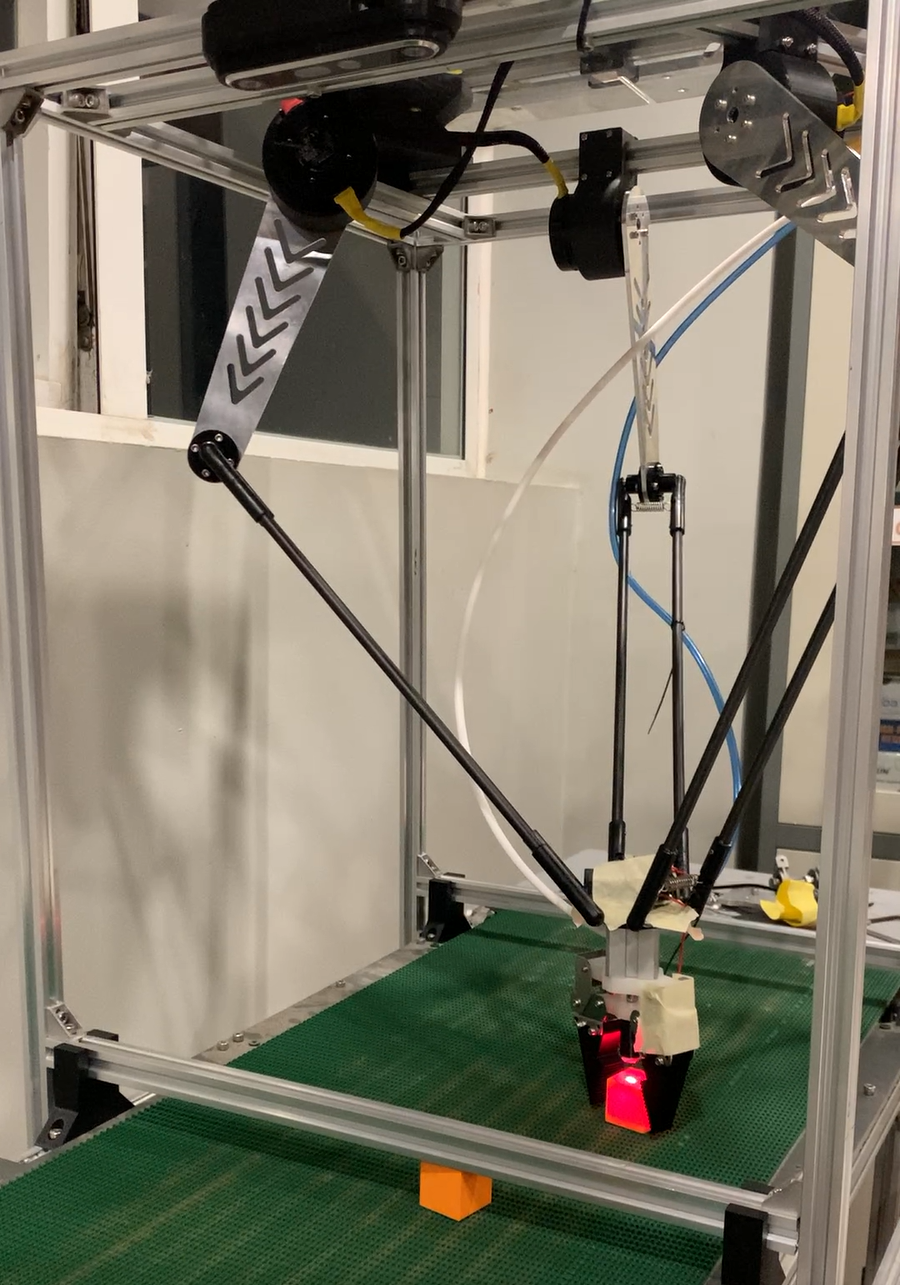
\includegraphics[height=6.5cm]{image/picking.png}
    \hspace{5mm}
    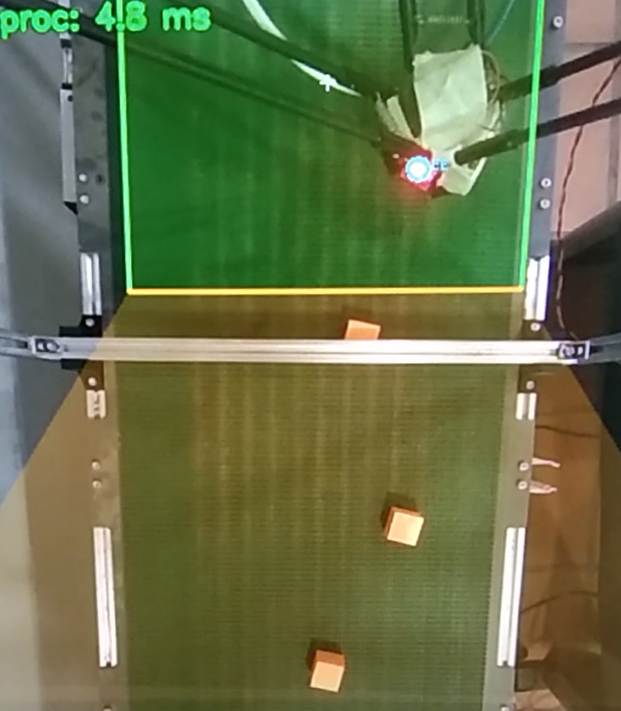
\includegraphics[height=6.5cm]{image/vspicking.png}
    \caption{Robot EE Approaching Object with Visual Correction Active:
             Physical Picking (left) and Visualization EE Correction
             Picking (right).}
    \label{fig:pick_task}
\end{figure}

\begin{figure}[h]
    \centering
    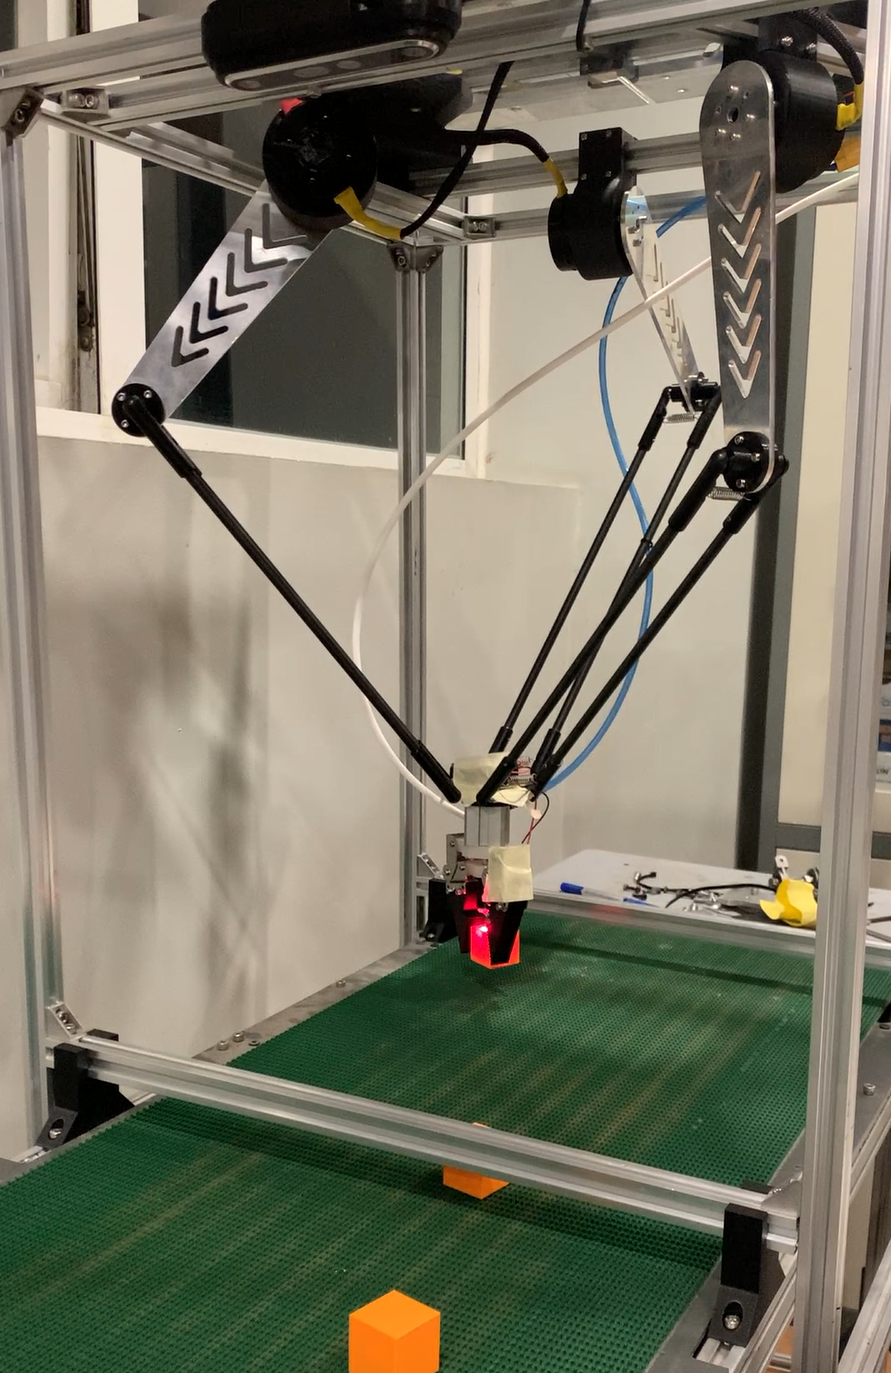
\includegraphics[height=6.5cm]{image/placing.png}
    \hspace{5mm}
    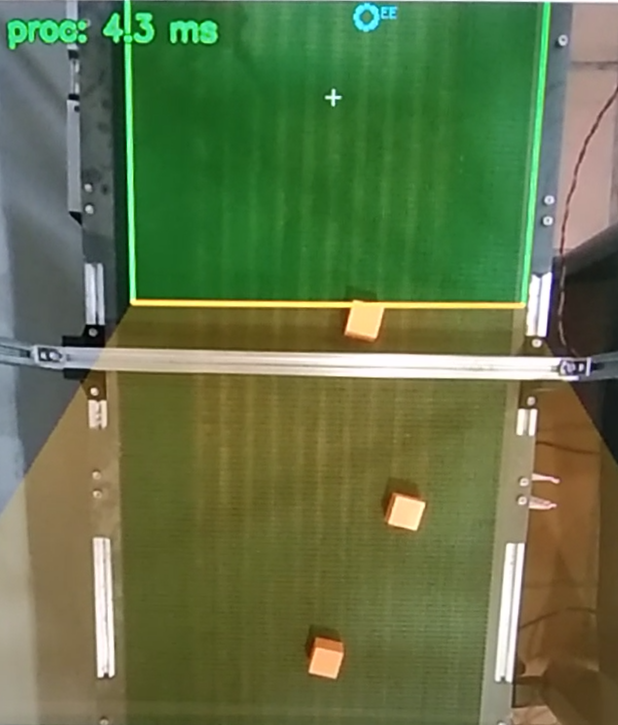
\includegraphics[height=6.5cm]{image/vsplacing.png}
    \caption{Robot Placing Object at Belt Exit Position: Physical
             Placing (left) and Visualization EE Correction
             Placing (right).}
    \label{fig:place_task}
\end{figure}

\subsubsection{Visual EE Correction Results}
\hspace{1.27cm}
The feedforward correction loop successfully reduced the X-axis error from an initial value of approximately 17--40\,mm to below the 3\,mm convergence threshold (\texttt{EE\_CORRECTION\_THRESH\_MM = 3.0}) within 2--4 iterations. A representative correction sequence is shown below:

\begin{table}[ht]
    \centering
    \caption{Representative EE Correction Iteration Results.}
    \label{tab:ee_correction_results}
    {\small
    \begin{tabular}{ccccc}
        \textbf{Iter} & $\Delta x$ (mm) & $\Delta y$ (mm) & \textbf{dist} (mm) & \textbf{Action} \\
        \hline
        0 & +17.7 & +37.5 & 41.5 & Move X corrected \\
        1 & +7.9  & +39.5 & 40.2 & Move X corrected \\
        2 & +3.9  & +37.5 & 37.7 & X converged      \\
        — & —     & —     & —    & Descend to pick  \\
        \ChangeRT{1.5pt}
    \end{tabular}}
\end{table}

\hspace{1.27cm}
Y-axis correction was implemented but showed oscillation on the moving belt due to object displacement during iteration. For stationary objects, XY correction converged reliably. Further tuning of the Y-axis correction strategy is identified as future work.

%============================================================================
\subsection{Performance Summary}
\hspace{1.27cm}
The overall performance of the Delta robot system is summarised in \textbf{\autoref{tab:performance_summary}}.

\begin{table}[ht]
    \centering
    \caption{Performance Summary.}
    \label{tab:performance_summary}
    \small{
    \begin{tabular}{lcc}
        \textbf{Parameter} & \textbf{Design Target} & \textbf{Achieved} \\
        \hline
        FK positional error       & $<$1.0\,mm      & $<$0.5\,mm        \\
        Motion preset             & medium          & medium            \\
        EEF $v_{\max}$            & 2000\,mm/s      & 2000\,mm/s        \\
        EEF $a_{\max}$            & 5000\,mm/s$^2$  & 5000\,mm/s$^2$   \\
        Workspace (planar)        & $\pm$150\,mm    & $\pm$150\,mm      \\
        Workspace (vertical)      & 177\,mm         & $-$323 to $-$500\,mm \\
        Belt speed (measured)     & —               & 12.85\,mm/s       \\
        Belt prediction offset    & —               & $\leq$8.3\,mm     \\
        EE correction convergence & $<$5\,mm        & $<$5\,mm (X-axis) \\
        Detection confidence      & $>$0.9          & 1.00              \\
        Detection FPS             & 15\,fps         & 13--31\,fps       \\
        CAN bus baudrate          & 1\,Mbit/s       & 1\,Mbit/s         \\
        \ChangeRT{1.5pt}
    \end{tabular}}
\end{table}

\hspace{1.27cm}
The FK error below 0.5\,mm confirms excellent mechanical accuracy and encoder reliability of the RobStride RS-00 actuators. The visual EE correction loop effectively compensates for non-linear transform residuals across the workspace. The primary open item is completion of the non-linear error map calibration (\texttt{measure\_error\_grid.py}) which would further reduce systematic errors across all workspace positions.

  \section{CONCLUSIONS AND RECOMMENDATIONS}

\subsection{Conclusions}
\hspace{1.27cm}
This thesis demonstrated the complete design, development, and experimental validation of a vision-based Delta robot pick-and-place system using ROS 2 intended for educational and light industrial applications in Cambodia. The following conclusions are drawn from the work carried out:

\begin{itemize}
    \item A fully functional Delta robot prototype was successfully designed and fabricated using RobStride RS-00 quasi-direct-drive actuators, aluminum structural profiles, and 3D-printed PLA linkages, with geometric parameters $f=157$\,mm, $e=35$\,mm, $r_f=200$\,mm, $r_e=400$\,mm, demonstrating that capable robotic hardware can be assembled from accessible components at reduced cost.

    \item The forward and inverse kinematic models of the Delta robot were derived analytically following the Trossen Robotics geometric formulation and validated through physical experiments, achieving FK position errors consistently below 0.5\,mm across the full workspace. All joint angle solutions were constrained to $\theta_i \geq 0$ to ensure physical reachability.

    \item A complete ROS\,2 control architecture was implemented, comprising five custom packages (\texttt{delta\_common}, \texttt{delta\_motor\_controller}, \texttt{delta\_camera\_system}, \texttt{delta\_main\_app}, and \texttt{delta\_can\_driver}), communicating via CAN bus at 1\,Mbit/s and coordinated by an 8-state finite state machine for pick-and-place task sequencing.

    \item A full vision pipeline was implemented and validated, encompassing Intel RealSense D455 RGB-D capture, HSV colour-space object detection (confidence 1.00), pinhole back-projection for 3D localisation using \texttt{FAKE\_DEPTH\_M = 0.650}\,m, and a calibrated rigid-body camera-to-robot transform ($T_x=-10.0$, $T_y=+235.0$, $T_z=-20.0$\,mm) verified through a projected workspace overlay with $(0,0)$ crosshair marker.

    \item A conveyor belt prediction algorithm was developed using a triangular motion profile ($t = 2\sqrt{d/a_{\max}}$), with belt speed physically measured at 12.85\,mm/s, yielding a worst-case belt offset of 8.3\,mm at medium speed preset.

    \item A visual end-effector feedforward correction loop was implemented, detecting a laser dot EE marker via HSV masking in the raw camera frame and iteratively correcting the approach position before descent. The X-axis correction converged to below the 3\,mm threshold (\texttt{EE\_CORRECTION\_THRESH\_MM = 3.0}) within 2--4 iterations for stationary objects.

    \item The robot successfully executed the complete 8-state pick-and-place sequence (IDLE $\to$ APPROACHING $\to$ PICKING $\to$ GRASPING $\to$ LIFTING $\to$ TRANSPORTING $\to$ DROPPING $\to$ RESETTING $\to$ IDLE) with FK errors below 0.5\,mm on all moves, demonstrating reliable end-to-end operation.
\end{itemize}

\subsection{Recommendations}
\hspace{1.27cm}
To further enhance the system and broaden its applications, the following recommendations are proposed for future work:

\begin{itemize}
    \item \textbf{Non-linear error map calibration:} Complete the grid calibration sweep using \\ \texttt{measure\_error\_grid.py}, which commands the robot to 81 grid points and uses camera-tracked EE position to build a bilinearly interpolated error correction map. Enabling \texttt{ERROR\_MAP\_ENABLE = True} is expected to reduce residual pick errors to below 2\,mm across the full workspace.

    \item \textbf{Y-axis visual correction for belt picks:} The current correction loop fixes X-axis error only. For stationary objects, full XY correction already converges reliably. For belt picks, a predictive Y-correction strategy that accounts for object motion during iteration should be developed to extend correction to both axes.

    \item \textbf{Gripper force and contact feedback:} Adding a force sensor or contact switch to the pneumatic gripper would enable pick success verification, allowing the FSM to detect failed grasps and retry, significantly improving system reliability.

    \item \textbf{Structural simulation:} Future iterations should include finite element analysis (FEA) using software such as ANSYS or SolidWorks Simulation to evaluate stress, strain, and safety factors of the mechanical components under dynamic loading at higher speed presets.

    \item \textbf{Multi-class detection and sorting:} Training the YOLO detector on multiple object classes and implementing a routing logic to multiple drop positions would enable automated sorting applications relevant to food processing and electronics assembly.

    \item \textbf{Performance benchmarking:} A systematic evaluation of cycle time, pick success rate, and repeatability across multiple trials and positions should be conducted to provide quantitative performance characterisation for publication and comparison with related work.

    \item \textbf{Higher speed preset validation:} The system was validated at the medium preset ($v_{\max}=2000$\,mm/s). Testing at the maximum preset ($v_{\max}=4000$\,mm/s) with safety guards and FK error monitoring would characterise the upper performance limit of the hardware.

    \item \textbf{Enhanced user interface:} A real-time RViz2 or custom GUI with workspace visualisation, live FK position display, and calibration tools would improve usability for both educational demonstrations and industrial deployment.
\end{itemize}

  \section*{REFERENCES}
\addcontentsline{toc}{section}{REFERENCES}
\printbibliography[heading=none]


  % --- Appendices ---
  \newpage
  \begin{appendices}
\renewcommand{\appendixname}{APPENDIX}
\section{\centering LINKS}

\subsection*{Video Demonstrations}
\begin{itemize}
    \item \textbf{Delta Robot Pick-and-Place Demonstration:}\par
    \label{link:demo_video}
    \url{https://www.youtube.com/watch?v=XXXXXXXX}
    % TODO: Replace with your actual YouTube / video link

    \item \textbf{Delta Robot Simulation (ROS2 / MoveIt2):}\par
    \label{link:simulation_video}
    \url{https://www.youtube.com/watch?v=XXXXXXXX}
    % TODO: Replace with your actual simulation video link
\end{itemize}

\subsection*{GitHub Repositories}
\begin{itemize}
    \item \textbf{Delta Robot ROS2 Source Code:}\par
    \label{link:github_ros2}
    \url{https://github.com/yourusername/delta_robot_ros2}
    % TODO: Replace with your actual GitHub repository link

    \item \textbf{Delta Robot CAD Models:}\par
    \label{link:github_cad}
    \url{https://github.com/yourusername/delta_robot_cad}
    % TODO: Replace with your actual CAD repository link
\end{itemize}

\subsection*{Datasheets and Specifications}
\begin{itemize}
    \item \textbf{[Motor Model] Datasheet:}\par
    \label{link:motor_datasheet}
    \url{https://[motor-manufacturer-url]}
    % TODO: Add your motor datasheet link

    \item \textbf{[Driver Model] Specifications:}\par
    \label{link:driver_datasheet}
    \url{https://[driver-manufacturer-url]}
    % TODO: Add your driver datasheet link
\end{itemize}

\subsection*{Educational and Reference Materials}
\begin{itemize}
    \item \textbf{ROS2 Documentation:}\par
    \label{link:ros2_docs}
    \url{https://docs.ros.org/en/humble/index.html}

    \item \textbf{MoveIt2 Tutorials:}\par
    \label{link:moveit2_tutorials}
    \url{https://moveit.picknik.ai/main/index.html}
\end{itemize}

\end{appendices}\par

  \begin{appendices}
\renewcommand{\appendixname}{APPENDIX}
\section{\centering TECHNICAL DRAWINGS}

% TODO: Replace image placeholders with your actual technical drawing PDFs/images
% Use the same pattern as the SCARA template:
% \includegraphics[page=1, trim=0mm 0mm 0mm 0mm, clip, width=1\linewidth]{image/your_drawing.pdf}

\begin{figure}[h]
    \centering
    % \includegraphics[page=1, trim=0mm 0mm 0mm 0mm, clip, width=0.9\linewidth]{image/fixed_base.pdf}
    \caption{Design of Fixed Base.}
    \label{fig:drawing_fixed_base}
\end{figure}

\begin{figure}[h]
    \centering
    % \includegraphics[page=1, trim=0mm 0mm 0mm 0mm, clip, width=1\linewidth]{image/upper_arm_drawing.pdf}
    \caption{Design of Upper Arm.}
    \label{fig:drawing_upper_arm}
\end{figure}

\begin{figure}[h]
    \centering
    % \includegraphics[page=1, trim=0mm 0mm 0mm 0mm, clip, width=1\linewidth]{image/lower_arm_drawing.pdf}
    \caption{Design of Lower Arm (Forearm).}
    \label{fig:drawing_lower_arm}
\end{figure}

\begin{figure}[h]
    \centering
    % \includegraphics[page=1, trim=0mm 0mm 0mm 0mm, clip, width=1\linewidth]{image/moving_platform_drawing.pdf}
    \caption{Design of Moving Platform.}
    \label{fig:drawing_moving_platform}
\end{figure}

\begin{figure}[h]
    \centering
    % \includegraphics[page=1, trim=0mm 0mm 0mm 0mm, clip, width=1\linewidth]{image/end_effector_drawing.pdf}
    \caption{Design of End-Effector.}
    \label{fig:drawing_end_effector}
\end{figure}

\begin{figure}[h]
    \centering
    % \includegraphics[page=1, trim=0mm 0mm 0mm 0mm, clip, width=1\linewidth]{image/motor_mount_drawing.pdf}
    \caption{Design of Motor Mount.}
    \label{fig:drawing_motor_mount}
\end{figure}

% TODO: Add more technical drawings as needed

\end{appendices}

  \begin{appendices}
\section{\centering CODE}

\subsection*{Motor Calibration GUI}
\hspace{1.27cm}
The following Python script implements the motor calibration graphical user interface (GUI) used to home and configure the motor drivers of the Delta robot via CAN bus communication.
% TODO: Replace or add your actual control code
% Uncomment the line below once your Python file is in the code/ folder:
% \lstinputlisting[language=Python]{code/motor_calibration.py}

\subsection*{Inverse Kinematics Implementation}
\hspace{1.27cm}
% TODO: Add your IK Python/C++ code here
% \lstinputlisting[language=Python]{code/delta_ik.py}

\subsection*{Trajectory Generation}
\hspace{1.27cm}
% TODO: Add your trajectory generation code here
% \lstinputlisting[language=Python]{code/trajectory_gen.py}

\subsection*{Pick-and-Place Control Node}
\hspace{1.27cm}
% TODO: Add your main pick-and-place ROS2 node code
% \lstinputlisting[language=Python]{code/pick_place_node.py}

\end{appendices}


\end{document}
